\documentclass{article}
\usepackage{amsmath}
\usepackage{color,pxfonts,fix-cm}
\usepackage{latexsym}
\usepackage[mathletters]{ucs}
\DeclareUnicodeCharacter{8211}{\textendash}
\DeclareUnicodeCharacter{34}{\textquotedbl}
\DeclareUnicodeCharacter{46}{\textperiodcentered}
\DeclareUnicodeCharacter{8220}{\textquotedblleft}
\DeclareUnicodeCharacter{58}{$\colon$}
\DeclareUnicodeCharacter{8221}{\textquotedblright}
\DeclareUnicodeCharacter{8226}{$\bullet$}
\DeclareUnicodeCharacter{8216}{\textquoteleft}
\DeclareUnicodeCharacter{8230}{$\ldots$}
\DeclareUnicodeCharacter{167}{$\S$}
\DeclareUnicodeCharacter{8217}{\textquoteright}
\DeclareUnicodeCharacter{62}{\textgreater}
\DeclareUnicodeCharacter{32}{$\ $}
\usepackage[T1]{fontenc}
\usepackage[utf8x]{inputenc}
\usepackage{pict2e}
\usepackage{wasysym}
\usepackage[english]{babel}
\usepackage{tikz}
\pagestyle{empty}
\usepackage[margin=0in,paperwidth=595pt,paperheight=841pt]{geometry}
\begin{document}
\definecolor{color_29791}{rgb}{0,0,0}
\definecolor{color_30046}{rgb}{0,0,1}
\definecolor{color_30045}{rgb}{0,0,0.996078}
\begin{tikzpicture}[overlay]\path(0pt,0pt);\end{tikzpicture}
\begin{picture}(-5,0)(2.5,0)
\put(38.82078,-50.06079){\fontsize{10.08}{1}\usefont{T1}{cmr}{m}{n}\selectfont\color{color_29791}In: Modelamiento de base de datos (1)}
\put(193.3106,-46.9408){\fontsize{6}{1}\usefont{T1}{cmr}{m}{n}\selectfont\color{color_29791}iii}
\put(198.27,-50.06079){\fontsize{10.08}{1}\usefont{T1}{cmr}{m}{n}\selectfont\color{color_29791}, Continuidad en Ingeniería en Informática, IACC Chile., 2020-2021 }
\put(33.47067,-61.58081){\fontsize{10.08}{1}\usefont{T1}{cmr}{m}{n}\selectfont\color{color_29791} }
\put(33.47067,-73.58081){\fontsize{10.08}{1}\usefont{T1}{cmr}{m}{n}\selectfont\color{color_29791} }
\put(134.0845,-93.02081){\fontsize{13.92}{1}\usefont{T1}{cmr}{m}{n}\selectfont\color{color_29791}ADMBD1302-608-2020 – Modelamiento de base de }
\put(253.3603,-109.3408){\fontsize{13.92}{1}\usefont{T1}{cmr}{m}{n}\selectfont\color{color_29791}datos (1)–}
\put(312.1106,-104.7808){\fontsize{8.4}{1}\usefont{T1}{cmr}{m}{n}\selectfont\color{color_29791}iii}
\put(319.2811,-109.3408){\fontsize{13.92}{1}\usefont{T1}{cmr}{m}{n}\selectfont\color{color_29791} }
\put(33.47067,-122.0608){\fontsize{10.08}{1}\usefont{T1}{cmr}{m}{n}\selectfont\color{color_29791} }
\put(231.2812,-133.5808){\fontsize{10.08}{1}\usefont{T1}{cmr}{m}{n}\selectfont\color{color_29791}Felipe Alfonso González L.  }
\put(153.882,-148.4608){\fontsize{10.08}{1}\usefont{T1}{cmr}{m}{n}\selectfont\color{color_29791}Continuidad en Ingeniería en Informática, IACC Chile., 2020-2021 }
\put(286.8208,-160.2208){\fontsize{10.08}{1}\usefont{T1}{cmr}{m}{n}\selectfont\color{color_29791} }
\put(229.8847,-171.9808){\fontsize{10.08}{1}\usefont{T1}{cmr}{m}{n}\selectfont\color{color_29791}Instituto Superior de Artes y }
\put(234.3662,-183.5008){\fontsize{10.08}{1}\usefont{T1}{cmr}{m}{n}\selectfont\color{color_29791}Ciencias de la Comunicación, }
\put(282.125,-195.2608){\fontsize{10.08}{1}\usefont{T1}{cmr}{m}{n}\selectfont\color{color_29791}IACC }
\put(222.1088,-206.7808){\fontsize{10.08}{1}\usefont{T1}{cmr}{m}{n}\selectfont\color{color_29791}Av. Salvador 1318, Metro Santa }
\put(234.503,-218.5408){\fontsize{10.08}{1}\usefont{T1}{cmr}{m}{n}\selectfont\color{color_29791}Isabel, Providencia, Santiago. }
\put(274.7383,-230.0608){\fontsize{10.08}{1}\usefont{T1}{cmr}{m}{n}\selectfont\color{color_29791}Chile. }
\put(286.8208,-241.8208){\fontsize{10.08}{1}\usefont{T1}{cmr}{m}{n}\selectfont\color{color_29791} }
\put(107.8403,-253.5808){\fontsize{10.08}{1}\usefont{T1}{cmr}{m}{n}\selectfont\color{color_29791}f.alfonso@res-ear.ch – felipe.alfonso.glz@gmail.com – https://twitter.com/felipealfonsog  }
\put(112.1933,-265.3408){\fontsize{10.08}{1}\usefont{T1}{cmr}{m}{n}\selectfont\color{color_29791}https://glzengrg.com - https://freeshell.de/felipe - https://linkedin.com/in/felipealfonsog  }
\put(170.8208,-277.1008){\fontsize{10.08}{1}\usefont{T1}{cmr}{m}{n}\selectfont\color{color_29791} }
\put(170.8208,-288.8608){\fontsize{10.08}{1}\usefont{T1}{cmr}{m}{n}\selectfont\color{color_29791} }
\put(33.47067,-300.6208){\fontsize{10.08}{1}\usefont{T1}{cmr}{m}{n}\selectfont\color{color_29791} }
\put(38.77074,-316.7008){\fontsize{10.08}{1}\usefont{T1}{cmr}{m}{n}\selectfont\color{color_29791}         Introducción al periodo }
\put(33.47067,-328.4608){\fontsize{10.08}{1}\usefont{T1}{cmr}{m}{n}\selectfont\color{color_29791}El uso de bases de datos como medios de }
\put(33.47067,-340.4608){\fontsize{10.08}{1}\usefont{T1}{cmr}{m}{n}\selectfont\color{color_29791}almacenamiento de información ha tenido }
\put(33.47067,-352.2208){\fontsize{10.08}{1}\usefont{T1}{cmr}{m}{n}\selectfont\color{color_29791}un incesante desarrollo durante las últimas }
\put(33.47067,-363.9808){\fontsize{10.08}{1}\usefont{T1}{cmr}{m}{n}\selectfont\color{color_29791}dos décadas. Dada la relevancia de la }
\put(33.47067,-375.7408){\fontsize{10.08}{1}\usefont{T1}{cmr}{m}{n}\selectfont\color{color_29791}información para la sociedad moderna, }
\put(33.47067,-387.5008){\fontsize{10.08}{1}\usefont{T1}{cmr}{m}{n}\selectfont\color{color_29791}garantizar la seguridad y el buen manejo de }
\put(33.47067,-399.2608){\fontsize{10.08}{1}\usefont{T1}{cmr}{m}{n}\selectfont\color{color_29791}la misma se ha convertido en un aspecto de }
\put(33.47067,-411.0208){\fontsize{10.08}{1}\usefont{T1}{cmr}{m}{n}\selectfont\color{color_29791}vital interés para la sociedad moderna. }
\put(33.47067,-423.0208){\fontsize{10.08}{1}\usefont{T1}{cmr}{m}{n}\selectfont\color{color_29791}En un principio, las bases de datos fueron }
\put(33.47067,-434.7808){\fontsize{10.08}{1}\usefont{T1}{cmr}{m}{n}\selectfont\color{color_29791}utilizadas para almacenar información en }
\put(33.47067,-446.5408){\fontsize{10.08}{1}\usefont{T1}{cmr}{m}{n}\selectfont\color{color_29791}formato digital de una manera muy }
\put(33.47067,-458.3008){\fontsize{10.08}{1}\usefont{T1}{cmr}{m}{n}\selectfont\color{color_29791}conveniente, facilitando su recuperación y }
\put(33.47067,-470.0608){\fontsize{10.08}{1}\usefont{T1}{cmr}{m}{n}\selectfont\color{color_29791}manipulación para generar reportes basados }
\put(33.47067,-481.8208){\fontsize{10.08}{1}\usefont{T1}{cmr}{m}{n}\selectfont\color{color_29791}en los datos almacenados. Esta tendencia fue }
\put(33.47067,-493.8208){\fontsize{10.08}{1}\usefont{T1}{cmr}{m}{n}\selectfont\color{color_29791}incrementándose a una velocidad increíble, }
\put(33.47067,-505.5808){\fontsize{10.08}{1}\usefont{T1}{cmr}{m}{n}\selectfont\color{color_29791}lo cual hizo necesario desarrollar nuevos }
\put(33.47067,-517.3408){\fontsize{10.08}{1}\usefont{T1}{cmr}{m}{n}\selectfont\color{color_29791}métodos y técnicas para manipular dichos }
\put(33.47067,-529.1008){\fontsize{10.08}{1}\usefont{T1}{cmr}{m}{n}\selectfont\color{color_29791}datos. La teoría de base datos toma la }
\put(33.47067,-540.8608){\fontsize{10.08}{1}\usefont{T1}{cmr}{m}{n}\selectfont\color{color_29791}información de las organizaciones y la }
\put(33.47067,-552.6208){\fontsize{10.08}{1}\usefont{T1}{cmr}{m}{n}\selectfont\color{color_29791}almacena para que posteriormente los }
\put(33.47067,-564.6208){\fontsize{10.08}{1}\usefont{T1}{cmr}{m}{n}\selectfont\color{color_29791}usuarios de la misma puedan recuperarla y }
\put(33.47067,-576.3808){\fontsize{10.08}{1}\usefont{T1}{cmr}{m}{n}\selectfont\color{color_29791}procesarla de una manera por demás fácil e }
\put(33.47067,-588.1408){\fontsize{10.08}{1}\usefont{T1}{cmr}{m}{n}\selectfont\color{color_29791}intuitiva. }
\put(38.82078,-601.8208){\fontsize{12}{1}\usefont{T1}{cmr}{m}{n}\selectfont\color{color_29791}1.   }
\put(33.47067,-613.3408){\fontsize{10.08}{1}\usefont{T1}{cmr}{m}{n}\selectfont\color{color_29791}La importancia de manejar un DBMS, su arquitectura e }
\put(33.47067,-624.8608){\fontsize{10.08}{1}\usefont{T1}{cmr}{m}{n}\selectfont\color{color_29791}instalación es fundamental para manejar y proteger }
\put(33.47067,-636.3808){\fontsize{10.08}{1}\usefont{T1}{cmr}{m}{n}\selectfont\color{color_29791}información. Para esto, existen mecanismos, que }
\put(33.47067,-647.9008){\fontsize{10.08}{1}\usefont{T1}{cmr}{m}{n}\selectfont\color{color_29791}posibilitaran el manejo de esta de una manera rápida y }
\put(33.47067,-659.6608){\fontsize{10.08}{1}\usefont{T1}{cmr}{m}{n}\selectfont\color{color_29791}expedita. Es de gran importancia y que se imponen en estos }
\put(33.47067,-671.1808){\fontsize{10.08}{1}\usefont{T1}{cmr}{m}{n}\selectfont\color{color_29791}procesos y operaciones son estandarizar las bases de datos }
\put(33.47067,-682.7008){\fontsize{10.08}{1}\usefont{T1}{cmr}{m}{n}\selectfont\color{color_29791}como por ej. Un modelo relacional de BBDD. El DBMS }
\put(33.47067,-694.2208){\fontsize{10.08}{1}\usefont{T1}{cmr}{m}{n}\selectfont\color{color_29791}ofrecerá a la compañía la posibilidad de almacenar y }
\put(33.47067,-705.7408){\fontsize{10.08}{1}\usefont{T1}{cmr}{m}{n}\selectfont\color{color_29791}manejar con alto grado de eficiencia, abstracción, }
\put(33.47067,-717.2608){\fontsize{10.08}{1}\usefont{T1}{cmr}{m}{n}\selectfont\color{color_29791}flexibilidad e incluso con facilidad, bases de datos.  }
\put(33.47067,-728.7808){\fontsize{10.08}{1}\usefont{T1}{cmr}{m}{n}\selectfont\color{color_29791}Existen componentes fundamentales para instalar y }
\put(33.47067,-740.3008){\fontsize{10.08}{1}\usefont{T1}{cmr}{m}{n}\selectfont\color{color_29791}configurar un DBMS, aquellos componentes son: }
\put(33.47067,-751.8208){\fontsize{10.08}{1}\usefont{T1}{cmr}{m}{n}\selectfont\color{color_29791} }
\put(51.47067,-763.5808){\fontsize{10.08}{1}\usefont{T1}{cmr}{m}{n}\selectfont\color{color_29791}1- Datos }
\put(51.47067,-775.1008){\fontsize{10.08}{1}\usefont{T1}{cmr}{m}{n}\selectfont\color{color_29791}2- Procedimientos }
\put(51.47067,-786.6208){\fontsize{10.08}{1}\usefont{T1}{cmr}{m}{n}\selectfont\color{color_29791}3- Hardware }
\put(51.47067,-798.1408){\fontsize{10.08}{1}\usefont{T1}{cmr}{m}{n}\selectfont\color{color_29791}4- Software }
\put(51.47067,-809.6608){\fontsize{10.08}{1}\usefont{T1}{cmr}{m}{n}\selectfont\color{color_29791}5- Red }
\put(312.5906,-312.1408){\fontsize{10.08}{1}\usefont{T1}{cmr}{m}{n}\selectfont\color{color_29791}6- Personas }
\put(312.5906,-323.6608){\fontsize{10.08}{1}\usefont{T1}{cmr}{m}{n}\selectfont\color{color_29791}7- Servidores de BB.DD. }
\put(294.5906,-335.4208){\fontsize{10.08}{1}\usefont{T1}{cmr}{m}{n}\selectfont\color{color_29791} }
\put(294.5906,-346.9408){\fontsize{10.08}{1}\usefont{T1}{cmr}{m}{n}\selectfont\color{color_29791}Es también importante considerar que los componentes de }
\put(294.5906,-358.4608){\fontsize{10.08}{1}\usefont{T1}{cmr}{m}{n}\selectfont\color{color_29791}un DBMS, son: }
\put(294.5906,-369.9808){\fontsize{10.08}{1}\usefont{T1}{cmr}{m}{n}\selectfont\color{color_29791} }
\put(312.5906,-381.5008){\fontsize{10.08}{1}\usefont{T1}{cmr}{m}{n}\selectfont\color{color_29791}1- Hardware: dispositivos físicos, servidores o }
\put(330.5906,-393.0208){\fontsize{10.08}{1}\usefont{T1}{cmr}{m}{n}\selectfont\color{color_29791}estaciones. }
\put(312.5906,-404.5408){\fontsize{10.08}{1}\usefont{T1}{cmr}{m}{n}\selectfont\color{color_29791}2- Software: Es si mismo el DBMS, y es importante a }
\put(330.5906,-416.0608){\fontsize{10.08}{1}\usefont{T1}{cmr}{m}{n}\selectfont\color{color_29791}considerar el O.S. a operar, las aplicaciones de }
\put(330.5906,-427.5808){\fontsize{10.08}{1}\usefont{T1}{cmr}{m}{n}\selectfont\color{color_29791}programas, y programas utilitarios. }
\put(312.5906,-439.3408){\fontsize{10.08}{1}\usefont{T1}{cmr}{m}{n}\selectfont\color{color_29791}3- Usuarios: Son usuarios de un DBMS, como por ej.; }
\put(330.5906,-450.8608){\fontsize{10.08}{1}\usefont{T1}{cmr}{m}{n}\selectfont\color{color_29791}Administrador del sistema, Administrador de }
\put(330.5906,-462.3808){\fontsize{10.08}{1}\usefont{T1}{cmr}{m}{n}\selectfont\color{color_29791}BB.DD., y diseñadores de BB.DD. }
\put(312.5906,-473.9008){\fontsize{10.08}{1}\usefont{T1}{cmr}{m}{n}\selectfont\color{color_29791}4- Analistas y Desarrolladores }
\put(312.5906,-485.4208){\fontsize{10.08}{1}\usefont{T1}{cmr}{m}{n}\selectfont\color{color_29791}5- Procedimientos: Son reglas y normas a controlar }
\put(330.5906,-496.9408){\fontsize{10.08}{1}\usefont{T1}{cmr}{m}{n}\selectfont\color{color_29791}para mantener de manera integra los datos. }
\put(312.5906,-508.4608){\fontsize{10.08}{1}\usefont{T1}{cmr}{m}{n}\selectfont\color{color_29791}6- Datos: Son el componente primario para el }
\put(330.5906,-519.9808){\fontsize{10.08}{1}\usefont{T1}{cmr}{m}{n}\selectfont\color{color_29791}desarrollo de información relevante. }
\put(299.9407,-531.5009){\fontsize{10.08}{1}\usefont{T1}{cmr}{m}{n}\selectfont\color{color_29791} }
\put(294.5906,-543.2608){\fontsize{10.08}{1}\usefont{T1}{cmr}{m}{n}\selectfont\color{color_29791}Es muy importante considerar como fundamentales en toda }
\put(294.5906,-554.7808){\fontsize{10.08}{1}\usefont{T1}{cmr}{m}{n}\selectfont\color{color_29791}esta operación, con profesionales adecuados, que tal como se }
\put(294.5906,-566.3008){\fontsize{10.08}{1}\usefont{T1}{cmr}{m}{n}\selectfont\color{color_29791}mencionan en el punto 4 son los analistas y desarrolladores, }
\put(294.5906,-577.8208){\fontsize{10.08}{1}\usefont{T1}{cmr}{m}{n}\selectfont\color{color_29791}que tienen altas habilidades para el desarrollo de software, y }
\put(294.5906,-589.3408){\fontsize{10.08}{1}\usefont{T1}{cmr}{m}{n}\selectfont\color{color_29791}son fundamentales para la toma de decisiones.  }
\put(294.5906,-600.8608){\fontsize{10.08}{1}\usefont{T1}{cmr}{m}{n}\selectfont\color{color_29791} }
\put(294.5906,-612.3808){\fontsize{10.08}{1}\usefont{T1}{cmr}{m}{n}\selectfont\color{color_29791}El proceso de instalación de un DBMS es un tema complejo }
\put(294.5906,-623.9008){\fontsize{10.08}{1}\usefont{T1}{cmr}{m}{n}\selectfont\color{color_29791}y delicado. Estos procesos deben considerar: }
\put(294.5906,-635.6608){\fontsize{10.08}{1}\usefont{T1}{cmr}{m}{n}\selectfont\color{color_29791} }
\put(312.5906,-647.1808){\fontsize{10.08}{1}\usefont{T1}{cmr}{m}{n}\selectfont\color{color_29791}1- Lectura del manual de instalación. }
\put(312.5906,-658.7008){\fontsize{10.08}{1}\usefont{T1}{cmr}{m}{n}\selectfont\color{color_29791}2- Requisitos sobre el O.S. }
\put(312.5906,-670.2208){\fontsize{10.08}{1}\usefont{T1}{cmr}{m}{n}\selectfont\color{color_29791}3- Considerar especificaciones técnicas como por ej., }
\put(330.5906,-681.7408){\fontsize{10.08}{1}\usefont{T1}{cmr}{m}{n}\selectfont\color{color_29791}tipo de procesador a usar, etc. }
\put(312.5906,-693.2608){\fontsize{10.08}{1}\usefont{T1}{cmr}{m}{n}\selectfont\color{color_29791}4- Chequeo de cantidad optima de memoria RAM y }
\put(330.5906,-704.7808){\fontsize{10.08}{1}\usefont{T1}{cmr}{m}{n}\selectfont\color{color_29791}H.D. }
\put(299.9407,-716.3008){\fontsize{10.08}{1}\usefont{T1}{cmr}{m}{n}\selectfont\color{color_29791} }
\put(294.5906,-727.8208){\fontsize{10.08}{1}\usefont{T1}{cmr}{m}{n}\selectfont\color{color_29791}Ahora bien, para proceder con la configuración de un }
\put(294.5906,-739.5808){\fontsize{10.08}{1}\usefont{T1}{cmr}{m}{n}\selectfont\color{color_29791}DBMS, se debe considerar y proceder con lo Sgte.: }
\put(294.5906,-751.1008){\fontsize{10.08}{1}\usefont{T1}{cmr}{m}{n}\selectfont\color{color_29791} }
\put(312.5906,-763.1008){\fontsize{10.08}{1}\usefont{T1}{cmr}{m}{n}\selectfont\color{color_29791}1- Espacio de Almacenamiento: }
\put(330.5906,-774.6208){\fontsize{10.08}{1}\usefont{T1}{cmr}{m}{n}\selectfont\color{color_29791}a) Establecer cantidad de espacio físico idóneo }
\put(330.5906,-786.1408){\fontsize{10.08}{1}\usefont{T1}{cmr}{m}{n}\selectfont\color{color_29791}b) Establecer correcta configuración, para un }
\put(348.5906,-797.6608){\fontsize{10.08}{1}\usefont{T1}{cmr}{m}{n}\selectfont\color{color_29791}máximo desempeño. }
\end{picture}
\newpage
\begin{tikzpicture}[overlay]\path(0pt,0pt);\end{tikzpicture}
\begin{picture}(-5,0)(2.5,0)
\put(69.47067,-46.70081){\fontsize{10.08}{1}\usefont{T1}{cmr}{m}{n}\selectfont\color{color_29791}c) Determinar nivel de exactitud en el diseño de }
\put(87.47067,-58.22083){\fontsize{10.08}{1}\usefont{T1}{cmr}{m}{n}\selectfont\color{color_29791}la BB.DD. }
\put(87.47067,-69.74084){\fontsize{10.08}{1}\usefont{T1}{cmr}{m}{n}\selectfont\color{color_29791} }
\put(51.47067,-81.74084){\fontsize{10.08}{1}\usefont{T1}{cmr}{m}{n}\selectfont\color{color_29791}2- Definición de espacio, se establece espacio }
\put(69.47067,-93.2608){\fontsize{10.08}{1}\usefont{T1}{cmr}{m}{n}\selectfont\color{color_29791}requerido para una tabla especifica. }
\put(38.82078,-105.0208){\fontsize{10.08}{1}\usefont{T1}{cmr}{m}{n}\selectfont\color{color_29791} }
\put(51.47067,-117.0208){\fontsize{10.08}{1}\usefont{T1}{cmr}{m}{n}\selectfont\color{color_29791}3- Creación del espacio. Se crean 3 tablas, reservando }
\put(69.47067,-128.5408){\fontsize{10.08}{1}\usefont{T1}{cmr}{m}{n}\selectfont\color{color_29791}espacio para las Sgts.: }
\put(69.47067,-140.0608){\fontsize{10.08}{1}\usefont{T1}{cmr}{m}{n}\selectfont\color{color_29791}a) SYSCATSPACE: Almacena catalogo de }
\put(87.47067,-151.5808){\fontsize{10.08}{1}\usefont{T1}{cmr}{m}{n}\selectfont\color{color_29791}tablas. }
\put(69.47067,-163.1008){\fontsize{10.08}{1}\usefont{T1}{cmr}{m}{n}\selectfont\color{color_29791}b) TEMPSPACE1: Almacena tablas temporales. }
\put(69.47067,-174.6208){\fontsize{10.08}{1}\usefont{T1}{cmr}{m}{n}\selectfont\color{color_29791}c) USERSPACE1: Almacena tablas, y }
\put(87.47067,-186.1408){\fontsize{10.08}{1}\usefont{T1}{cmr}{m}{n}\selectfont\color{color_29791}respectivos índices creados por los usuarios. }
\put(69.47067,-197.6608){\fontsize{10.08}{1}\usefont{T1}{cmr}{m}{n}\selectfont\color{color_29791}Estas tablas son generadas manera automática, }
\put(69.47067,-209.4208){\fontsize{10.08}{1}\usefont{T1}{cmr}{m}{n}\selectfont\color{color_29791}aunque de cualquier modo puede ser creadas por la }
\put(69.47067,-220.9408){\fontsize{10.08}{1}\usefont{T1}{cmr}{m}{n}\selectfont\color{color_29791}misma DBMS. }
\put(69.47067,-232.4608){\fontsize{10.08}{1}\usefont{T1}{cmr}{m}{n}\selectfont\color{color_29791}El espacio inicial de una BB.DD. Estará definido }
\put(69.47067,-243.9808){\fontsize{10.08}{1}\usefont{T1}{cmr}{m}{n}\selectfont\color{color_29791}por omisión o defecto.  }
\put(33.47067,-255.5008){\fontsize{10.08}{1}\usefont{T1}{cmr}{m}{n}\selectfont\color{color_29791} }
\put(51.47067,-267.5008){\fontsize{10.08}{1}\usefont{T1}{cmr}{m}{n}\selectfont\color{color_29791}4- Configuración de memoria: Es vital, gran cantidad }
\put(69.47067,-279.0208){\fontsize{10.08}{1}\usefont{T1}{cmr}{m}{n}\selectfont\color{color_29791}de memoria para almacenar información, procesos }
\put(69.47067,-290.5408){\fontsize{10.08}{1}\usefont{T1}{cmr}{m}{n}\selectfont\color{color_29791}y ejecutar operaciones. Para todo lo anterior se }
\put(69.47067,-302.0608){\fontsize{10.08}{1}\usefont{T1}{cmr}{m}{n}\selectfont\color{color_29791}requiere una memoria cache o temporal con el }
\put(69.47067,-313.8208){\fontsize{10.08}{1}\usefont{T1}{cmr}{m}{n}\selectfont\color{color_29791}objetivo de minimizar las operaciones de lectura y }
\put(69.47067,-325.3408){\fontsize{10.08}{1}\usefont{T1}{cmr}{m}{n}\selectfont\color{color_29791}escritura desde y hacia un H.D.; Desde y hacia se }
\put(69.47067,-336.8608){\fontsize{10.08}{1}\usefont{T1}{cmr}{m}{n}\selectfont\color{color_29791}debe definir un Buffer pool que elimina la }
\put(69.47067,-348.3808){\fontsize{10.08}{1}\usefont{T1}{cmr}{m}{n}\selectfont\color{color_29791}subsecuente lectura desde el medio físico mientras }
\put(69.47067,-359.9008){\fontsize{10.08}{1}\usefont{T1}{cmr}{m}{n}\selectfont\color{color_29791}se mantengan en el Buffer pool. }
\put(38.82078,-371.4208){\fontsize{10.08}{1}\usefont{T1}{cmr}{m}{n}\selectfont\color{color_29791} }
\put(51.47067,-383.4208){\fontsize{10.08}{1}\usefont{T1}{cmr}{m}{n}\selectfont\color{color_29791}5- Memoria compartida, establece:  }
\put(69.47067,-394.9408){\fontsize{10.08}{1}\usefont{T1}{cmr}{m}{n}\selectfont\color{color_29791}a) La asignación y liberación de estas áreas de }
\put(87.47067,-406.4608){\fontsize{10.08}{1}\usefont{T1}{cmr}{m}{n}\selectfont\color{color_29791}memoria, que ocurren cuando es asignada a un }
\put(87.47067,-418.2208){\fontsize{10.08}{1}\usefont{T1}{cmr}{m}{n}\selectfont\color{color_29791}área particular, en un evento particular, por }
\put(87.47067,-429.7408){\fontsize{10.08}{1}\usefont{T1}{cmr}{m}{n}\selectfont\color{color_29791}ej.: la conexión a una BB.DD. }
\put(69.47067,-441.2608){\fontsize{10.08}{1}\usefont{T1}{cmr}{m}{n}\selectfont\color{color_29791}b) Durante estos eventos la DBMS asignan }
\put(87.47067,-452.7808){\fontsize{10.08}{1}\usefont{T1}{cmr}{m}{n}\selectfont\color{color_29791}memoria de la siguiente manera: }
\put(87.47067,-464.7808){\fontsize{10.08}{1}\usefont{T1}{cmr}{m}{n}\selectfont\color{color_29791}- Al inicio del DBMS. }
\put(87.47067,-476.7808){\fontsize{10.08}{1}\usefont{T1}{cmr}{m}{n}\selectfont\color{color_29791}- Cuando una base de datos es conectada }
\put(105.4707,-488.3008){\fontsize{10.08}{1}\usefont{T1}{cmr}{m}{n}\selectfont\color{color_29791}por primera vez. }
\put(87.47067,-500.3008){\fontsize{10.08}{1}\usefont{T1}{cmr}{m}{n}\selectfont\color{color_29791}- Cuando una App. Se conecta a una }
\put(105.4707,-511.8208){\fontsize{10.08}{1}\usefont{T1}{cmr}{m}{n}\selectfont\color{color_29791}BB.DD. }
\put(105.4707,-523.5808){\fontsize{10.08}{1}\usefont{T1}{cmr}{m}{n}\selectfont\color{color_29791} }
\put(51.47067,-535.5808){\fontsize{10.08}{1}\usefont{T1}{cmr}{m}{n}\selectfont\color{color_29791}6- Instancias Múltiples, son un conjunto completo de }
\put(69.47067,-547.1008){\fontsize{10.08}{1}\usefont{T1}{cmr}{m}{n}\selectfont\color{color_29791}Apps necesarias para el correcto funcionamiento }
\put(69.47067,-558.6208){\fontsize{10.08}{1}\usefont{T1}{cmr}{m}{n}\selectfont\color{color_29791}de una DBMS y se pueden instalar múltiples }
\put(69.47067,-570.1408){\fontsize{10.08}{1}\usefont{T1}{cmr}{m}{n}\selectfont\color{color_29791}instancias, como: }
\put(87.47067,-582.1408){\fontsize{10.08}{1}\usefont{T1}{cmr}{m}{n}\selectfont\color{color_29791}- Soporte para Apps: instancias para }
\put(105.4707,-593.6608){\fontsize{10.08}{1}\usefont{T1}{cmr}{m}{n}\selectfont\color{color_29791}diferentes organizaciones con diferentes }
\put(105.4707,-605.1808){\fontsize{10.08}{1}\usefont{T1}{cmr}{m}{n}\selectfont\color{color_29791}BB.DD. o una única instancia, bajo la }
\put(105.4707,-616.7008){\fontsize{10.08}{1}\usefont{T1}{cmr}{m}{n}\selectfont\color{color_29791}mirada de un solo SysAdmin. }
\put(87.47067,-628.9408){\fontsize{10.08}{1}\usefont{T1}{cmr}{m}{n}\selectfont\color{color_29791}- Consolidación de los servidores, esta }
\put(105.4707,-640.4608){\fontsize{10.08}{1}\usefont{T1}{cmr}{m}{n}\selectfont\color{color_29791}característica permite reducir el numero }
\put(105.4707,-651.9808){\fontsize{10.08}{1}\usefont{T1}{cmr}{m}{n}\selectfont\color{color_29791}de servidores a utilizar ya que no es }
\put(105.4707,-663.5009){\fontsize{10.08}{1}\usefont{T1}{cmr}{m}{n}\selectfont\color{color_29791}necesario un servidor para cada DBMS. }
\put(87.47067,-675.5009){\fontsize{10.08}{1}\usefont{T1}{cmr}{m}{n}\selectfont\color{color_29791}- Soporte Técnico, Son actividades a nivel }
\put(105.4707,-687.0208){\fontsize{10.08}{1}\usefont{T1}{cmr}{m}{n}\selectfont\color{color_29791}se software o hardware, por lo que es }
\put(105.4707,-698.5408){\fontsize{10.08}{1}\usefont{T1}{cmr}{m}{n}\selectfont\color{color_29791}ideal un equipo técnico de experiencia o }
\put(105.4707,-710.0608){\fontsize{10.08}{1}\usefont{T1}{cmr}{m}{n}\selectfont\color{color_29791}capacitado.  }
\put(105.4707,-721.5808){\fontsize{10.08}{1}\usefont{T1}{cmr}{m}{n}\selectfont\color{color_29791} }
\put(33.47067,-733.1008){\fontsize{10.08}{1}\usefont{T1}{cmr}{m}{n}\selectfont\color{color_29791} }
\put(33.47067,-744.8608){\fontsize{10.08}{1}\usefont{T1}{cmr}{m}{n}\selectfont\color{color_29791} }
\put(33.47067,-756.3808){\fontsize{10.08}{1}\usefont{T1}{cmr}{m}{n}\selectfont\color{color_29791} }
\put(33.47067,-767.9008){\fontsize{10.08}{1}\usefont{T1}{cmr}{m}{n}\selectfont\color{color_29791} }
\put(33.47067,-779.4208){\fontsize{10.08}{1}\usefont{T1}{cmr}{m}{n}\selectfont\color{color_29791} }
\put(33.47067,-790.9408){\fontsize{10.08}{1}\usefont{T1}{cmr}{m}{n}\selectfont\color{color_29791}En las estructuras de datos se debe considerar importante el }
\put(33.47067,-802.4608){\fontsize{10.08}{1}\usefont{T1}{cmr}{m}{n}\selectfont\color{color_29791}control de archivos en dispositivos de almacenamiento, y su }
\put(33.47067,-813.9808){\fontsize{10.08}{1}\usefont{T1}{cmr}{m}{n}\selectfont\color{color_29791}gerencia es parte del Sysadmin junto al diseñador, esto }
\put(294.5906,-46.70081){\fontsize{10.08}{1}\usefont{T1}{cmr}{m}{n}\selectfont\color{color_29791}permite el almacenamiento de estructuras de datos, como: }
\put(330.5906,-58.70081){\fontsize{10.08}{1}\usefont{T1}{cmr}{m}{n}\selectfont\color{color_29791}- lógicas }
\put(330.5906,-70.70081){\fontsize{10.08}{1}\usefont{T1}{cmr}{m}{n}\selectfont\color{color_29791}- Y físicas. }
\put(348.5906,-82.22083){\fontsize{10.08}{1}\usefont{T1}{cmr}{m}{n}\selectfont\color{color_29791} }
\put(294.5906,-93.74084){\fontsize{10.08}{1}\usefont{T1}{cmr}{m}{n}\selectfont\color{color_29791}Las estructuras lógicas permiten independencia en los datos }
\put(294.5906,-105.5009){\fontsize{10.08}{1}\usefont{T1}{cmr}{m}{n}\selectfont\color{color_29791}definidos y en la forma física en como los datos son }
\put(294.5906,-117.0208){\fontsize{10.08}{1}\usefont{T1}{cmr}{m}{n}\selectfont\color{color_29791}definidos. Garantizando integridad y desempeño del DBMS, }
\put(294.5906,-128.5408){\fontsize{10.08}{1}\usefont{T1}{cmr}{m}{n}\selectfont\color{color_29791}considerando: }
\put(294.5906,-140.0608){\fontsize{10.08}{1}\usefont{T1}{cmr}{m}{n}\selectfont\color{color_29791}La extensión, que compone segmentos y se asignan bloques }
\end{picture}
\begin{tikzpicture}[overlay]
\path(0pt,0pt);
\filldraw[color_29791][nonzero rule]
(294.5906pt, -140.7808pt) -- (345.9506pt, -140.7808pt)
 -- (345.9506pt, -140.7808pt)
 -- (345.9506pt, -141.2608pt)
 -- (345.9506pt, -141.2608pt)
 -- (294.5906pt, -141.2608pt) -- cycle
;
\end{tikzpicture}
\begin{picture}(-5,0)(2.5,0)
\put(294.5906,-151.5808){\fontsize{10.08}{1}\usefont{T1}{cmr}{m}{n}\selectfont\color{color_29791}de espacio libres y continuos, y presentan estas ventajas: }
\put(330.5906,-163.5808){\fontsize{10.08}{1}\usefont{T1}{cmr}{m}{n}\selectfont\color{color_29791}- Se elimina intervención del Sysadmin. }
\put(330.5906,-175.5808){\fontsize{10.08}{1}\usefont{T1}{cmr}{m}{n}\selectfont\color{color_29791}- Se asegura que las Apps no dejaran de }
\put(348.5906,-187.1008){\fontsize{10.08}{1}\usefont{T1}{cmr}{m}{n}\selectfont\color{color_29791}funcionar. }
\put(294.5906,-198.6208){\fontsize{10.08}{1}\usefont{T1}{cmr}{m}{n}\selectfont\color{color_29791}Segmento, la mayoría de los DBMS utiliza la técnica -}
\end{picture}
\begin{tikzpicture}[overlay]
\path(0pt,0pt);
\filldraw[color_29791][nonzero rule]
(294.5906pt, -199.3408pt) -- (334.6706pt, -199.3408pt)
 -- (334.6706pt, -199.3408pt)
 -- (334.6706pt, -199.8208pt)
 -- (334.6706pt, -199.8208pt)
 -- (294.5906pt, -199.8208pt) -- cycle
;
\end{tikzpicture}
\begin{picture}(-5,0)(2.5,0)
\put(294.5906,-210.1408){\fontsize{10.08}{1}\usefont{T1}{cmr}{m}{n}\selectfont\color{color_29791}Mirror- y requieren ciertas características: }
\put(330.5906,-222.3808){\fontsize{10.08}{1}\usefont{T1}{cmr}{m}{n}\selectfont\color{color_29791}- Los segmentos deben almacenarse dentro del }
\put(348.5906,-233.9008){\fontsize{10.08}{1}\usefont{T1}{cmr}{m}{n}\selectfont\color{color_29791}mismo sistema. }
\put(330.5906,-245.9008){\fontsize{10.08}{1}\usefont{T1}{cmr}{m}{n}\selectfont\color{color_29791}- Los segmentos copiados deben ser }
\put(348.5906,-257.4208){\fontsize{10.08}{1}\usefont{T1}{cmr}{m}{n}\selectfont\color{color_29791}almacenados en un Host diferente. }
\put(330.5906,-269.4208){\fontsize{10.08}{1}\usefont{T1}{cmr}{m}{n}\selectfont\color{color_29791}- Espacio de tablas. Es un grupo de particiones }
\put(348.5906,-280.9408){\fontsize{10.08}{1}\usefont{T1}{cmr}{m}{n}\selectfont\color{color_29791}en la BB.DD. Están compuestos por omisión }
\put(348.5906,-292.4608){\fontsize{10.08}{1}\usefont{T1}{cmr}{m}{n}\selectfont\color{color_29791}en la base de datos y son: }
\put(348.5906,-303.9808){\fontsize{10.08}{1}\usefont{T1}{cmr}{m}{n}\selectfont\color{color_29791} }
\put(402.5906,-315.5008){\fontsize{10.08}{1}\usefont{T1}{cmr}{m}{n}\selectfont\color{color_29791}1) Syscatspace. }
\put(402.5906,-327.2608){\fontsize{10.08}{1}\usefont{T1}{cmr}{m}{n}\selectfont\color{color_29791}2) Estructuras de datos que }
\put(420.5906,-338.7808){\fontsize{10.08}{1}\usefont{T1}{cmr}{m}{n}\selectfont\color{color_29791}guarda el usuario. }
\put(402.5906,-350.3008){\fontsize{10.08}{1}\usefont{T1}{cmr}{m}{n}\selectfont\color{color_29791}3) El espacio de tablas }
\put(420.5906,-361.8208){\fontsize{10.08}{1}\usefont{T1}{cmr}{m}{n}\selectfont\color{color_29791}temporales. }
\put(294.5906,-373.3408){\fontsize{10.08}{1}\usefont{T1}{cmr}{m}{n}\selectfont\color{color_29791} }
\put(294.5906,-384.8608){\fontsize{10.08}{1}\usefont{T1}{cmr}{m}{n}\selectfont\color{color_29791} }
\put(294.5906,-396.3808){\fontsize{10.08}{1}\usefont{T1}{cmr}{m}{n}\selectfont\color{color_29791}En las operaciones sobre una BB.DD. implican las }
\put(294.5906,-407.9008){\fontsize{10.08}{1}\usefont{T1}{cmr}{m}{n}\selectfont\color{color_29791}siguientes consideraciones: }
\put(294.5906,-419.4208){\fontsize{10.08}{1}\usefont{T1}{cmr}{m}{n}\selectfont\color{color_29791}Espacios, Los DBMS han experimentado un avance para }
\end{picture}
\begin{tikzpicture}[overlay]
\path(0pt,0pt);
\filldraw[color_29791][nonzero rule]
(294.5906pt, -420.1408pt) -- (330.1106pt, -420.1408pt)
 -- (330.1106pt, -420.1408pt)
 -- (330.1106pt, -420.6208pt)
 -- (330.1106pt, -420.6208pt)
 -- (294.5906pt, -420.6208pt) -- cycle
;
\end{tikzpicture}
\begin{picture}(-5,0)(2.5,0)
\put(294.5906,-431.1808){\fontsize{10.08}{1}\usefont{T1}{cmr}{m}{n}\selectfont\color{color_29791}calcular el espacio de almacenamiento, estos trataran como }
\put(294.5906,-442.7008){\fontsize{10.08}{1}\usefont{T1}{cmr}{m}{n}\selectfont\color{color_29791}arreglo lineal de paginas contiguas de BB.DD., logrando }
\end{picture}
\begin{tikzpicture}[overlay]
\path(0pt,0pt);
\filldraw[color_29791][nonzero rule]
(485.6306pt, -443.4208pt) -- (523.7906pt, -443.4208pt)
 -- (523.7906pt, -443.4208pt)
 -- (523.7906pt, -443.9008pt)
 -- (523.7906pt, -443.9008pt)
 -- (485.6306pt, -443.9008pt) -- cycle
;
\end{tikzpicture}
\begin{picture}(-5,0)(2.5,0)
\put(294.5906,-454.2208){\fontsize{10.08}{1}\usefont{T1}{cmr}{m}{n}\selectfont\color{color_29791}usos eficientes de espacio de almacenamiento. Estos }
\end{picture}
\begin{tikzpicture}[overlay]
\path(0pt,0pt);
\filldraw[color_29791][nonzero rule]
(294.5906pt, -454.9408pt) -- (480.1106pt, -454.9408pt)
 -- (480.1106pt, -454.9408pt)
 -- (480.1106pt, -455.4208pt)
 -- (480.1106pt, -455.4208pt)
 -- (294.5906pt, -455.4208pt) -- cycle
;
\end{tikzpicture}
\begin{picture}(-5,0)(2.5,0)
\put(294.5906,-465.7408){\fontsize{10.08}{1}\usefont{T1}{cmr}{m}{n}\selectfont\color{color_29791}espacios de datos serán recuperados para posterior }
\put(294.5906,-477.2608){\fontsize{10.08}{1}\usefont{T1}{cmr}{m}{n}\selectfont\color{color_29791}procesamiento. El DBMS dispone un área compartida de }
\put(294.5906,-488.7808){\fontsize{10.08}{1}\usefont{T1}{cmr}{m}{n}\selectfont\color{color_29791}gran capacidad de área de memoria (Shared Buffer Poll), }
\put(294.5906,-500.3008){\fontsize{10.08}{1}\usefont{T1}{cmr}{m}{n}\selectfont\color{color_29791}organizado como frames, leídos desde el dispositivo HD y }
\put(294.5906,-511.8208){\fontsize{10.08}{1}\usefont{T1}{cmr}{m}{n}\selectfont\color{color_29791}cargados en el área común de memoria compartida. }
\put(294.5906,-523.5808){\fontsize{10.08}{1}\usefont{T1}{cmr}{m}{n}\selectfont\color{color_29791} }
\put(294.5906,-535.1008){\fontsize{10.08}{1}\usefont{T1}{cmr}{m}{n}\selectfont\color{color_29791}Espacios Privados, son BB.BB. denominadas -Formularios o }
\put(294.5906,-546.6208){\fontsize{10.08}{1}\usefont{T1}{cmr}{m}{n}\selectfont\color{color_29791}paneles de control-, su función es: }
\put(294.5906,-558.1408){\fontsize{10.08}{1}\usefont{T1}{cmr}{m}{n}\selectfont\color{color_29791} }
\put(402.5906,-569.6608){\fontsize{10.08}{1}\usefont{T1}{cmr}{m}{n}\selectfont\color{color_29791}§ Guiar a usuarios a la }
\put(420.5906,-581.1808){\fontsize{10.08}{1}\usefont{T1}{cmr}{m}{n}\selectfont\color{color_29791}reorganización de funciones }
\put(420.5906,-592.7008){\fontsize{10.08}{1}\usefont{T1}{cmr}{m}{n}\selectfont\color{color_29791}especificas.  }
\put(402.5906,-604.2208){\fontsize{10.08}{1}\usefont{T1}{cmr}{m}{n}\selectfont\color{color_29791}§ Controlan el acceso a las }
\put(420.5906,-615.7408){\fontsize{10.08}{1}\usefont{T1}{cmr}{m}{n}\selectfont\color{color_29791}tablas. }
\put(294.5906,-627.5009){\fontsize{10.08}{1}\usefont{T1}{cmr}{m}{n}\selectfont\color{color_29791} }
\put(294.5906,-639.0208){\fontsize{10.08}{1}\usefont{T1}{cmr}{m}{n}\selectfont\color{color_29791}Espacios para objetos, su estructura de datos mantiene –Los }
\end{picture}
\begin{tikzpicture}[overlay]
\path(0pt,0pt);
\filldraw[color_29791][nonzero rule]
(294.5906pt, -639.7408pt) -- (381.2306pt, -639.7408pt)
 -- (381.2306pt, -639.7408pt)
 -- (381.2306pt, -640.2208pt)
 -- (381.2306pt, -640.2208pt)
 -- (294.5906pt, -640.2208pt) -- cycle
;
\filldraw[color_29791][nonzero rule]
(519.2306pt, -639.7408pt) -- (536.7506pt, -639.7408pt)
 -- (536.7506pt, -639.7408pt)
 -- (536.7506pt, -640.2208pt)
 -- (536.7506pt, -640.2208pt)
 -- (519.2306pt, -640.2208pt) -- cycle
;
\end{tikzpicture}
\begin{picture}(-5,0)(2.5,0)
\put(294.5906,-650.5408){\fontsize{10.08}{1}\usefont{T1}{cmr}{m}{n}\selectfont\color{color_29791}llamados archivos-, manejados por el Sysadmin. }
\end{picture}
\begin{tikzpicture}[overlay]
\path(0pt,0pt);
\filldraw[color_29791][nonzero rule]
(294.5906pt, -651.2608pt) -- (367.0706pt, -651.2608pt)
 -- (367.0706pt, -651.2608pt)
 -- (367.0706pt, -651.7408pt)
 -- (367.0706pt, -651.7408pt)
 -- (294.5906pt, -651.7408pt) -- cycle
;
\end{tikzpicture}
\begin{picture}(-5,0)(2.5,0)
\put(294.5906,-662.0608){\fontsize{10.08}{1}\usefont{T1}{cmr}{m}{n}\selectfont\color{color_29791}Una buena administración redundara en: }
\put(294.5906,-673.5808){\fontsize{10.08}{1}\usefont{T1}{cmr}{m}{n}\selectfont\color{color_29791} }
\put(330.5906,-685.5808){\fontsize{10.08}{1}\usefont{T1}{cmr}{m}{n}\selectfont\color{color_29791}- Mejoras de funcionamiento. }
\put(330.5906,-697.5808){\fontsize{10.08}{1}\usefont{T1}{cmr}{m}{n}\selectfont\color{color_29791}- Reducción de tiempos de acceso. }
\put(330.5906,-709.5808){\fontsize{10.08}{1}\usefont{T1}{cmr}{m}{n}\selectfont\color{color_29791}- Almacenamiento persistente y robusto. }
\put(294.5906,-721.1008){\fontsize{10.08}{1}\usefont{T1}{cmr}{m}{n}\selectfont\color{color_29791} }
\put(294.5906,-732.8608){\fontsize{10.08}{1}\usefont{T1}{cmr}{m}{n}\selectfont\color{color_29791}Deben considerarse los llamados -Tipos-,  }
\end{picture}
\begin{tikzpicture}[overlay]
\path(0pt,0pt);
\filldraw[color_29791][nonzero rule]
(431.8706pt, -733.5808pt) -- (454.4306pt, -733.5808pt)
 -- (454.4306pt, -733.5808pt)
 -- (454.4306pt, -734.0608pt)
 -- (454.4306pt, -734.0608pt)
 -- (431.8706pt, -734.0608pt) -- cycle
;
\end{tikzpicture}
\begin{picture}(-5,0)(2.5,0)
\put(366.5906,-744.3808){\fontsize{10.08}{1}\usefont{T1}{cmr}{m}{n}\selectfont\color{color_29791}o Clustered. }
\put(366.5906,-755.9008){\fontsize{10.08}{1}\usefont{T1}{cmr}{m}{n}\selectfont\color{color_29791}o Unique. }
\put(366.5906,-767.4208){\fontsize{10.08}{1}\usefont{T1}{cmr}{m}{n}\selectfont\color{color_29791}o Fulltext. }
\put(294.5906,-778.9408){\fontsize{10.08}{1}\usefont{T1}{cmr}{m}{n}\selectfont\color{color_29791} }
\put(294.5906,-790.4608){\fontsize{10.08}{1}\usefont{T1}{cmr}{m}{n}\selectfont\color{color_29791}Bitácoras, cambios que quedan registrados de forma serial, }
\end{picture}
\begin{tikzpicture}[overlay]
\path(0pt,0pt);
\filldraw[color_29791][nonzero rule]
(294.5906pt, -791.1808pt) -- (332.2706pt, -791.1808pt)
 -- (332.2706pt, -791.1808pt)
 -- (332.2706pt, -791.6608pt)
 -- (332.2706pt, -791.6608pt)
 -- (294.5906pt, -791.6608pt) -- cycle
;
\end{tikzpicture}
\begin{picture}(-5,0)(2.5,0)
\put(294.5906,-801.9808){\fontsize{10.08}{1}\usefont{T1}{cmr}{m}{n}\selectfont\color{color_29791}así el DBMS, realiza operaciones como: }
\put(330.5906,-813.9808){\fontsize{10.08}{1}\usefont{T1}{cmr}{m}{n}\selectfont\color{color_29791}- Rollbacks. }
\end{picture}
\newpage
\begin{tikzpicture}[overlay]\path(0pt,0pt);\end{tikzpicture}
\begin{picture}(-5,0)(2.5,0)
\put(69.47067,-47.18079){\fontsize{10.08}{1}\usefont{T1}{cmr}{m}{n}\selectfont\color{color_29791}- Ejecutar operaciones de control. }
\put(105.4707,-58.70081){\fontsize{10.08}{1}\usefont{T1}{cmr}{m}{n}\selectfont\color{color_29791}o Las bitácoras ocupan bastante }
\put(123.4707,-70.22083){\fontsize{10.08}{1}\usefont{T1}{cmr}{m}{n}\selectfont\color{color_29791}espacio debido a transacciones }
\put(123.4707,-81.74084){\fontsize{10.08}{1}\usefont{T1}{cmr}{m}{n}\selectfont\color{color_29791}denominadas -respaldos-. }
\put(105.4707,-93.2608){\fontsize{10.08}{1}\usefont{T1}{cmr}{m}{n}\selectfont\color{color_29791}o Los datos quedan grabados en la }
\put(123.4707,-105.0208){\fontsize{10.08}{1}\usefont{T1}{cmr}{m}{n}\selectfont\color{color_29791}bitácora. }
\put(105.4707,-116.5408){\fontsize{10.08}{1}\usefont{T1}{cmr}{m}{n}\selectfont\color{color_29791}o Es necesario tener mecanismos de }
\put(123.4707,-128.0608){\fontsize{10.08}{1}\usefont{T1}{cmr}{m}{n}\selectfont\color{color_29791}control llamados Checkpoints, que }
\put(123.4707,-139.5808){\fontsize{10.08}{1}\usefont{T1}{cmr}{m}{n}\selectfont\color{color_29791}son definidos por el DBA. }
\put(123.4707,-151.1008){\fontsize{10.08}{1}\usefont{T1}{cmr}{m}{n}\selectfont\color{color_29791} }
\put(33.47067,-162.6208){\fontsize{10.08}{1}\usefont{T1}{cmr}{m}{n}\selectfont\color{color_29791}Particiones, índices que pueden ser dividas en unidades }
\end{picture}
\begin{tikzpicture}[overlay]
\path(0pt,0pt);
\filldraw[color_29791][nonzero rule]
(33.4706pt, -163.3408pt) -- (77.8706pt, -163.3408pt)
 -- (77.8706pt, -163.3408pt)
 -- (77.8706pt, -163.8208pt)
 -- (77.8706pt, -163.8208pt)
 -- (33.4706pt, -163.8208pt) -- cycle
;
\end{tikzpicture}
\begin{picture}(-5,0)(2.5,0)
\put(33.47067,-174.1408){\fontsize{10.08}{1}\usefont{T1}{cmr}{m}{n}\selectfont\color{color_29791}pequeñas. }
\put(33.47067,-185.6608){\fontsize{10.08}{1}\usefont{T1}{cmr}{m}{n}\selectfont\color{color_29791}Partición de rango, son valores específicos: }
\end{picture}
\begin{tikzpicture}[overlay]
\path(0pt,0pt);
\filldraw[color_29791][nonzero rule]
(33.4706pt, -186.3808pt) -- (106.6706pt, -186.3808pt)
 -- (106.6706pt, -186.3808pt)
 -- (106.6706pt, -186.8608pt)
 -- (106.6706pt, -186.8608pt)
 -- (33.4706pt, -186.8608pt) -- cycle
;
\end{tikzpicture}
\begin{picture}(-5,0)(2.5,0)
\put(69.47067,-197.6608){\fontsize{10.08}{1}\usefont{T1}{cmr}{m}{n}\selectfont\color{color_29791}- Campos claves }
\put(69.47067,-209.9008){\fontsize{10.08}{1}\usefont{T1}{cmr}{m}{n}\selectfont\color{color_29791}- Fechas especificas }
\put(87.47067,-221.4208){\fontsize{10.08}{1}\usefont{T1}{cmr}{m}{n}\selectfont\color{color_29791} }
\put(33.47067,-232.9408){\fontsize{10.08}{1}\usefont{T1}{cmr}{m}{n}\selectfont\color{color_29791}Partición de lista, lista de valores discretos para ser }
\end{picture}
\begin{tikzpicture}[overlay]
\path(0pt,0pt);
\filldraw[color_29791][nonzero rule]
(33.4706pt, -233.6608pt) -- (100.6706pt, -233.6608pt)
 -- (100.6706pt, -233.6608pt)
 -- (100.6706pt, -234.1408pt)
 -- (100.6706pt, -234.1408pt)
 -- (33.4706pt, -234.1408pt) -- cycle
;
\end{tikzpicture}
\begin{picture}(-5,0)(2.5,0)
\put(33.47067,-244.4608){\fontsize{10.08}{1}\usefont{T1}{cmr}{m}{n}\selectfont\color{color_29791}utilizadas como claves.  }
\put(33.47067,-255.9808){\fontsize{10.08}{1}\usefont{T1}{cmr}{m}{n}\selectfont\color{color_29791}Partición Hash, requiere claves Hash, distribuye filas de }
\end{picture}
\begin{tikzpicture}[overlay]
\path(0pt,0pt);
\filldraw[color_29791][nonzero rule]
(33.4706pt, -256.7008pt) -- (92.5106pt, -256.7008pt)
 -- (92.5106pt, -256.7008pt)
 -- (92.5106pt, -257.1808pt)
 -- (92.5106pt, -257.1808pt)
 -- (33.4706pt, -257.1808pt) -- cycle
;
\end{tikzpicture}
\begin{picture}(-5,0)(2.5,0)
\put(33.47067,-267.5008){\fontsize{10.08}{1}\usefont{T1}{cmr}{m}{n}\selectfont\color{color_29791}datos de manera uniforme. }
\put(33.47067,-279.0208){\fontsize{10.08}{1}\usefont{T1}{cmr}{m}{n}\selectfont\color{color_29791} }
\put(33.47067,-290.5408){\fontsize{10.08}{1}\usefont{T1}{cmr}{m}{n}\selectfont\color{color_29791} }
\put(33.47067,-302.0608){\fontsize{10.08}{1}\usefont{T1}{cmr}{m}{n}\selectfont\color{color_29791}Configurar los diferentes modos de operaciones de un }
\put(33.47067,-313.8208){\fontsize{10.08}{1}\usefont{T1}{cmr}{m}{n}\selectfont\color{color_29791}DBMS dan a entender que se debe tomar en cuenta las }
\put(33.47067,-325.3408){\fontsize{10.08}{1}\usefont{T1}{cmr}{m}{n}\selectfont\color{color_29791}siguientes operaciones: }
\put(69.47067,-337.3408){\fontsize{10.08}{1}\usefont{T1}{cmr}{m}{n}\selectfont\color{color_29791}- Operaciones esenciales de un DBMS, }
\put(87.47067,-348.8608){\fontsize{10.08}{1}\usefont{T1}{cmr}{m}{n}\selectfont\color{color_29791}proporcionan de manera segura, rápida y }
\put(87.47067,-360.3808){\fontsize{10.08}{1}\usefont{T1}{cmr}{m}{n}\selectfont\color{color_29791}confiable 3 aspectos importantes: }
\put(134.4707,-371.9008){\fontsize{10.08}{1}\usefont{T1}{cmr}{m}{n}\selectfont\color{color_29791}a) Procesos y actualizaciones }
\put(134.4707,-383.4208){\fontsize{10.08}{1}\usefont{T1}{cmr}{m}{n}\selectfont\color{color_29791}b) Recuperar datos y garantizar }
\put(152.4707,-394.9408){\fontsize{10.08}{1}\usefont{T1}{cmr}{m}{n}\selectfont\color{color_29791}su correcto uso.  }
\put(152.4707,-406.4608){\fontsize{10.08}{1}\usefont{T1}{cmr}{m}{n}\selectfont\color{color_29791} }
\put(69.47067,-418.7008){\fontsize{10.08}{1}\usefont{T1}{cmr}{m}{n}\selectfont\color{color_29791}- El DBMS, debe considerar: }
\put(105.4707,-430.2208){\fontsize{10.08}{1}\usefont{T1}{cmr}{m}{n}\selectfont\color{color_29791}o El software requerido para manejo y }
\put(123.4707,-441.7408){\fontsize{10.08}{1}\usefont{T1}{cmr}{m}{n}\selectfont\color{color_29791}control de la BB.DD. }
\put(105.4707,-453.2608){\fontsize{10.08}{1}\usefont{T1}{cmr}{m}{n}\selectfont\color{color_29791}o Datos representativos del modelo }
\put(105.4707,-464.7808){\fontsize{10.08}{1}\usefont{T1}{cmr}{m}{n}\selectfont\color{color_29791}o Procedimientos. }
\put(105.4707,-476.3008){\fontsize{10.08}{1}\usefont{T1}{cmr}{m}{n}\selectfont\color{color_29791}o El lenguaje de la BB.DD. }
\put(105.4707,-487.8208){\fontsize{10.08}{1}\usefont{T1}{cmr}{m}{n}\selectfont\color{color_29791}o Procesador de consultas. }
\put(105.4707,-499.3408){\fontsize{10.08}{1}\usefont{T1}{cmr}{m}{n}\selectfont\color{color_29791}o Gestión de tiempo de ejecución. }
\put(105.4707,-510.8608){\fontsize{10.08}{1}\usefont{T1}{cmr}{m}{n}\selectfont\color{color_29791}o Manejo de ejecución y autorización }
\put(123.4707,-522.6208){\fontsize{10.08}{1}\usefont{T1}{cmr}{m}{n}\selectfont\color{color_29791}de usuarios y modificaciones. }
\put(105.4707,-534.1408){\fontsize{10.08}{1}\usefont{T1}{cmr}{m}{n}\selectfont\color{color_29791}o Ejecutar funciones para creación de }
\put(123.4707,-545.6608){\fontsize{10.08}{1}\usefont{T1}{cmr}{m}{n}\selectfont\color{color_29791}tablas, respaldos y datos copiados. }
\put(105.4707,-557.1808){\fontsize{10.08}{1}\usefont{T1}{cmr}{m}{n}\selectfont\color{color_29791}o Modelo de BB.DD. garantiza }
\put(123.4707,-568.7008){\fontsize{10.08}{1}\usefont{T1}{cmr}{m}{n}\selectfont\color{color_29791}almacenamiento y recuperación de }
\put(123.4707,-580.2208){\fontsize{10.08}{1}\usefont{T1}{cmr}{m}{n}\selectfont\color{color_29791}datos. }
\put(105.4707,-591.7408){\fontsize{10.08}{1}\usefont{T1}{cmr}{m}{n}\selectfont\color{color_29791}o Generador de reportes, genera apoyo }
\put(123.4707,-603.2608){\fontsize{10.08}{1}\usefont{T1}{cmr}{m}{n}\selectfont\color{color_29791}para la toma de decisiones: }
\put(141.4707,-615.0208){\fontsize{10.08}{1}\usefont{T1}{cmr}{m}{n}\selectfont\color{color_29791}§ Recuperación de Callback }
\put(141.4707,-626.5408){\fontsize{10.08}{1}\usefont{T1}{cmr}{m}{n}\selectfont\color{color_29791}§ Permanencia o Commit. }
\put(159.4707,-638.0608){\fontsize{10.08}{1}\usefont{T1}{cmr}{m}{n}\selectfont\color{color_29791} }
\put(33.47067,-649.5808){\fontsize{10.08}{1}\usefont{T1}{cmr}{m}{n}\selectfont\color{color_29791}En las Operaciones de una BB.DD., destacan, Baja y Alta: }
\put(69.47067,-661.5808){\fontsize{10.08}{1}\usefont{T1}{cmr}{m}{n}\selectfont\color{color_29791}- Baja: Es un borrado de un registro. }
\put(69.47067,-673.5808){\fontsize{10.08}{1}\usefont{T1}{cmr}{m}{n}\selectfont\color{color_29791}- Alta: Gestiona nuevos registros a la BB.DD. }
\put(87.47067,-685.1008){\fontsize{10.08}{1}\usefont{T1}{cmr}{m}{n}\selectfont\color{color_29791} }
\put(33.47067,-696.6208){\fontsize{10.08}{1}\usefont{T1}{cmr}{m}{n}\selectfont\color{color_29791}Recovery, protección de los datos ante cualquier daño de su }
\put(33.47067,-708.1408){\fontsize{10.08}{1}\usefont{T1}{cmr}{m}{n}\selectfont\color{color_29791}integridad y confiabilidad. De otro modo sucede lo }
\put(33.47067,-719.9008){\fontsize{10.08}{1}\usefont{T1}{cmr}{m}{n}\selectfont\color{color_29791}siguiente: }
\put(105.4707,-731.4208){\fontsize{10.08}{1}\usefont{T1}{cmr}{m}{n}\selectfont\color{color_29791}o Daño en la superficie magnética del }
\put(123.4707,-742.9408){\fontsize{10.08}{1}\usefont{T1}{cmr}{m}{n}\selectfont\color{color_29791}disco }
\put(105.4707,-754.4608){\fontsize{10.08}{1}\usefont{T1}{cmr}{m}{n}\selectfont\color{color_29791}o Errores en las aplicaciones. }
\put(105.4707,-765.9808){\fontsize{10.08}{1}\usefont{T1}{cmr}{m}{n}\selectfont\color{color_29791}o Errores de usuarios. }
\put(123.4707,-777.5008){\fontsize{10.08}{1}\usefont{T1}{cmr}{m}{n}\selectfont\color{color_29791} }
\put(33.47067,-789.0208){\fontsize{10.08}{1}\usefont{T1}{cmr}{m}{n}\selectfont\color{color_29791}Es importante también el manejo de Índices: }
\put(105.4707,-800.5408){\fontsize{10.08}{1}\usefont{T1}{cmr}{m}{n}\selectfont\color{color_29791}o Un nuevo registro se realiza de }
\put(123.4707,-812.0608){\fontsize{10.08}{1}\usefont{T1}{cmr}{m}{n}\selectfont\color{color_29791}manera secuencial. }
\put(366.5906,-46.70081){\fontsize{10.08}{1}\usefont{T1}{cmr}{m}{n}\selectfont\color{color_29791}o Búsquedas y recuperación contraria a }
\put(384.5906,-58.22083){\fontsize{10.08}{1}\usefont{T1}{cmr}{m}{n}\selectfont\color{color_29791}la inserción secuencial. }
\put(366.5906,-69.74084){\fontsize{10.08}{1}\usefont{T1}{cmr}{m}{n}\selectfont\color{color_29791}o Técnica de Indexación, son procesos }
\put(384.5906,-81.2608){\fontsize{10.08}{1}\usefont{T1}{cmr}{m}{n}\selectfont\color{color_29791}de búsqueda y recuperación. }
\put(294.5906,-92.78082){\fontsize{10.08}{1}\usefont{T1}{cmr}{m}{n}\selectfont\color{color_29791} }
\put(294.5906,-104.5408){\fontsize{10.08}{1}\usefont{T1}{cmr}{m}{n}\selectfont\color{color_29791} }
\put(294.5906,-116.0608){\fontsize{10.08}{1}\usefont{T1}{cmr}{m}{n}\selectfont\color{color_29791}A pesar de que ya existe una importancia bastante grande en }
\put(294.5906,-127.5808){\fontsize{10.08}{1}\usefont{T1}{cmr}{m}{n}\selectfont\color{color_29791}el significado de las BB.DD., estos deben estar en }
\put(294.5906,-139.1008){\fontsize{10.08}{1}\usefont{T1}{cmr}{m}{n}\selectfont\color{color_29791}condiciones que garanticen a un mayor nivel de seguridad y }
\put(294.5906,-150.6208){\fontsize{10.08}{1}\usefont{T1}{cmr}{m}{n}\selectfont\color{color_29791}respectivo control de datos. Esto de hecho ha generado una }
\put(294.5906,-162.1408){\fontsize{10.08}{1}\usefont{T1}{cmr}{m}{n}\selectfont\color{color_29791}total nueva disciplina, orientada a conceptos relacionados }
\put(294.5906,-173.6608){\fontsize{10.08}{1}\usefont{T1}{cmr}{m}{n}\selectfont\color{color_29791}con Cyber-Seguridad. }
\put(294.5906,-185.1808){\fontsize{10.08}{1}\usefont{T1}{cmr}{m}{n}\selectfont\color{color_29791} }
\put(294.5906,-196.9408){\fontsize{10.08}{1}\usefont{T1}{cmr}{m}{n}\selectfont\color{color_29791}Generalmente los datos se respaldan, con una copia de }
\put(294.5906,-208.4608){\fontsize{10.08}{1}\usefont{T1}{cmr}{m}{n}\selectfont\color{color_29791}archivos, luego se almacenan incluso en zonas geográficas }
\put(294.5906,-219.9808){\fontsize{10.08}{1}\usefont{T1}{cmr}{m}{n}\selectfont\color{color_29791}distintas como incluso otros países y así recuperarlos y }
\put(294.5906,-231.5008){\fontsize{10.08}{1}\usefont{T1}{cmr}{m}{n}\selectfont\color{color_29791}seguir con las operaciones de la organización. }
\put(294.5906,-243.0208){\fontsize{10.08}{1}\usefont{T1}{cmr}{m}{n}\selectfont\color{color_29791}Se debe tomar en cuenta la seguridad y métodos para }
\put(294.5906,-254.5408){\fontsize{10.08}{1}\usefont{T1}{cmr}{m}{n}\selectfont\color{color_29791}proteger datos electrónicos, impresos e incluso manuales. Es }
\put(294.5906,-266.0608){\fontsize{10.08}{1}\usefont{T1}{cmr}{m}{n}\selectfont\color{color_29791}fundamental mantener la información privada, confidencial }
\put(294.5906,-277.5808){\fontsize{10.08}{1}\usefont{T1}{cmr}{m}{n}\selectfont\color{color_29791}y sensitiva protegida.  }
\put(294.5906,-289.1008){\fontsize{10.08}{1}\usefont{T1}{cmr}{m}{n}\selectfont\color{color_29791} }
\put(294.5906,-300.8608){\fontsize{10.08}{1}\usefont{T1}{cmr}{m}{n}\selectfont\color{color_29791}Existen varios métodos de monitoreo, de respaldo, }
\put(294.5906,-312.3808){\fontsize{10.08}{1}\usefont{T1}{cmr}{m}{n}\selectfont\color{color_29791}recuperación, formas de replicas, métodos de back ups, }
\put(294.5906,-323.9008){\fontsize{10.08}{1}\usefont{T1}{cmr}{m}{n}\selectfont\color{color_29791}comandos de respaldo y otros que podre abordar en la }
\put(294.5906,-335.4208){\fontsize{10.08}{1}\usefont{T1}{cmr}{m}{n}\selectfont\color{color_29791}respuesta numero dos y tres.  }
\put(294.5906,-346.9408){\fontsize{10.08}{1}\usefont{T1}{cmr}{m}{n}\selectfont\color{color_29791}Una forma confiable e integra de mantenimiento y respaldo }
\put(294.5906,-358.4608){\fontsize{10.08}{1}\usefont{T1}{cmr}{m}{n}\selectfont\color{color_29791}de la información es, la Permisología, esta operación es }
\put(294.5906,-369.9808){\fontsize{10.08}{1}\usefont{T1}{cmr}{m}{n}\selectfont\color{color_29791}fundamental y lograra un total y establecido tipo de acceso, }
\put(294.5906,-381.5008){\fontsize{10.08}{1}\usefont{T1}{cmr}{m}{n}\selectfont\color{color_29791}autenticaciones, privilegios asociados a usuarios o grupos. }
\put(294.5906,-393.0208){\fontsize{10.08}{1}\usefont{T1}{cmr}{m}{n}\selectfont\color{color_29791}Dentro de los privilegios existen un ROLE, que podrá }
\put(294.5906,-404.7808){\fontsize{10.08}{1}\usefont{T1}{cmr}{m}{n}\selectfont\color{color_29791}empaquetar un grupo de funciones relacionadas con la }
\put(294.5906,-416.3008){\fontsize{10.08}{1}\usefont{T1}{cmr}{m}{n}\selectfont\color{color_29791}BB.DD. El establecimiento de ROLES hace mas fácil el }
\put(294.5906,-427.8208){\fontsize{10.08}{1}\usefont{T1}{cmr}{m}{n}\selectfont\color{color_29791}control de acceso a los datos, y, en consecuencia, una mejor }
\put(294.5906,-439.3408){\fontsize{10.08}{1}\usefont{T1}{cmr}{m}{n}\selectfont\color{color_29791}gerencia por parte del SYSAdmin. }
\put(294.5906,-450.8608){\fontsize{10.08}{1}\usefont{T1}{cmr}{m}{n}\selectfont\color{color_29791} }
\put(294.5906,-462.3808){\fontsize{10.08}{1}\usefont{T1}{cmr}{m}{n}\selectfont\color{color_29791}Hay operaciones de comandos que respaldan los datos. Me }
\put(294.5906,-473.9008){\fontsize{10.08}{1}\usefont{T1}{cmr}{m}{n}\selectfont\color{color_29791}referiré en detalle sobre este tópico en la respuesta numero }
\put(294.5906,-485.4208){\fontsize{10.08}{1}\usefont{T1}{cmr}{m}{n}\selectfont\color{color_29791}dos. }
\put(294.5906,-497.1808){\fontsize{10.08}{1}\usefont{T1}{cmr}{m}{n}\selectfont\color{color_29791} }
\put(294.5906,-508.7008){\fontsize{10.08}{1}\usefont{T1}{cmr}{m}{n}\selectfont\color{color_29791}Implementar métodos de respaldo y recuperación es }
\put(294.5906,-520.2208){\fontsize{10.08}{1}\usefont{T1}{cmr}{m}{n}\selectfont\color{color_29791}fundamental para salvaguardar la información. Con el }
\put(294.5906,-531.7408){\fontsize{10.08}{1}\usefont{T1}{cmr}{m}{n}\selectfont\color{color_29791}tiempo se han generado variadas técnicas en esta área, como: }
\put(294.5906,-543.2608){\fontsize{10.08}{1}\usefont{T1}{cmr}{m}{n}\selectfont\color{color_29791} }
\put(330.5906,-555.2608){\fontsize{10.08}{1}\usefont{T1}{cmr}{m}{n}\selectfont\color{color_29791}- Espejo (Mirroring), crear una copia completa }
\put(348.5906,-566.7808){\fontsize{10.08}{1}\usefont{T1}{cmr}{m}{n}\selectfont\color{color_29791}en un momento específico del tiempo. No }
\put(348.5906,-578.3008){\fontsize{10.08}{1}\usefont{T1}{cmr}{m}{n}\selectfont\color{color_29791}requiere de ningún proceso o algoritmo de }
\put(348.5906,-589.8208){\fontsize{10.08}{1}\usefont{T1}{cmr}{m}{n}\selectfont\color{color_29791}comprensión de datos. }
\put(330.5906,-602.0608){\fontsize{10.08}{1}\usefont{T1}{cmr}{m}{n}\selectfont\color{color_29791}- Replica (Replication), a esto también se le }
\put(348.5906,-613.5808){\fontsize{10.08}{1}\usefont{T1}{cmr}{m}{n}\selectfont\color{color_29791}denomina base de datos publica.  }
\put(330.5906,-625.5808){\fontsize{10.08}{1}\usefont{T1}{cmr}{m}{n}\selectfont\color{color_29791}- Elementos y frecuencia de respaldo, debido a }
\put(348.5906,-637.1008){\fontsize{10.08}{1}\usefont{T1}{cmr}{m}{n}\selectfont\color{color_29791}las amenazas en informática como hacking o }
\put(348.5906,-648.6208){\fontsize{10.08}{1}\usefont{T1}{cmr}{m}{n}\selectfont\color{color_29791}desastres naturales es fundamental tomar en }
\put(348.5906,-660.1408){\fontsize{10.08}{1}\usefont{T1}{cmr}{m}{n}\selectfont\color{color_29791}cuenta el medio de almacenamiento en su }
\put(348.5906,-671.6608){\fontsize{10.08}{1}\usefont{T1}{cmr}{m}{n}\selectfont\color{color_29791}forma física, su vida útil, volúmenes, etc.  }
\put(330.5906,-683.6608){\fontsize{10.08}{1}\usefont{T1}{cmr}{m}{n}\selectfont\color{color_29791}- Es ideal tener un sistema de rotación de los }
\put(348.5906,-695.1808){\fontsize{10.08}{1}\usefont{T1}{cmr}{m}{n}\selectfont\color{color_29791}medios físicos para respaldo y definir la }
\put(348.5906,-706.7008){\fontsize{10.08}{1}\usefont{T1}{cmr}{m}{n}\selectfont\color{color_29791}frecuencia bajo la cual se llevan a cabo los }
\put(348.5906,-718.4608){\fontsize{10.08}{1}\usefont{T1}{cmr}{m}{n}\selectfont\color{color_29791}respaldos. }
\put(330.5906,-730.4608){\fontsize{10.08}{1}\usefont{T1}{cmr}{m}{n}\selectfont\color{color_29791}- Comandos de respaldos, son comandos en el }
\put(348.5906,-741.9808){\fontsize{10.08}{1}\usefont{T1}{cmr}{m}{n}\selectfont\color{color_29791}sistema para la implementación de respaldos }
\put(348.5906,-753.5008){\fontsize{10.08}{1}\usefont{T1}{cmr}{m}{n}\selectfont\color{color_29791}ligado al O.S. y dada la importancia que exista }
\put(348.5906,-765.0208){\fontsize{10.08}{1}\usefont{T1}{cmr}{m}{n}\selectfont\color{color_29791}un error humano entre los comandos a utilizar }
\put(348.5906,-776.5408){\fontsize{10.08}{1}\usefont{T1}{cmr}{m}{n}\selectfont\color{color_29791}hay programas utilitarios que pueden hacerse }
\put(348.5906,-788.0608){\fontsize{10.08}{1}\usefont{T1}{cmr}{m}{n}\selectfont\color{color_29791}cargo de estas operaciones. }
\put(294.5906,-799.5808){\fontsize{10.08}{1}\usefont{T1}{cmr}{m}{n}\selectfont\color{color_29791} }
\put(294.5906,-811.1008){\fontsize{10.08}{1}\usefont{T1}{cmr}{m}{n}\selectfont\color{color_29791}Las operaciones de monitoreo y control son hoy en día }
\end{picture}
\newpage
\begin{tikzpicture}[overlay]\path(0pt,0pt);\end{tikzpicture}
\begin{picture}(-5,0)(2.5,0)
\put(33.47067,-46.70081){\fontsize{10.08}{1}\usefont{T1}{cmr}{m}{n}\selectfont\color{color_29791}fundamentales, debido al exponencial flujo de información }
\put(33.47067,-58.22083){\fontsize{10.08}{1}\usefont{T1}{cmr}{m}{n}\selectfont\color{color_29791}que se experimenta día a día. Para esto debe existir }
\put(33.47067,-69.74084){\fontsize{10.08}{1}\usefont{T1}{cmr}{m}{n}\selectfont\color{color_29791}operaciones de control y monitoreo sobre las BB.DD. que }
\put(33.47067,-81.2608){\fontsize{10.08}{1}\usefont{T1}{cmr}{m}{n}\selectfont\color{color_29791}se han tornado muy importantes. Estas son: }
\put(33.47067,-92.78082){\fontsize{10.08}{1}\usefont{T1}{cmr}{m}{n}\selectfont\color{color_29791} }
\put(69.47067,-105.0208){\fontsize{10.08}{1}\usefont{T1}{cmr}{m}{n}\selectfont\color{color_29791}- Monitoreo general, esto se refiere a los }
\put(87.47067,-116.5408){\fontsize{10.08}{1}\usefont{T1}{cmr}{m}{n}\selectfont\color{color_29791}problemas generales en el desempeño de los }
\put(87.47067,-128.0608){\fontsize{10.08}{1}\usefont{T1}{cmr}{m}{n}\selectfont\color{color_29791}sistemas. Es imperativo establecer buenas }
\put(87.47067,-139.5808){\fontsize{10.08}{1}\usefont{T1}{cmr}{m}{n}\selectfont\color{color_29791}practicas y directrices para que se pueda }
\put(87.47067,-151.1008){\fontsize{10.08}{1}\usefont{T1}{cmr}{m}{n}\selectfont\color{color_29791}enfrentar cualquier inconveniente de una }
\put(87.47067,-162.6208){\fontsize{10.08}{1}\usefont{T1}{cmr}{m}{n}\selectfont\color{color_29791}manera rápida. }
\put(69.47067,-174.6208){\fontsize{10.08}{1}\usefont{T1}{cmr}{m}{n}\selectfont\color{color_29791}- Monitoreo del espacio en Disco, se deben }
\put(87.47067,-186.1408){\fontsize{10.08}{1}\usefont{T1}{cmr}{m}{n}\selectfont\color{color_29791}establecer políticas de respaldo y }
\put(87.47067,-197.6608){\fontsize{10.08}{1}\usefont{T1}{cmr}{m}{n}\selectfont\color{color_29791}recuperación, por lo que incrementara su }
\put(87.47067,-209.4208){\fontsize{10.08}{1}\usefont{T1}{cmr}{m}{n}\selectfont\color{color_29791}espacio en Disco requerido. Es una tarea que }
\put(87.47067,-220.9408){\fontsize{10.08}{1}\usefont{T1}{cmr}{m}{n}\selectfont\color{color_29791}el Sysadmin debe proyectar. }
\put(69.47067,-232.9408){\fontsize{10.08}{1}\usefont{T1}{cmr}{m}{n}\selectfont\color{color_29791}- Monitoreo de Logs, son archivos con registros }
\put(87.47067,-244.4608){\fontsize{10.08}{1}\usefont{T1}{cmr}{m}{n}\selectfont\color{color_29791}de transacciones, operaciones y cambios }
\put(87.47067,-255.9808){\fontsize{10.08}{1}\usefont{T1}{cmr}{m}{n}\selectfont\color{color_29791}realizados a la BB.DD. que pueden ser }
\put(87.47067,-267.5008){\fontsize{10.08}{1}\usefont{T1}{cmr}{m}{n}\selectfont\color{color_29791}analizados. }
\put(69.47067,-279.5008){\fontsize{10.08}{1}\usefont{T1}{cmr}{m}{n}\selectfont\color{color_29791}- Monitoreo de memoria compartida, se debe }
\put(87.47067,-291.0208){\fontsize{10.08}{1}\usefont{T1}{cmr}{m}{n}\selectfont\color{color_29791}compartir memoria RAM con otros }
\put(87.47067,-302.5408){\fontsize{10.08}{1}\usefont{T1}{cmr}{m}{n}\selectfont\color{color_29791}programas, es vital aquí la gestión de la }
\put(87.47067,-314.3008){\fontsize{10.08}{1}\usefont{T1}{cmr}{m}{n}\selectfont\color{color_29791}BB.DD. y la instalación y configuración del }
\put(87.47067,-325.8208){\fontsize{10.08}{1}\usefont{T1}{cmr}{m}{n}\selectfont\color{color_29791}DBMS, para especificar cuanta memoria será }
\put(87.47067,-337.3408){\fontsize{10.08}{1}\usefont{T1}{cmr}{m}{n}\selectfont\color{color_29791}reservada para el sistema. }
\put(69.47067,-349.3408){\fontsize{10.08}{1}\usefont{T1}{cmr}{m}{n}\selectfont\color{color_29791}- Monitoreo de BB.DD., se mantienen en }
\put(87.47067,-360.8608){\fontsize{10.08}{1}\usefont{T1}{cmr}{m}{n}\selectfont\color{color_29791}observación constante las bases de datos, esto }
\put(87.47067,-372.3808){\fontsize{10.08}{1}\usefont{T1}{cmr}{m}{n}\selectfont\color{color_29791}permite reportes para ser analizados. El }
\put(87.47067,-383.9008){\fontsize{10.08}{1}\usefont{T1}{cmr}{m}{n}\selectfont\color{color_29791}proceso de actividades es conocido como }
\put(87.47067,-395.4208){\fontsize{10.08}{1}\usefont{T1}{cmr}{m}{n}\selectfont\color{color_29791}DAM (Database Activity Monitoring). }
\put(69.47067,-407.4208){\fontsize{10.08}{1}\usefont{T1}{cmr}{m}{n}\selectfont\color{color_29791}- Monitoreo de Modos de operación, el }
\put(87.47067,-419.1808){\fontsize{10.08}{1}\usefont{T1}{cmr}{m}{n}\selectfont\color{color_29791}monitoreo constante hace posible la }
\put(87.47067,-430.7008){\fontsize{10.08}{1}\usefont{T1}{cmr}{m}{n}\selectfont\color{color_29791}generación de Logs de alerta, que conserva }
\put(87.47067,-442.2208){\fontsize{10.08}{1}\usefont{T1}{cmr}{m}{n}\selectfont\color{color_29791}información relacionada a errores o }
\put(87.47067,-453.7408){\fontsize{10.08}{1}\usefont{T1}{cmr}{m}{n}\selectfont\color{color_29791}situaciones irregulares, esto hace posible }
\put(87.47067,-465.2608){\fontsize{10.08}{1}\usefont{T1}{cmr}{m}{n}\selectfont\color{color_29791}tomar las acciones correctivas necesarias para }
\put(87.47067,-476.7808){\fontsize{10.08}{1}\usefont{T1}{cmr}{m}{n}\selectfont\color{color_29791}prevenir ocurrencias de algún tipo en el }
\put(87.47067,-488.3008){\fontsize{10.08}{1}\usefont{T1}{cmr}{m}{n}\selectfont\color{color_29791}futuro. }
\put(69.47067,-500.3008){\fontsize{10.08}{1}\usefont{T1}{cmr}{m}{n}\selectfont\color{color_29791}- Monitoreo de espejos, tal como se menciono }
\put(87.47067,-511.8208){\fontsize{10.08}{1}\usefont{T1}{cmr}{m}{n}\selectfont\color{color_29791}antes la técnica “Mirror” o espejo es muy }
\put(87.47067,-523.5808){\fontsize{10.08}{1}\usefont{T1}{cmr}{m}{n}\selectfont\color{color_29791}efectiva. Permite garantizar integridad y }
\put(87.47067,-535.1008){\fontsize{10.08}{1}\usefont{T1}{cmr}{m}{n}\selectfont\color{color_29791}confiabilidad de los datos. }
\put(33.47067,-546.6208){\fontsize{10.08}{1}\usefont{T1}{cmr}{m}{n}\selectfont\color{color_29791} }
\put(33.47067,-558.1408){\fontsize{10.08}{1}\usefont{T1}{cmr}{m}{n}\selectfont\color{color_29791} }
\put(33.47067,-569.6608){\fontsize{10.08}{1}\usefont{T1}{cmr}{m}{n}\selectfont\color{color_29791} }
\put(33.47067,-581.1808){\fontsize{10.08}{1}\usefont{T1}{cmr}{m}{n}\selectfont\color{color_29791} }
\put(33.47067,-592.7008){\fontsize{10.08}{1}\usefont{T1}{cmr}{m}{n}\selectfont\color{color_29791} }
\put(33.47067,-604.2208){\fontsize{10.08}{1}\usefont{T1}{cmr}{m}{n}\selectfont\color{color_29791} }
\put(33.47067,-615.7408){\fontsize{10.08}{1}\usefont{T1}{cmr}{m}{n}\selectfont\color{color_29791}Tomando sin duda en cuenta la BB.DD. que se entrego, }
\put(33.47067,-627.5009){\fontsize{10.08}{1}\usefont{T1}{cmr}{m}{n}\selectfont\color{color_29791}para desarrollar las consultas en SQL. Desarrolle una }
\put(33.47067,-639.0208){\fontsize{10.08}{1}\usefont{T1}{cmr}{m}{n}\selectfont\color{color_29791}BB.DD. nombrada como ARTICULOS con sus respectivas }
\put(33.47067,-650.5408){\fontsize{10.08}{1}\usefont{T1}{cmr}{m}{n}\selectfont\color{color_29791}Tablas, ‘Cod\_Art’, ‘Descripcion’ y ‘Precio’. }
\put(33.47067,-662.0608){\fontsize{10.08}{1}\usefont{T1}{cmr}{m}{n}\selectfont\color{color_29791} }
\put(38.82078,-673.5808){\fontsize{10.08}{1}\usefont{T1}{cmr}{m}{n}\selectfont\color{color_29791}¿Cómo se puede obtener de el/los artículos con el menor }
\put(38.82078,-685.1008){\fontsize{10.08}{1}\usefont{T1}{cmr}{m}{n}\selectfont\color{color_29791}usuario?, a mi parecer es bastante simple obtener en este }
\put(38.82078,-696.6208){\fontsize{10.08}{1}\usefont{T1}{cmr}{m}{n}\selectfont\color{color_29791}caso el resultado. Para lograr el objetivo de menor precio se }
\put(38.82078,-708.1408){\fontsize{10.08}{1}\usefont{T1}{cmr}{m}{n}\selectfont\color{color_29791}debe utilizar la función MIN, la cual devolverá como }
\put(38.82078,-719.9008){\fontsize{10.08}{1}\usefont{T1}{cmr}{m}{n}\selectfont\color{color_29791}resultado un valor mínimo de la columna deseada.  }
\put(38.82078,-731.4208){\fontsize{10.08}{1}\usefont{T1}{cmr}{m}{n}\selectfont\color{color_29791}Funciones MAX \& MIN estas funciones retornan, }
\put(38.82078,-742.9408){\fontsize{10.08}{1}\usefont{T1}{cmr}{m}{n}\selectfont\color{color_29791}respectivamente, el menor y mayor valor de los valores }
\put(38.82078,-754.4608){\fontsize{10.08}{1}\usefont{T1}{cmr}{m}{n}\selectfont\color{color_29791}contenidos en la columna especificado. }
\put(38.82078,-765.9808){\fontsize{10.08}{1}\usefont{T1}{cmr}{m}{n}\selectfont\color{color_29791} }
\put(38.82078,-777.5008){\fontsize{10.08}{1}\usefont{T1}{cmr}{m}{n}\selectfont\color{color_29791}Estas dos funciones son muy necesarias al momento de }
\put(38.82078,-789.0208){\fontsize{10.08}{1}\usefont{T1}{cmr}{m}{n}\selectfont\color{color_29791}trabajar en la hoja de cálculo Excel o en una BB.DD. y es }
\put(38.82078,-800.5408){\fontsize{10.08}{1}\usefont{T1}{cmr}{m}{n}\selectfont\color{color_29791}que las mismas tienen como función principal ayudar a }
\put(38.82078,-812.0608){\fontsize{10.08}{1}\usefont{T1}{cmr}{m}{n}\selectfont\color{color_29791}encontrar valores determinados. }
\put(299.9407,-46.70081){\fontsize{10.08}{1}\usefont{T1}{cmr}{m}{n}\selectfont\color{color_29791}En el caso de la función MIN va a proporcionar el valor }
\put(299.9407,-58.22083){\fontsize{10.08}{1}\usefont{T1}{cmr}{m}{n}\selectfont\color{color_29791}mínimo de una lista de valores, excluyendo los valores de }
\put(299.9407,-69.74084){\fontsize{10.08}{1}\usefont{T1}{cmr}{m}{n}\selectfont\color{color_29791}textos y lógicos. }
\put(299.9407,-81.2608){\fontsize{10.08}{1}\usefont{T1}{cmr}{m}{n}\selectfont\color{color_29791}En este tipo de función se pueden considerar los siguientes }
\put(299.9407,-92.78082){\fontsize{10.08}{1}\usefont{T1}{cmr}{m}{n}\selectfont\color{color_29791}aspectos que nombrare a continuación: }
\put(299.9407,-104.5408){\fontsize{10.08}{1}\usefont{T1}{cmr}{m}{n}\selectfont\color{color_29791} }
\put(340.5907,-116.5408){\fontsize{10.08}{1}\usefont{T1}{cmr}{m}{n}\selectfont\color{color_29791}- Se toman en cuenta los valores lógicos y los }
\put(358.5907,-128.0608){\fontsize{10.08}{1}\usefont{T1}{cmr}{m}{n}\selectfont\color{color_29791}textos de números escritos directamente en }
\put(358.5907,-139.5808){\fontsize{10.08}{1}\usefont{T1}{cmr}{m}{n}\selectfont\color{color_29791}la lista de argumentos. }
\put(340.5907,-151.5808){\fontsize{10.08}{1}\usefont{T1}{cmr}{m}{n}\selectfont\color{color_29791}- Los argumentos pueden llegar a ser tanto }
\put(358.5907,-163.1008){\fontsize{10.08}{1}\usefont{T1}{cmr}{m}{n}\selectfont\color{color_29791}nombres, matrices, número o referencias que }
\put(358.5907,-174.6208){\fontsize{10.08}{1}\usefont{T1}{cmr}{m}{n}\selectfont\color{color_29791}contengan números. }
\put(340.5907,-186.6208){\fontsize{10.08}{1}\usefont{T1}{cmr}{m}{n}\selectfont\color{color_29791}- En el caso que los argumentos que no }
\put(358.5907,-198.1408){\fontsize{10.08}{1}\usefont{T1}{cmr}{m}{n}\selectfont\color{color_29791}contengan ningún número entonces la }
\put(358.5907,-209.9008){\fontsize{10.08}{1}\usefont{T1}{cmr}{m}{n}\selectfont\color{color_29791}función MIN devuelve 0. }
\put(340.5907,-221.9008){\fontsize{10.08}{1}\usefont{T1}{cmr}{m}{n}\selectfont\color{color_29791}- En el caso que el argumento se trata de una }
\put(358.5907,-233.4208){\fontsize{10.08}{1}\usefont{T1}{cmr}{m}{n}\selectfont\color{color_29791}referencia o una matriz, se utilizará }
\put(358.5907,-244.9408){\fontsize{10.08}{1}\usefont{T1}{cmr}{m}{n}\selectfont\color{color_29791}solamente los números que estén contenidos }
\put(358.5907,-256.4608){\fontsize{10.08}{1}\usefont{T1}{cmr}{m}{n}\selectfont\color{color_29791}ya sea en la matriz o referencia. Lo que son }
\put(358.5907,-267.9808){\fontsize{10.08}{1}\usefont{T1}{cmr}{m}{n}\selectfont\color{color_29791}las celdas vacías, los textos contenidos en las }
\put(358.5907,-279.5008){\fontsize{10.08}{1}\usefont{T1}{cmr}{m}{n}\selectfont\color{color_29791}referencia o matriz y los valores lógicos se }
\put(358.5907,-291.0208){\fontsize{10.08}{1}\usefont{T1}{cmr}{m}{n}\selectfont\color{color_29791}pasaran por alto. }
\put(340.5907,-303.0208){\fontsize{10.08}{1}\usefont{T1}{cmr}{m}{n}\selectfont\color{color_29791}- Si existen valores de error o texto que no se }
\put(358.5907,-314.7808){\fontsize{10.08}{1}\usefont{T1}{cmr}{m}{n}\selectfont\color{color_29791}puedan traducir a números simplemente }
\put(358.5907,-326.3008){\fontsize{10.08}{1}\usefont{T1}{cmr}{m}{n}\selectfont\color{color_29791}generarán un error.}
\put(434.9906,-323.1808){\fontsize{6}{1}\usefont{T1}{cmr}{m}{n}\selectfont\color{color_29791}iv}
\put(439.4932,-326.3008){\fontsize{10.08}{1}\usefont{T1}{cmr}{m}{n}\selectfont\color{color_29791} }
\put(299.9407,-337.8208){\fontsize{10.08}{1}\usefont{T1}{cmr}{m}{n}\selectfont\color{color_29791} }
\put(299.9407,-349.3408){\fontsize{10.08}{1}\usefont{T1}{cmr}{m}{n}\selectfont\color{color_29791}Mientras que la función MAX va a permitir poder obtener el }
\put(299.9407,-360.8608){\fontsize{10.08}{1}\usefont{T1}{cmr}{m}{n}\selectfont\color{color_29791}valor máximo de un conjunto de valores ya sea una lista de }
\put(299.9407,-372.3808){\fontsize{10.08}{1}\usefont{T1}{cmr}{m}{n}\selectfont\color{color_29791}números ubicados en una BB.DD. De esta manera, la }
\put(299.9407,-383.9008){\fontsize{10.08}{1}\usefont{T1}{cmr}{m}{n}\selectfont\color{color_29791}función permite devolver el valor máximo de un conjunto de }
\put(299.9407,-395.4208){\fontsize{10.08}{1}\usefont{T1}{cmr}{m}{n}\selectfont\color{color_29791}valores. }
\put(299.9407,-406.9408){\fontsize{10.08}{1}\usefont{T1}{cmr}{m}{n}\selectfont\color{color_29791}Como un argumento de la función se puede ingresar los }
\put(299.9407,-418.7008){\fontsize{10.08}{1}\usefont{T1}{cmr}{m}{n}\selectfont\color{color_29791}números que se quieren evaluar o simplemente un rango o la }
\put(299.9407,-430.2208){\fontsize{10.08}{1}\usefont{T1}{cmr}{m}{n}\selectfont\color{color_29791}referencia de una celda que contenga los valores numéricos. }
\put(299.9407,-441.7408){\fontsize{10.08}{1}\usefont{T1}{cmr}{m}{n}\selectfont\color{color_29791}Ej.: }
\put(299.9407,-453.2608){\fontsize{10.08}{1}\usefont{T1}{cmr}{m}{n}\selectfont\color{color_29791} }
\put(299.9407,-464.7808){\fontsize{10.08}{1}\usefont{T1}{cmr}{m}{n}\selectfont\color{color_29791}SELECT MIN(Salario) FROM Empleados; }
\put(299.9407,-476.3008){\fontsize{10.08}{1}\usefont{T1}{cmr}{m}{n}\selectfont\color{color_29791}Y retorna en algún caso hipotético: 150.000 }
\put(299.9407,-487.8208){\fontsize{10.08}{1}\usefont{T1}{cmr}{m}{n}\selectfont\color{color_29791}Otro ejemplo utilizando la función MAX: }
\put(299.9407,-499.3408){\fontsize{10.08}{1}\usefont{T1}{cmr}{m}{n}\selectfont\color{color_29791}SELECT MAX(Salario) FROM Empleados; }
\put(299.9407,-510.8608){\fontsize{10.08}{1}\usefont{T1}{cmr}{m}{n}\selectfont\color{color_29791}Retornando en algún caso hipotético: 980.000 }
\put(299.9407,-522.6208){\fontsize{10.08}{1}\usefont{T1}{cmr}{m}{n}\selectfont\color{color_29791} }
\put(299.9407,-534.1408){\fontsize{10.08}{1}\usefont{T1}{cmr}{m}{n}\selectfont\color{color_29791}En este caso se requiere tratar de encontrar el articulo con el }
\put(299.9407,-545.6608){\fontsize{10.08}{1}\usefont{T1}{cmr}{m}{n}\selectfont\color{color_29791}menor precio, por lo siguiente la columna donde se hará la }
\put(299.9407,-557.1808){\fontsize{10.08}{1}\usefont{T1}{cmr}{m}{n}\selectfont\color{color_29791}consulta, considerando que realicé una columna con }
\put(299.9407,-568.7008){\fontsize{10.08}{1}\usefont{T1}{cmr}{m}{n}\selectfont\color{color_29791}determinados ID para cada valor esta en la segunda fila }
\put(299.9407,-580.2208){\fontsize{10.08}{1}\usefont{T1}{cmr}{m}{n}\selectfont\color{color_29791}‘Preciocol’ siendo Precio la Tabla. La instrucción SQL sería: }
\put(299.9407,-591.7408){\fontsize{10.08}{1}\usefont{T1}{cmr}{m}{n}\selectfont\color{color_29791}              }
\put(299.9407,-603.2608){\fontsize{10.08}{1}\usefont{T1}{cmr}{m}{n}\selectfont\color{color_29791}SELECT MIN(Preciocol) FROM ARTICULOS.Precio; }
\put(299.9407,-615.0208){\fontsize{10.08}{1}\usefont{T1}{cmr}{m}{n}\selectfont\color{color_29791} }
\put(294.5906,-626.5408){\fontsize{10.08}{1}\usefont{T1}{cmr}{m}{n}\selectfont\color{color_29791}Ahora bien, para responder a la pregunta numero dos, acerca }
\put(294.5906,-638.0608){\fontsize{10.08}{1}\usefont{T1}{cmr}{m}{n}\selectfont\color{color_29791}de, ¿cómo generaría una consulta que contenga la }
\put(294.5906,-649.5808){\fontsize{10.08}{1}\usefont{T1}{cmr}{m}{n}\selectfont\color{color_29791}descripción de cada artículo con su respectivo precio, y, }
\put(294.5906,-661.1008){\fontsize{10.08}{1}\usefont{T1}{cmr}{m}{n}\selectfont\color{color_29791}ordenándolo con la misma forma descendente en base al }
\put(294.5906,-672.6208){\fontsize{10.08}{1}\usefont{T1}{cmr}{m}{n}\selectfont\color{color_29791}precio del articulo? El ordenamiento del resultado de una }
\put(294.5906,-684.1408){\fontsize{10.08}{1}\usefont{T1}{cmr}{m}{n}\selectfont\color{color_29791}consulta, obtenida mediante únala clausula SELECT, se }
\put(294.5906,-695.6608){\fontsize{10.08}{1}\usefont{T1}{cmr}{m}{n}\selectfont\color{color_29791}logra mediante el uso de la clausula ORDER la cual }
\put(294.5906,-707.1808){\fontsize{10.08}{1}\usefont{T1}{cmr}{m}{n}\selectfont\color{color_29791}organizara los registros en base al contenido del campo }
\put(294.5906,-718.9408){\fontsize{10.08}{1}\usefont{T1}{cmr}{m}{n}\selectfont\color{color_29791}especificado como parámetro para la misma. Serán }
\put(294.5906,-730.4608){\fontsize{10.08}{1}\usefont{T1}{cmr}{m}{n}\selectfont\color{color_29791}ordenados de forma ascendente, sin embargo, puede ser }
\put(294.5906,-741.9808){\fontsize{10.08}{1}\usefont{T1}{cmr}{m}{n}\selectfont\color{color_29791}revertido. }
\put(299.9407,-753.5008){\fontsize{10.08}{1}\usefont{T1}{cmr}{m}{n}\selectfont\color{color_29791}La siguiente sintaxis de esta cláusula es la siguiente: }
\put(299.9407,-765.0208){\fontsize{10.08}{1}\usefont{T1}{cmr}{m}{n}\selectfont\color{color_29791}SELECT <columna 1, columna 2, … columna n> FROM }
\put(299.9407,-776.5408){\fontsize{10.08}{1}\usefont{T1}{cmr}{m}{n}\selectfont\color{color_29791}<nombre de la tabla> ORDER BY <columna> ASC/DESC. }
\put(299.9407,-788.0608){\fontsize{10.08}{1}\usefont{T1}{cmr}{m}{n}\selectfont\color{color_29791} }
\put(299.9407,-799.5808){\fontsize{10.08}{1}\usefont{T1}{cmr}{m}{n}\selectfont\color{color_29791}También se utilizan ciertos elementos, utilizando la clausula }
\put(299.9407,-811.1008){\fontsize{10.08}{1}\usefont{T1}{cmr}{m}{n}\selectfont\color{color_29791}ORDER, tomando en cuenta, como dije anteriormente }
\end{picture}
\newpage
\begin{tikzpicture}[overlay]\path(0pt,0pt);\end{tikzpicture}
\begin{picture}(-5,0)(2.5,0)
\put(38.82078,-46.70081){\fontsize{10.08}{1}\usefont{T1}{cmr}{m}{n}\selectfont\color{color_29791}desarrollé una estructura SQL con sus respectivos ID para }
\put(38.82078,-58.22083){\fontsize{10.08}{1}\usefont{T1}{cmr}{m}{n}\selectfont\color{color_29791}cada columna, siendo en este caso ‘Cod\_Art’, }
\put(38.82078,-69.74084){\fontsize{10.08}{1}\usefont{T1}{cmr}{m}{n}\selectfont\color{color_29791}‘Descripcion’ y ‘Precio’ las respectivas Tablas. El siguiente }
\put(38.82078,-81.2608){\fontsize{10.08}{1}\usefont{T1}{cmr}{m}{n}\selectfont\color{color_29791}script SQL a aplicar, seria el siguiente: }
\put(69.47067,-92.78082){\fontsize{10.08}{1}\usefont{T1}{cmr}{m}{n}\selectfont\color{color_29791}           }
\put(69.47067,-104.5408){\fontsize{10.08}{1}\usefont{T1}{cmr}{m}{n}\selectfont\color{color_29791}SELECT DISTINCT Descriptioncol, Preciocl }
\put(33.47067,-116.0608){\fontsize{10.08}{1}\usefont{T1}{cmr}{m}{n}\selectfont\color{color_29791}FROM ARTICULOS.Descripcion, ARTICULOS.Preico; }
\put(69.47067,-127.5808){\fontsize{10.08}{1}\usefont{T1}{cmr}{m}{n}\selectfont\color{color_29791} }
\put(69.47067,-139.1008){\fontsize{10.08}{1}\usefont{T1}{cmr}{m}{n}\selectfont\color{color_29791}Esta consulta SQL dará como resultado valores del }
\put(69.47067,-150.6208){\fontsize{10.08}{1}\usefont{T1}{cmr}{m}{n}\selectfont\color{color_29791}campo ‘Preciocol’ y a su lado su descripción. }
\put(69.47067,-162.1408){\fontsize{10.08}{1}\usefont{T1}{cmr}{m}{n}\selectfont\color{color_29791}Como siguiente ejercicio final, la siguiente }
\put(69.47067,-173.6608){\fontsize{10.08}{1}\usefont{T1}{cmr}{m}{n}\selectfont\color{color_29791}consulta SQL es para ordenar los elementos de la }
\put(69.47067,-185.1808){\fontsize{10.08}{1}\usefont{T1}{cmr}{m}{n}\selectfont\color{color_29791}tabla de menor a mayor, mostrando su respectiva }
\put(69.47067,-196.9408){\fontsize{10.08}{1}\usefont{T1}{cmr}{m}{n}\selectfont\color{color_29791}descripción de cada articulo junto al precio }
\put(69.47067,-208.4608){\fontsize{10.08}{1}\usefont{T1}{cmr}{m}{n}\selectfont\color{color_29791}descendente, sería: }
\put(33.47067,-219.9808){\fontsize{10.08}{1}\usefont{T1}{cmr}{m}{n}\selectfont\color{color_29791}                            }
\put(69.47067,-231.5008){\fontsize{10.08}{1}\usefont{T1}{cmr}{m}{n}\selectfont\color{color_29791}SELECT DISTINCT Descripcioncol, Preciocol }
\put(33.47067,-243.0208){\fontsize{10.08}{1}\usefont{T1}{cmr}{m}{n}\selectfont\color{color_29791}FROM ARTICULOS.Descripcion, ARTICULOS.Precio }
\put(33.47067,-254.5408){\fontsize{10.08}{1}\usefont{T1}{cmr}{m}{n}\selectfont\color{color_29791}ORDER BY Preciocol DESC; }
\put(33.47067,-266.0608){\fontsize{10.08}{1}\usefont{T1}{cmr}{m}{n}\selectfont\color{color_29791} }
\put(33.47067,-277.5808){\fontsize{10.08}{1}\usefont{T1}{cmr}{m}{n}\selectfont\color{color_29791} }
\put(33.47067,-289.1008){\fontsize{10.08}{1}\usefont{T1}{cmr}{m}{n}\selectfont\color{color_29791} }
\put(33.47067,-300.8608){\fontsize{10.08}{1}\usefont{T1}{cmr}{m}{n}\selectfont\color{color_29791} }
\put(33.47067,-312.3808){\fontsize{10.08}{1}\usefont{T1}{cmr}{m}{n}\selectfont\color{color_29791} }
\put(33.47067,-323.9008){\fontsize{10.08}{1}\usefont{T1}{cmr}{m}{n}\selectfont\color{color_29791} }
\put(33.47067,-335.4208){\fontsize{10.08}{1}\usefont{T1}{cmr}{m}{n}\selectfont\color{color_29791}La importancia del manejo de la información he hecho }
\put(33.47067,-346.9408){\fontsize{10.08}{1}\usefont{T1}{cmr}{m}{n}\selectfont\color{color_29791}que la relevancia de las DBMS ampliase su gestión en }
\put(33.47067,-358.4608){\fontsize{10.08}{1}\usefont{T1}{cmr}{m}{n}\selectfont\color{color_29791}bases de datos y tablas y abarcando la estructura lógica. }
\put(33.47067,-369.9808){\fontsize{10.08}{1}\usefont{T1}{cmr}{m}{n}\selectfont\color{color_29791}SQL mantiene comandos que permiten manipular tablas en }
\put(33.47067,-381.5008){\fontsize{10.08}{1}\usefont{T1}{cmr}{m}{n}\selectfont\color{color_29791}bases de datos tanto por usuarios como por administradores. }
\put(33.47067,-393.0208){\fontsize{10.08}{1}\usefont{T1}{cmr}{m}{n}\selectfont\color{color_29791}Estos hacen posible un mejor control de los datos y }
\put(33.47067,-404.7808){\fontsize{10.08}{1}\usefont{T1}{cmr}{m}{n}\selectfont\color{color_29791}paramentos que garantizan su confiabilidad e integridad. }
\put(33.47067,-416.3008){\fontsize{10.08}{1}\usefont{T1}{cmr}{m}{n}\selectfont\color{color_29791}Los DBMS mejoraron, en su desarrollo, y pueden ejecutar }
\put(33.47067,-427.8208){\fontsize{10.08}{1}\usefont{T1}{cmr}{m}{n}\selectfont\color{color_29791}consultas en bases de datos, pudiendo combinar, de varias }
\put(33.47067,-439.3408){\fontsize{10.08}{1}\usefont{T1}{cmr}{m}{n}\selectfont\color{color_29791}maneras, datos contenidos en diferentes tablas para poder }
\put(33.47067,-450.8608){\fontsize{10.08}{1}\usefont{T1}{cmr}{m}{n}\selectfont\color{color_29791}generar reportes facilitando la toma de decisiones }
\put(33.47067,-462.3808){\fontsize{10.08}{1}\usefont{T1}{cmr}{m}{n}\selectfont\color{color_29791}gerenciales de manera rápida y oportuna. }
\put(33.47067,-473.9008){\fontsize{10.08}{1}\usefont{T1}{cmr}{m}{n}\selectfont\color{color_29791} }
\put(33.47067,-485.4208){\fontsize{10.08}{1}\usefont{T1}{cmr}{m}{n}\selectfont\color{color_29791}Estructura lógica:  La explicación lógica y modelo }
\put(33.47067,-497.1808){\fontsize{10.08}{1}\usefont{T1}{cmr}{m}{n}\selectfont\color{color_29791}relacional de las correspondientes tablas en la base de datos }
\put(33.47067,-508.7008){\fontsize{10.08}{1}\usefont{T1}{cmr}{m}{n}\selectfont\color{color_29791}empresa, conectada con la tabla Contacto, dentro de la base }
\put(33.47067,-520.2208){\fontsize{10.08}{1}\usefont{T1}{cmr}{m}{n}\selectfont\color{color_29791}de datos: }
\put(260.2706,-652.7008){\fontsize{10.08}{1}\usefont{T1}{cmr}{m}{n}\selectfont\color{color_29791} }
\put(33.47067,-661.8208){\fontsize{10.08}{1}\usefont{T1}{cmr}{m}{n}\selectfont\color{color_29791}Una tabla creada en SQL requiere que cada tabla creada }
\put(33.47067,-673.3408){\fontsize{10.08}{1}\usefont{T1}{cmr}{m}{n}\selectfont\color{color_29791}tenga un nombre asignado, así como los campos que }
\put(33.47067,-684.8608){\fontsize{10.08}{1}\usefont{T1}{cmr}{m}{n}\selectfont\color{color_29791}contendrá. Se le debe asignar un nombre y, necesita definir }
\put(33.47067,-696.3808){\fontsize{10.08}{1}\usefont{T1}{cmr}{m}{n}\selectfont\color{color_29791}el tipo de dato.  De tal manera: }
\put(33.47067,-707.9008){\fontsize{10.08}{1}\usefont{T1}{cmr}{m}{n}\selectfont\color{color_30046}CREATE TABLE \`Empresa\`.\`Empleados\` ( \`Id\_Empleado\` }
\end{picture}
\begin{tikzpicture}[overlay]
\path(0pt,0pt);
\filldraw[color_30045][nonzero rule]
(33.4706pt, -708.6208pt) -- (72.3506pt, -708.6208pt)
 -- (72.3506pt, -708.6208pt)
 -- (72.3506pt, -709.1008pt)
 -- (72.3506pt, -709.1008pt)
 -- (33.4706pt, -709.1008pt) -- cycle
;
\filldraw[color_30045][nonzero rule]
(74.7506pt, -708.6208pt) -- (107.1506pt, -708.6208pt)
 -- (107.1506pt, -708.6208pt)
 -- (107.1506pt, -709.1008pt)
 -- (107.1506pt, -709.1008pt)
 -- (74.7506pt, -709.1008pt) -- cycle
;
\end{tikzpicture}
\begin{picture}(-5,0)(2.5,0)
\put(33.47067,-719.6608){\fontsize{10.08}{1}\usefont{T1}{cmr}{m}{n}\selectfont\color{color_30045}INT(11) NULL , \`Nombre\` VARCHAR(255) NOT NULL , }
\end{picture}
\begin{tikzpicture}[overlay]
\path(0pt,0pt);
\filldraw[color_30045][nonzero rule]
(33.4706pt, -720.3808pt) -- (50.0306pt, -720.3808pt)
 -- (50.0306pt, -720.3808pt)
 -- (50.0306pt, -720.8608pt)
 -- (50.0306pt, -720.8608pt)
 -- (33.4706pt, -720.8608pt) -- cycle
;
\filldraw[color_30045][nonzero rule]
(145.3106pt, -720.3808pt) -- (194.2706pt, -720.3808pt)
 -- (194.2706pt, -720.3808pt)
 -- (194.2706pt, -720.8608pt)
 -- (194.2706pt, -720.8608pt)
 -- (145.3106pt, -720.8608pt) -- cycle
;
\filldraw[color_30045][nonzero rule]
(218.5106pt, -720.3808pt) -- (238.9106pt, -720.3808pt)
 -- (238.9106pt, -720.3808pt)
 -- (238.9106pt, -720.8608pt)
 -- (238.9106pt, -720.8608pt)
 -- (218.5106pt, -720.8608pt) -- cycle
;
\end{tikzpicture}
\begin{picture}(-5,0)(2.5,0)
\put(33.47067,-731.1808){\fontsize{10.08}{1}\usefont{T1}{cmr}{m}{n}\selectfont\color{color_29791}\`Apellido\` VARCHAR(255) NOT NULL , \`Departamento\` }
\end{picture}
\begin{tikzpicture}[overlay]
\path(0pt,0pt);
\filldraw[color_30045][nonzero rule]
(77.6306pt, -731.9008pt) -- (126.5906pt, -731.9008pt)
 -- (126.5906pt, -731.9008pt)
 -- (126.5906pt, -732.3808pt)
 -- (126.5906pt, -732.3808pt)
 -- (77.6306pt, -732.3808pt) -- cycle
;
\filldraw[color_30045][nonzero rule]
(150.5906pt, -731.9008pt) -- (171.2306pt, -731.9008pt)
 -- (171.2306pt, -731.9008pt)
 -- (171.2306pt, -732.3808pt)
 -- (171.2306pt, -732.3808pt)
 -- (150.5906pt, -732.3808pt) -- cycle
;
\end{tikzpicture}
\begin{picture}(-5,0)(2.5,0)
\put(33.47067,-742.7008){\fontsize{10.08}{1}\usefont{T1}{cmr}{m}{n}\selectfont\color{color_30045}VARCHAR(255) NOT NULL , \`Salario\` INT(11) NOT }
\end{picture}
\begin{tikzpicture}[overlay]
\path(0pt,0pt);
\filldraw[color_30045][nonzero rule]
(33.4706pt, -743.4208pt) -- (82.4306pt, -743.4208pt)
 -- (82.4306pt, -743.4208pt)
 -- (82.4306pt, -743.9008pt)
 -- (82.4306pt, -743.9008pt)
 -- (33.4706pt, -743.9008pt) -- cycle
;
\filldraw[color_30045][nonzero rule]
(106.4306pt, -743.4208pt) -- (127.0706pt, -743.4208pt)
 -- (127.0706pt, -743.4208pt)
 -- (127.0706pt, -743.9008pt)
 -- (127.0706pt, -743.9008pt)
 -- (106.4306pt, -743.9008pt) -- cycle
;
\filldraw[color_30045][nonzero rule]
(201.2306pt, -743.4208pt) -- (217.7906pt, -743.4208pt)
 -- (217.7906pt, -743.4208pt)
 -- (217.7906pt, -743.9008pt)
 -- (217.7906pt, -743.9008pt)
 -- (201.2306pt, -743.9008pt) -- cycle
;
\filldraw[color_30045][nonzero rule]
(236.9906pt, -743.4208pt) -- (257.6306pt, -743.4208pt)
 -- (257.6306pt, -743.4208pt)
 -- (257.6306pt, -743.9008pt)
 -- (257.6306pt, -743.9008pt)
 -- (236.9906pt, -743.9008pt) -- cycle
;
\end{tikzpicture}
\begin{picture}(-5,0)(2.5,0)
\put(33.47067,-754.2208){\fontsize{10.08}{1}\usefont{T1}{cmr}{m}{n}\selectfont\color{color_29791}NULL , PRIMARY KEY (\`Id\_Empleado\`)) ENGINE = }
\put(33.47067,-765.7408){\fontsize{10.08}{1}\usefont{T1}{cmr}{m}{n}\selectfont\color{color_29791}InnoDB;  }
\put(33.47067,-777.2608){\fontsize{10.08}{1}\usefont{T1}{cmr}{m}{n}\selectfont\color{color_29791} }
\put(566.5106,-179.9008){\fontsize{10.08}{1}\usefont{T1}{cmr}{m}{n}\selectfont\color{color_29791} }
\put(294.5906,-189.0208){\fontsize{10.08}{1}\usefont{T1}{cmr}{m}{n}\selectfont\color{color_29791} }
\put(294.5906,-200.5408){\fontsize{10.08}{1}\usefont{T1}{cmr}{m}{n}\selectfont\color{color_29791}Para definir la auto incrementación en fila Id\_Empleado, se }
\put(294.5906,-212.0608){\fontsize{10.08}{1}\usefont{T1}{cmr}{m}{n}\selectfont\color{color_29791}ejecuta el siguiente script: }
\put(294.5906,-223.5808){\fontsize{10.08}{1}\usefont{T1}{cmr}{m}{n}\selectfont\color{color_29791} }
\put(294.5906,-235.3408){\fontsize{10.08}{1}\usefont{T1}{cmr}{m}{n}\selectfont\color{color_30045}ALTER TABLE \`Empleados\` CHANGE \`Id\_Empleado\` }
\end{picture}
\begin{tikzpicture}[overlay]
\path(0pt,0pt);
\filldraw[color_30045][nonzero rule]
(294.5906pt, -236.0608pt) -- (326.7506pt, -236.0608pt)
 -- (326.7506pt, -236.0608pt)
 -- (326.7506pt, -236.5408pt)
 -- (326.7506pt, -236.5408pt)
 -- (294.5906pt, -236.5408pt) -- cycle
;
\filldraw[color_30045][nonzero rule]
(329.3906pt, -236.0608pt) -- (361.5506pt, -236.0608pt)
 -- (361.5506pt, -236.0608pt)
 -- (361.5506pt, -236.5408pt)
 -- (361.5506pt, -236.5408pt)
 -- (329.3906pt, -236.5408pt) -- cycle
;
\end{tikzpicture}
\begin{picture}(-5,0)(2.5,0)
\put(294.5906,-246.8608){\fontsize{10.08}{1}\usefont{T1}{cmr}{m}{n}\selectfont\color{color_29791}\`Id\_Empleado\` INT(11) NOT NULL AUTO\_INCREMENT;  }
\end{picture}
\begin{tikzpicture}[overlay]
\path(0pt,0pt);
\filldraw[color_30045][nonzero rule]
(357.7106pt, -247.5808pt) -- (374.2706pt, -247.5808pt)
 -- (374.2706pt, -247.5808pt)
 -- (374.2706pt, -248.0608pt)
 -- (374.2706pt, -248.0608pt)
 -- (357.7106pt, -248.0608pt) -- cycle
;
\filldraw[color_30045][nonzero rule]
(393.4706pt, -247.5808pt) -- (414.1106pt, -247.5808pt)
 -- (414.1106pt, -247.5808pt)
 -- (414.1106pt, -248.0608pt)
 -- (414.1106pt, -248.0608pt)
 -- (393.4706pt, -248.0608pt) -- cycle
;
\end{tikzpicture}
\begin{picture}(-5,0)(2.5,0)
\put(294.5906,-258.3808){\fontsize{10.08}{1}\usefont{T1}{cmr}{m}{n}\selectfont\color{color_29791} }
\put(294.5906,-269.9008){\fontsize{10.08}{1}\usefont{T1}{cmr}{m}{n}\selectfont\color{color_29791} }
\put(294.5906,-281.4208){\fontsize{10.08}{1}\usefont{T1}{cmr}{m}{n}\selectfont\color{color_29791} }
\put(294.5906,-292.9408){\fontsize{10.08}{1}\usefont{T1}{cmr}{m}{n}\selectfont\color{color_29791} }
\put(294.5906,-304.4608){\fontsize{10.08}{1}\usefont{T1}{cmr}{m}{n}\selectfont\color{color_29791} }
\put(294.5906,-315.9808){\fontsize{10.08}{1}\usefont{T1}{cmr}{m}{n}\selectfont\color{color_29791} }
\put(294.5906,-327.7408){\fontsize{10.08}{1}\usefont{T1}{cmr}{m}{n}\selectfont\color{color_29791} }
\put(294.5906,-339.2608){\fontsize{10.08}{1}\usefont{T1}{cmr}{m}{n}\selectfont\color{color_29791} }
\put(294.5906,-350.7808){\fontsize{10.08}{1}\usefont{T1}{cmr}{m}{n}\selectfont\color{color_29791}Al hablar de Índice, y la creación de esta con base en varias }
\put(294.5906,-362.3008){\fontsize{10.08}{1}\usefont{T1}{cmr}{m}{n}\selectfont\color{color_29791}columnas, con la finalidad de posibilitar la búsqueda de }
\put(294.5906,-373.8208){\fontsize{10.08}{1}\usefont{T1}{cmr}{m}{n}\selectfont\color{color_29791}registros mas expedita, se utiliza:  }
\put(294.5906,-385.3408){\fontsize{10.08}{1}\usefont{T1}{cmr}{m}{n}\selectfont\color{color_29791}ALTER TABLE \`Empresa\`.\`Empleados\` ADD INDEX }
\put(294.5906,-396.8608){\fontsize{10.08}{1}\usefont{T1}{cmr}{m}{n}\selectfont\color{color_29791}\`Clave\_empleado\` (\`Id\_Empleado\`, \`Nombre\`, \`Apellido\`, }
\put(294.5906,-408.3808){\fontsize{10.08}{1}\usefont{T1}{cmr}{m}{n}\selectfont\color{color_29791}\`Departamento\`, \`Salario\`);  }
\put(294.5906,-419.9008){\fontsize{10.08}{1}\usefont{T1}{cmr}{m}{n}\selectfont\color{color_29791} }
\put(547.0706,-568.7008){\fontsize{10.08}{1}\usefont{T1}{cmr}{m}{n}\selectfont\color{color_29791} }
\put(294.5906,-577.8208){\fontsize{10.08}{1}\usefont{T1}{cmr}{m}{n}\selectfont\color{color_29791} }
\put(294.5906,-589.3408){\fontsize{10.08}{1}\usefont{T1}{cmr}{m}{n}\selectfont\color{color_29791} }
\put(294.5906,-600.8608){\fontsize{10.08}{1}\usefont{T1}{cmr}{m}{n}\selectfont\color{color_29791} }
\put(294.5906,-612.3808){\fontsize{10.08}{1}\usefont{T1}{cmr}{m}{n}\selectfont\color{color_29791} }
\put(294.5906,-623.9008){\fontsize{10.08}{1}\usefont{T1}{cmr}{m}{n}\selectfont\color{color_29791} }
\put(294.5906,-635.4208){\fontsize{10.08}{1}\usefont{T1}{cmr}{m}{n}\selectfont\color{color_29791}Una forma de mantenimiento en SQL para eliminar registros }
\put(294.5906,-646.9408){\fontsize{10.08}{1}\usefont{T1}{cmr}{m}{n}\selectfont\color{color_29791}de una BB.DD., y para borrar tabla o un índice. La sintaxis }
\put(294.5906,-658.7008){\fontsize{10.08}{1}\usefont{T1}{cmr}{m}{n}\selectfont\color{color_29791}es: }
\put(294.5906,-670.2208){\fontsize{10.08}{1}\usefont{T1}{cmr}{m}{n}\selectfont\color{color_30045}DELETE FROM \`Empleados\` WHERE \`Id\_Empleado\` = }
\end{picture}
\begin{tikzpicture}[overlay]
\path(0pt,0pt);
\filldraw[color_30045][nonzero rule]
(294.5906pt, -670.9408pt) -- (332.2706pt, -670.9408pt)
 -- (332.2706pt, -670.9408pt)
 -- (332.2706pt, -671.4208pt)
 -- (332.2706pt, -671.4208pt)
 -- (294.5906pt, -671.4208pt) -- cycle
;
\end{tikzpicture}
\begin{picture}(-5,0)(2.5,0)
\put(294.5906,-681.7408){\fontsize{10.08}{1}\usefont{T1}{cmr}{m}{n}\selectfont\color{color_29791}"11"; }
\put(294.5906,-693.2608){\fontsize{10.08}{1}\usefont{T1}{cmr}{m}{n}\selectfont\color{color_29791} }
\put(34.3906,-653.6105){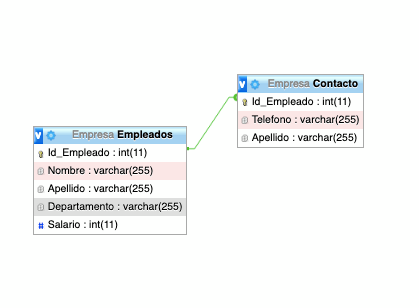
\includegraphics[width=226.9127pt,height=130.1pt]{latexImage_029a2dd6600756c21d6e5edbb0b6bddc.png}}
\put(295.3906,-180.8509){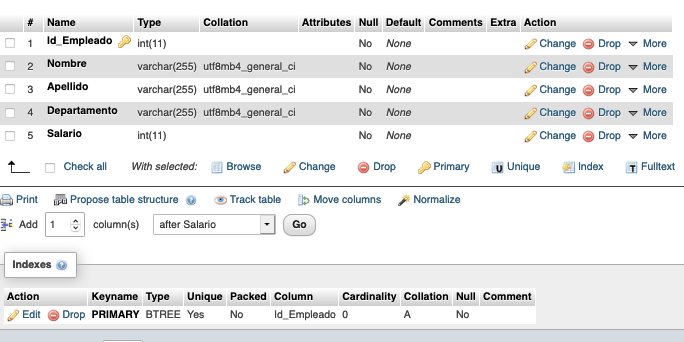
\includegraphics[width=271.9371pt,height=142.35pt]{latexImage_5aa95ed820e4bd9edcee359f6e1a8968.png}}
\put(295.3906,-569.5557){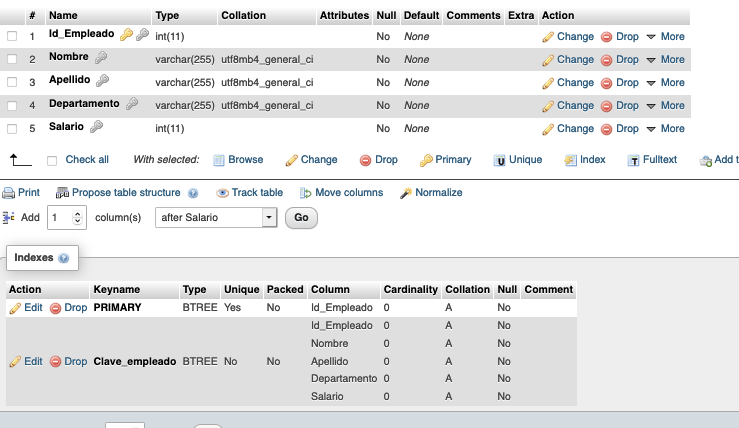
\includegraphics[width=252.4317pt,height=146.2pt]{latexImage_cb9e050616eda6cdf23c12de1cc08168.png}}
\end{picture}
\newpage
\begin{tikzpicture}[overlay]\path(0pt,0pt);\end{tikzpicture}
\begin{picture}(-5,0)(2.5,0)
\put(269.3906,-233.6608){\fontsize{10.08}{1}\usefont{T1}{cmr}{m}{n}\selectfont\color{color_29791} }
\put(33.47067,-242.7808){\fontsize{10.08}{1}\usefont{T1}{cmr}{m}{n}\selectfont\color{color_29791}El resultado de esta en la fila Id\_Empleado = 11 ya no }
\put(33.47067,-254.3008){\fontsize{10.08}{1}\usefont{T1}{cmr}{m}{n}\selectfont\color{color_29791}existirá.  }
\put(33.47067,-265.8208){\fontsize{10.08}{1}\usefont{T1}{cmr}{m}{n}\selectfont\color{color_29791} }
\put(33.47067,-277.3408){\fontsize{10.08}{1}\usefont{T1}{cmr}{m}{n}\selectfont\color{color_29791} }
\put(33.47067,-289.1008){\fontsize{10.08}{1}\usefont{T1}{cmr}{m}{n}\selectfont\color{color_29791} }
\put(33.47067,-300.6208){\fontsize{10.08}{1}\usefont{T1}{cmr}{m}{n}\selectfont\color{color_29791} }
\put(33.47067,-312.1408){\fontsize{10.08}{1}\usefont{T1}{cmr}{m}{n}\selectfont\color{color_29791}Si se desea eliminar todos los registros, la sintaxis seria la }
\put(33.47067,-323.6608){\fontsize{10.08}{1}\usefont{T1}{cmr}{m}{n}\selectfont\color{color_29791}siguiente: }
\put(33.47067,-335.1808){\fontsize{10.08}{1}\usefont{T1}{cmr}{m}{n}\selectfont\color{color_29791}DELETE FROM Empleados }
\put(33.47067,-346.7008){\fontsize{10.08}{1}\usefont{T1}{cmr}{m}{n}\selectfont\color{color_29791} }
\put(33.47067,-358.2208){\fontsize{10.08}{1}\usefont{T1}{cmr}{m}{n}\selectfont\color{color_29791}Para Borrar Una Tabla Completa De Una BB.BB. Se }
\put(33.47067,-369.7408){\fontsize{10.08}{1}\usefont{T1}{cmr}{m}{n}\selectfont\color{color_29791}Utiliza El Comando Drop Table: }
\put(33.47067,-381.2608){\fontsize{10.08}{1}\usefont{T1}{cmr}{m}{n}\selectfont\color{color_29791}DROP TABLE Empleados }
\put(33.47067,-393.0208){\fontsize{10.08}{1}\usefont{T1}{cmr}{m}{n}\selectfont\color{color_29791} }
\put(33.47067,-404.5408){\fontsize{10.08}{1}\usefont{T1}{cmr}{m}{n}\selectfont\color{color_29791}Y Para Borrar Un Índice: }
\put(33.47067,-416.0608){\fontsize{10.08}{1}\usefont{T1}{cmr}{m}{n}\selectfont\color{color_29791}DROP INDEX Clave\_Empleado; }
\put(33.47067,-427.5808){\fontsize{10.08}{1}\usefont{T1}{cmr}{m}{n}\selectfont\color{color_29791} }
\put(33.47067,-439.1008){\fontsize{10.08}{1}\usefont{T1}{cmr}{m}{n}\selectfont\color{color_29791}Para Afrontar Actualizaciones, En SQL Existe El Comando }
\put(33.47067,-450.6208){\fontsize{10.08}{1}\usefont{T1}{cmr}{m}{n}\selectfont\color{color_29791}‘update’: }
\put(33.47067,-462.1408){\fontsize{10.08}{1}\usefont{T1}{cmr}{m}{n}\selectfont\color{color_30045}UPDATE Empleados SET Nombre = "Donald", }
\end{picture}
\begin{tikzpicture}[overlay]
\path(0pt,0pt);
\filldraw[color_30045][nonzero rule]
(33.4706pt, -462.8608pt) -- (72.8306pt, -462.8608pt)
 -- (72.8306pt, -462.8608pt)
 -- (72.8306pt, -463.3408pt)
 -- (72.8306pt, -463.3408pt)
 -- (33.4706pt, -463.3408pt) -- cycle
;
\filldraw[color_30045][nonzero rule]
(122.2706pt, -462.8608pt) -- (140.0306pt, -462.8608pt)
 -- (140.0306pt, -462.8608pt)
 -- (140.0306pt, -463.3408pt)
 -- (140.0306pt, -463.3408pt)
 -- (122.2706pt, -463.3408pt) -- cycle
;
\end{tikzpicture}
\begin{picture}(-5,0)(2.5,0)
\put(33.47067,-473.6608){\fontsize{10.08}{1}\usefont{T1}{cmr}{m}{n}\selectfont\color{color_29791}Departamento = "IT" WHERE Id\_Empleado = "9" ; }
\put(33.47067,-485.4208){\fontsize{10.08}{1}\usefont{T1}{cmr}{m}{n}\selectfont\color{color_29791} }
\put(33.47067,-496.9408){\fontsize{10.08}{1}\usefont{T1}{cmr}{m}{n}\selectfont\color{color_29791} }
\put(269.3906,-531.2608){\fontsize{10.08}{1}\usefont{T1}{cmr}{m}{n}\selectfont\color{color_29791} }
\put(33.47067,-540.3808){\fontsize{10.08}{1}\usefont{T1}{cmr}{m}{n}\selectfont\color{color_29791} }
\put(33.47067,-551.9008){\fontsize{10.08}{1}\usefont{T1}{cmr}{m}{n}\selectfont\color{color_29791} }
\put(33.47067,-563.6608){\fontsize{10.08}{1}\usefont{T1}{cmr}{m}{n}\selectfont\color{color_29791} }
\put(33.47067,-575.1808){\fontsize{10.08}{1}\usefont{T1}{cmr}{m}{n}\selectfont\color{color_29791} }
\put(33.47067,-586.7008){\fontsize{10.08}{1}\usefont{T1}{cmr}{m}{n}\selectfont\color{color_29791} }
\put(33.47067,-598.2208){\fontsize{10.08}{1}\usefont{T1}{cmr}{m}{n}\selectfont\color{color_29791} }
\put(33.47067,-609.7408){\fontsize{10.08}{1}\usefont{T1}{cmr}{m}{n}\selectfont\color{color_29791} }
\put(33.47067,-621.2608){\fontsize{10.08}{1}\usefont{T1}{cmr}{m}{n}\selectfont\color{color_29791} }
\put(33.47067,-632.7808){\fontsize{10.08}{1}\usefont{T1}{cmr}{m}{n}\selectfont\color{color_29791} }
\put(33.47067,-644.3008){\fontsize{10.08}{1}\usefont{T1}{cmr}{m}{n}\selectfont\color{color_29791} }
\put(33.47067,-655.8208){\fontsize{10.08}{1}\usefont{T1}{cmr}{m}{n}\selectfont\color{color_29791}Consultas De Acción: Son comandos a ejecutar sobre las }
\put(33.47067,-667.5808){\fontsize{10.08}{1}\usefont{T1}{cmr}{m}{n}\selectfont\color{color_29791}tablas Tablas como: Modificación, borrado, inserción de }
\put(33.47067,-679.1008){\fontsize{10.08}{1}\usefont{T1}{cmr}{m}{n}\selectfont\color{color_29791}registro, y otros. }
\put(51.47067,-691.1008){\fontsize{10.08}{1}\usefont{T1}{cmr}{m}{n}\selectfont\color{color_29791}- INSERCIÓN, consiste en añadir nuevos registros }
\put(69.47067,-702.6208){\fontsize{10.08}{1}\usefont{T1}{cmr}{m}{n}\selectfont\color{color_29791}en las tablas, ej.: }
\put(33.47067,-714.1408){\fontsize{10.08}{1}\usefont{T1}{cmr}{m}{n}\selectfont\color{color_30045}INSERT INTO \`Empleados\` (\`Id\_Empleado\`, \`Nombre\`, }
\end{picture}
\begin{tikzpicture}[overlay]
\path(0pt,0pt);
\filldraw[color_30045][nonzero rule]
(33.4706pt, -714.8608pt) -- (68.5106pt, -714.8608pt)
 -- (68.5106pt, -714.8608pt)
 -- (68.5106pt, -715.3408pt)
 -- (68.5106pt, -715.3408pt)
 -- (33.4706pt, -715.3408pt) -- cycle
;
\end{tikzpicture}
\begin{picture}(-5,0)(2.5,0)
\put(33.47067,-725.6608){\fontsize{10.08}{1}\usefont{T1}{cmr}{m}{n}\selectfont\color{color_29791}\`Apellido\`, \`Departamento\`, \`Salario\`) VALUES (NULL, }
\end{picture}
\begin{tikzpicture}[overlay]
\path(0pt,0pt);
\filldraw[color_30045][nonzero rule]
(189.2306pt, -726.3808pt) -- (228.5906pt, -726.3808pt)
 -- (228.5906pt, -726.3808pt)
 -- (228.5906pt, -726.8608pt)
 -- (228.5906pt, -726.8608pt)
 -- (189.2306pt, -726.8608pt) -- cycle
;
\end{tikzpicture}
\begin{picture}(-5,0)(2.5,0)
\put(33.47067,-737.1808){\fontsize{10.08}{1}\usefont{T1}{cmr}{m}{n}\selectfont\color{color_29791}'Luis', 'Saldiver', 'Contabilidad', '340000'), (NULL, 'Laura', }
\put(33.47067,-748.7008){\fontsize{10.08}{1}\usefont{T1}{cmr}{m}{n}\selectfont\color{color_29791}'Perez', 'IT', '480000'), (NULL, 'Estela', 'Mardonez', }
\put(33.47067,-760.2208){\fontsize{10.08}{1}\usefont{T1}{cmr}{m}{n}\selectfont\color{color_29791}'Mercadeo', '360000'), (NULL, 'Maria', 'Lara', 'Ventas', }
\put(33.47067,-771.9808){\fontsize{10.08}{1}\usefont{T1}{cmr}{m}{n}\selectfont\color{color_29791}'980000'), (NULL, 'Jose', 'Gutierrez', 'Finanzas', '150000'), }
\put(33.47067,-783.5008){\fontsize{10.08}{1}\usefont{T1}{cmr}{m}{n}\selectfont\color{color_29791}(NULL, 'Pedro', 'Zerpa', 'Contabilidad', '400000'), (NULL, }
\put(33.47067,-795.0208){\fontsize{10.08}{1}\usefont{T1}{cmr}{m}{n}\selectfont\color{color_29791}'Esteban', 'Saldiver', 'IT', '289000'), (NULL, 'Luisa', 'Perez', }
\put(33.47067,-806.5408){\fontsize{10.08}{1}\usefont{T1}{cmr}{m}{n}\selectfont\color{color_29791}'Mercadeo', '545000'), (NULL, 'Jaime', 'Mardonez', 'Ventas', }
\put(294.5906,-46.70081){\fontsize{10.08}{1}\usefont{T1}{cmr}{m}{n}\selectfont\color{color_29791}'600000'), (NULL, 'Loreto', 'Lara', 'Finanzas', '388000'), }
\put(294.5906,-58.22083){\fontsize{10.08}{1}\usefont{T1}{cmr}{m}{n}\selectfont\color{color_29791}(NULL, 'Estefani', 'Gutierrez', 'Finanzas', '290000'), (NULL, }
\put(294.5906,-69.74084){\fontsize{10.08}{1}\usefont{T1}{cmr}{m}{n}\selectfont\color{color_29791}'Angel', 'Campos', 'IT', '780000'); }
\put(312.5906,-81.2608){\fontsize{10.08}{1}\usefont{T1}{cmr}{m}{n}\selectfont\color{color_29791} }
\put(312.5906,-92.78082){\fontsize{10.08}{1}\usefont{T1}{cmr}{m}{n}\selectfont\color{color_29791} }
\put(312.5906,-104.5408){\fontsize{10.08}{1}\usefont{T1}{cmr}{m}{n}\selectfont\color{color_29791} }
\put(550.4306,-319.3408){\fontsize{10.08}{1}\usefont{T1}{cmr}{m}{n}\selectfont\color{color_29791} }
\put(294.5906,-328.4608){\fontsize{10.08}{1}\usefont{T1}{cmr}{m}{n}\selectfont\color{color_29791} }
\put(294.5906,-339.9808){\fontsize{10.08}{1}\usefont{T1}{cmr}{m}{n}\selectfont\color{color_29791} }
\put(294.5906,-351.5008){\fontsize{10.08}{1}\usefont{T1}{cmr}{m}{n}\selectfont\color{color_29791} }
\put(294.5906,-363.0208){\fontsize{10.08}{1}\usefont{T1}{cmr}{m}{n}\selectfont\color{color_29791}Consultas De Selección Avanzadas }
\put(294.5906,-374.5408){\fontsize{10.08}{1}\usefont{T1}{cmr}{m}{n}\selectfont\color{color_29791}Esto Se Logra Mediante Cláusulas Como, Where, Group By, }
\put(294.5906,-386.0608){\fontsize{10.08}{1}\usefont{T1}{cmr}{m}{n}\selectfont\color{color_29791}Having Y Order By, Que Aumentan El Valor De Select. }
\put(294.5906,-397.5808){\fontsize{10.08}{1}\usefont{T1}{cmr}{m}{n}\selectfont\color{color_30045}SELECT Nombre FROM Empleados GROUP BY }
\end{picture}
\begin{tikzpicture}[overlay]
\path(0pt,0pt);
\filldraw[color_30045][nonzero rule]
(294.5906pt, -398.3008pt) -- (331.3106pt, -398.3008pt)
 -- (331.3106pt, -398.3008pt)
 -- (331.3106pt, -398.7808pt)
 -- (331.3106pt, -398.7808pt)
 -- (294.5906pt, -398.7808pt) -- cycle
;
\end{tikzpicture}
\begin{picture}(-5,0)(2.5,0)
\put(294.5906,-409.3408){\fontsize{10.08}{1}\usefont{T1}{cmr}{m}{n}\selectfont\color{color_29791}Id\_Empleado }
\put(294.5906,-420.8608){\fontsize{10.08}{1}\usefont{T1}{cmr}{m}{n}\selectfont\color{color_29791} }
\put(537.5707,-716.3008){\fontsize{10.08}{1}\usefont{T1}{cmr}{m}{n}\selectfont\color{color_29791} }
\put(294.5906,-725.4208){\fontsize{10.08}{1}\usefont{T1}{cmr}{m}{n}\selectfont\color{color_29791} }
\put(294.5906,-736.9408){\fontsize{10.08}{1}\usefont{T1}{cmr}{m}{n}\selectfont\color{color_29791} }
\put(294.5906,-748.4608){\fontsize{10.08}{1}\usefont{T1}{cmr}{m}{n}\selectfont\color{color_29791} }
\put(294.5906,-759.9808){\fontsize{10.08}{1}\usefont{T1}{cmr}{m}{n}\selectfont\color{color_29791}Clausula, HAVING (Requiere Registros Previamente }
\put(294.5906,-771.5008){\fontsize{10.08}{1}\usefont{T1}{cmr}{m}{n}\selectfont\color{color_29791}Agrupados): }
\put(294.5906,-783.0208){\fontsize{10.08}{1}\usefont{T1}{cmr}{m}{n}\selectfont\color{color_30045}SELECT Id\_Empleado,SUM(Salario) FROM Empleados }
\end{picture}
\begin{tikzpicture}[overlay]
\path(0pt,0pt);
\filldraw[color_30045][nonzero rule]
(294.5906pt, -783.7408pt) -- (331.3106pt, -783.7408pt)
 -- (331.3106pt, -783.7408pt)
 -- (331.3106pt, -784.2208pt)
 -- (331.3106pt, -784.2208pt)
 -- (294.5906pt, -784.2208pt) -- cycle
;
\filldraw[color_30045][nonzero rule]
(390.1106pt, -783.7408pt) -- (411.7106pt, -783.7408pt)
 -- (411.7106pt, -783.7408pt)
 -- (411.7106pt, -784.2208pt)
 -- (411.7106pt, -784.2208pt)
 -- (390.1106pt, -784.2208pt) -- cycle
;
\end{tikzpicture}
\begin{picture}(-5,0)(2.5,0)
\put(294.5906,-794.5408){\fontsize{10.08}{1}\usefont{T1}{cmr}{m}{n}\selectfont\color{color_29791}GROUP BY Id\_Empleado HAVING SUM(Salario)>300000  }
\end{picture}
\begin{tikzpicture}[overlay]
\path(0pt,0pt);
\filldraw[color_30045][nonzero rule]
(445.7906pt, -795.2608pt) -- (467.3906pt, -795.2608pt)
 -- (467.3906pt, -795.2608pt)
 -- (467.3906pt, -795.7408pt)
 -- (467.3906pt, -795.7408pt)
 -- (445.7906pt, -795.7408pt) -- cycle
;
\end{tikzpicture}
\begin{picture}(-5,0)(2.5,0)
\put(294.5906,-806.0608){\fontsize{10.08}{1}\usefont{T1}{cmr}{m}{n}\selectfont\color{color_29791} }
\put(34.3906,-234.6009){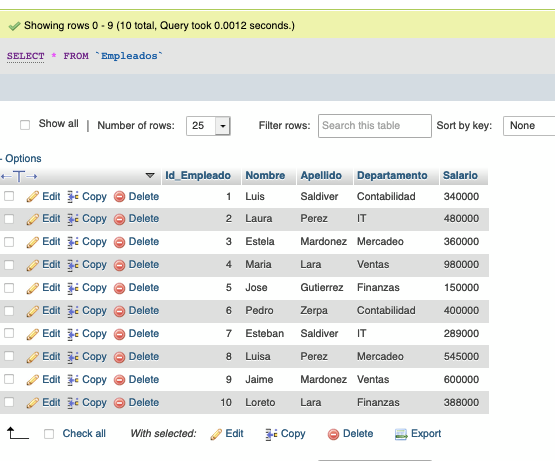
\includegraphics[width=236.0767pt,height=196.1pt]{latexImage_3f6b737c362b953150216db7fafb0711.png}}
\put(34.3906,-532.2515){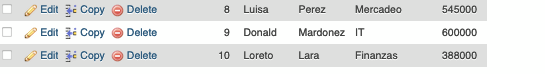
\includegraphics[width=236.0254pt,height=32.05pt]{latexImage_2e50c2adc60c2db8056b971983da4f94.png}}
\put(295.3906,-320.1879){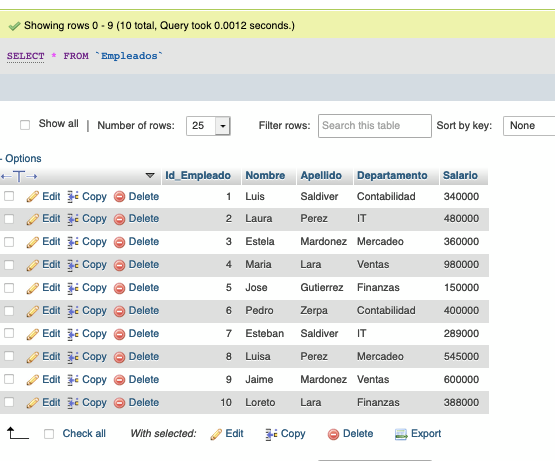
\includegraphics[width=255.6995pt,height=212.4pt]{latexImage_3f6b737c362b953150216db7fafb0711.png}}
\put(297.3906,-716.9184){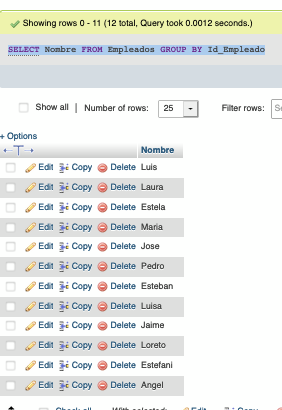
\includegraphics[width=240.55pt,height=292.8pt]{latexImage_dbae88d863c1f7c69e529187ee8d4389.png}}
\end{picture}
\newpage
\begin{tikzpicture}[overlay]\path(0pt,0pt);\end{tikzpicture}
\begin{picture}(-5,0)(2.5,0)
\put(270.5908,-177.7408){\fontsize{10.08}{1}\usefont{T1}{cmr}{m}{n}\selectfont\color{color_29791} }
\put(33.47067,-186.8608){\fontsize{10.08}{1}\usefont{T1}{cmr}{m}{n}\selectfont\color{color_29791} }
\put(33.47067,-198.3808){\fontsize{10.08}{1}\usefont{T1}{cmr}{m}{n}\selectfont\color{color_29791} }
\put(33.47067,-210.1408){\fontsize{10.08}{1}\usefont{T1}{cmr}{m}{n}\selectfont\color{color_29791} }
\put(33.47067,-221.6608){\fontsize{10.08}{1}\usefont{T1}{cmr}{m}{n}\selectfont\color{color_29791} }
\put(33.47067,-233.1808){\fontsize{10.08}{1}\usefont{T1}{cmr}{m}{n}\selectfont\color{color_29791} }
\put(33.47067,-244.7008){\fontsize{10.08}{1}\usefont{T1}{cmr}{m}{n}\selectfont\color{color_29791} }
\put(33.47067,-256.2208){\fontsize{10.08}{1}\usefont{T1}{cmr}{m}{n}\selectfont\color{color_29791} }
\put(33.47067,-267.7408){\fontsize{10.08}{1}\usefont{T1}{cmr}{m}{n}\selectfont\color{color_29791} }
\put(33.47067,-279.2608){\fontsize{10.08}{1}\usefont{T1}{cmr}{m}{n}\selectfont\color{color_29791} }
\put(33.47067,-290.7808){\fontsize{10.08}{1}\usefont{T1}{cmr}{m}{n}\selectfont\color{color_29791} }
\put(33.47067,-302.5408){\fontsize{10.08}{1}\usefont{T1}{cmr}{m}{n}\selectfont\color{color_29791}Intersecciones: }
\put(33.47067,-314.0608){\fontsize{10.08}{1}\usefont{T1}{cmr}{m}{n}\selectfont\color{color_29791}Tomando en cuenta que se creó la base de datos ‘Contacto’, }
\put(33.47067,-325.5808){\fontsize{10.08}{1}\usefont{T1}{cmr}{m}{n}\selectfont\color{color_29791}la sintaxis es: }
\put(33.47067,-337.1008){\fontsize{10.08}{1}\usefont{T1}{cmr}{m}{n}\selectfont\color{color_30045}CREATE TABLE \`Contacto\`.\`3\` ( \`Id\_Empleado\` INT(11) }
\end{picture}
\begin{tikzpicture}[overlay]
\path(0pt,0pt);
\filldraw[color_30045][nonzero rule]
(33.4706pt, -337.8208pt) -- (72.3506pt, -337.8208pt)
 -- (72.3506pt, -337.8208pt)
 -- (72.3506pt, -338.3008pt)
 -- (72.3506pt, -338.3008pt)
 -- (33.4706pt, -338.3008pt) -- cycle
;
\filldraw[color_30045][nonzero rule]
(74.7506pt, -337.8208pt) -- (107.1506pt, -337.8208pt)
 -- (107.1506pt, -337.8208pt)
 -- (107.1506pt, -338.3008pt)
 -- (107.1506pt, -338.3008pt)
 -- (74.7506pt, -338.3008pt) -- cycle
;
\filldraw[color_30045][nonzero rule]
(237.9506pt, -337.8208pt) -- (254.5106pt, -337.8208pt)
 -- (254.5106pt, -337.8208pt)
 -- (254.5106pt, -338.3008pt)
 -- (254.5106pt, -338.3008pt)
 -- (237.9506pt, -338.3008pt) -- cycle
;
\end{tikzpicture}
\begin{picture}(-5,0)(2.5,0)
\put(33.47067,-348.6208){\fontsize{10.08}{1}\usefont{T1}{cmr}{m}{n}\selectfont\color{color_29791}NULL AUTO\_INCREMENT , \`Telefono\` }
\put(33.47067,-360.1408){\fontsize{10.08}{1}\usefont{T1}{cmr}{m}{n}\selectfont\color{color_30045}VARCHAR(255) NOT NULL , \`Apellido\` }
\end{picture}
\begin{tikzpicture}[overlay]
\path(0pt,0pt);
\filldraw[color_30045][nonzero rule]
(33.4706pt, -360.8608pt) -- (82.4306pt, -360.8608pt)
 -- (82.4306pt, -360.8608pt)
 -- (82.4306pt, -361.3408pt)
 -- (82.4306pt, -361.3408pt)
 -- (33.4706pt, -361.3408pt) -- cycle
;
\filldraw[color_30045][nonzero rule]
(106.4306pt, -360.8608pt) -- (127.0706pt, -360.8608pt)
 -- (127.0706pt, -360.8608pt)
 -- (127.0706pt, -361.3408pt)
 -- (127.0706pt, -361.3408pt)
 -- (106.4306pt, -361.3408pt) -- cycle
;
\end{tikzpicture}
\begin{picture}(-5,0)(2.5,0)
\put(33.47067,-371.6608){\fontsize{10.08}{1}\usefont{T1}{cmr}{m}{n}\selectfont\color{color_30045}VARCHAR(255) NOT NULL , PRIMARY KEY }
\end{picture}
\begin{tikzpicture}[overlay]
\path(0pt,0pt);
\filldraw[color_30045][nonzero rule]
(33.4706pt, -372.3808pt) -- (82.4306pt, -372.3808pt)
 -- (82.4306pt, -372.3808pt)
 -- (82.4306pt, -372.8608pt)
 -- (82.4306pt, -372.8608pt)
 -- (33.4706pt, -372.8608pt) -- cycle
;
\filldraw[color_30045][nonzero rule]
(106.4306pt, -372.3808pt) -- (127.0706pt, -372.3808pt)
 -- (127.0706pt, -372.3808pt)
 -- (127.0706pt, -372.8608pt)
 -- (127.0706pt, -372.8608pt)
 -- (106.4306pt, -372.8608pt) -- cycle
;
\end{tikzpicture}
\begin{picture}(-5,0)(2.5,0)
\put(33.47067,-383.1808){\fontsize{10.08}{1}\usefont{T1}{cmr}{m}{n}\selectfont\color{color_29791}(\`Id\_Empleado\`)) ENGINE = InnoDB;  }
\put(33.47067,-394.7008){\fontsize{10.08}{1}\usefont{T1}{cmr}{m}{n}\selectfont\color{color_29791} }
\put(274.4306,-525.2608){\fontsize{10.08}{1}\usefont{T1}{cmr}{m}{n}\selectfont\color{color_29791} }
\put(33.47067,-534.3808){\fontsize{10.08}{1}\usefont{T1}{cmr}{m}{n}\selectfont\color{color_29791} }
\put(33.47067,-545.9008){\fontsize{10.08}{1}\usefont{T1}{cmr}{m}{n}\selectfont\color{color_29791} }
\put(33.47067,-557.4208){\fontsize{10.08}{1}\usefont{T1}{cmr}{m}{n}\selectfont\color{color_29791} }
\put(33.47067,-568.9408){\fontsize{10.08}{1}\usefont{T1}{cmr}{m}{n}\selectfont\color{color_29791} }
\put(33.47067,-580.4608){\fontsize{10.08}{1}\usefont{T1}{cmr}{m}{n}\selectfont\color{color_29791} }
\put(33.47067,-591.9808){\fontsize{10.08}{1}\usefont{T1}{cmr}{m}{n}\selectfont\color{color_29791} }
\put(33.47067,-603.7408){\fontsize{10.08}{1}\usefont{T1}{cmr}{m}{n}\selectfont\color{color_29791} }
\put(33.47067,-615.2608){\fontsize{10.08}{1}\usefont{T1}{cmr}{m}{n}\selectfont\color{color_29791} }
\put(33.47067,-626.7808){\fontsize{10.08}{1}\usefont{T1}{cmr}{m}{n}\selectfont\color{color_29791}Inserto datos: }
\put(33.47067,-638.3008){\fontsize{10.08}{1}\usefont{T1}{cmr}{m}{n}\selectfont\color{color_30045}INSERT INTO \`3\` (\`Id\_Empleado\`, \`Telefono\`, \`Apellido\`) }
\end{picture}
\begin{tikzpicture}[overlay]
\path(0pt,0pt);
\filldraw[color_30045][nonzero rule]
(33.4706pt, -639.0208pt) -- (68.5106pt, -639.0208pt)
 -- (68.5106pt, -639.0208pt)
 -- (68.5106pt, -639.5008pt)
 -- (68.5106pt, -639.5008pt)
 -- (33.4706pt, -639.5008pt) -- cycle
;
\end{tikzpicture}
\begin{picture}(-5,0)(2.5,0)
\put(33.47067,-649.8208){\fontsize{10.08}{1}\usefont{T1}{cmr}{m}{n}\selectfont\color{color_30045}VALUES (NULL, '955787689', 'Saldiver'), (NULL, }
\end{picture}
\begin{tikzpicture}[overlay]
\path(0pt,0pt);
\filldraw[color_30045][nonzero rule]
(33.4706pt, -650.5408pt) -- (72.8306pt, -650.5408pt)
 -- (72.8306pt, -650.5408pt)
 -- (72.8306pt, -651.0208pt)
 -- (72.8306pt, -651.0208pt)
 -- (33.4706pt, -651.0208pt) -- cycle
;
\end{tikzpicture}
\begin{picture}(-5,0)(2.5,0)
\put(33.47067,-661.3408){\fontsize{10.08}{1}\usefont{T1}{cmr}{m}{n}\selectfont\color{color_29791}'964356545', 'Perez'), (NULL, '987445323', 'Mardonez'), }
\put(33.47067,-672.8608){\fontsize{10.08}{1}\usefont{T1}{cmr}{m}{n}\selectfont\color{color_29791}(NULL, '934558879', 'Lara')  }
\put(33.47067,-684.3808){\fontsize{10.08}{1}\usefont{T1}{cmr}{m}{n}\selectfont\color{color_29791} }
\put(271.8657,-793.1008){\fontsize{10.08}{1}\usefont{T1}{cmr}{m}{n}\selectfont\color{color_29791} }
\put(33.47067,-802.2208){\fontsize{10.08}{1}\usefont{T1}{cmr}{m}{n}\selectfont\color{color_29791} ‘Union’ permite combinar los registros obtenidos mediante }
\put(33.47067,-813.7408){\fontsize{10.08}{1}\usefont{T1}{cmr}{m}{n}\selectfont\color{color_29791}la ejecución de dos o mas cláusulas, que deben contemplar }
\put(294.5906,-46.70081){\fontsize{10.08}{1}\usefont{T1}{cmr}{m}{n}\selectfont\color{color_29791}la misma cantidad de columnas.  }
\put(294.5906,-58.22083){\fontsize{10.08}{1}\usefont{T1}{cmr}{m}{n}\selectfont\color{color_30045}SELECT Id\_Empleado, Nombre FROM Empleados UNION }
\end{picture}
\begin{tikzpicture}[overlay]
\path(0pt,0pt);
\filldraw[color_30045][nonzero rule]
(294.5906pt, -58.9408pt) -- (331.3106pt, -58.9408pt)
 -- (331.3106pt, -58.9408pt)
 -- (331.3106pt, -59.42078pt)
 -- (331.3106pt, -59.42078pt)
 -- (294.5906pt, -59.42078pt) -- cycle
;
\end{tikzpicture}
\begin{picture}(-5,0)(2.5,0)
\put(294.5906,-69.74084){\fontsize{10.08}{1}\usefont{T1}{cmr}{m}{n}\selectfont\color{color_30045}SELECT Id\_Empleado, Telefono FROM Contacto; }
\end{picture}
\begin{tikzpicture}[overlay]
\path(0pt,0pt);
\filldraw[color_30045][nonzero rule]
(294.5906pt, -70.46082pt) -- (331.3106pt, -70.46082pt)
 -- (331.3106pt, -70.46082pt)
 -- (331.3106pt, -70.9408pt)
 -- (331.3106pt, -70.9408pt)
 -- (294.5906pt, -70.9408pt) -- cycle
;
\end{tikzpicture}
\begin{picture}(-5,0)(2.5,0)
\put(294.5906,-81.2608){\fontsize{10.08}{1}\usefont{T1}{cmr}{m}{n}\selectfont\color{color_29791} }
\put(520.9106,-214.7008){\fontsize{10.08}{1}\usefont{T1}{cmr}{m}{n}\selectfont\color{color_29791} }
\put(294.5906,-223.8208){\fontsize{10.08}{1}\usefont{T1}{cmr}{m}{n}\selectfont\color{color_29791} }
\put(294.5906,-235.3408){\fontsize{10.08}{1}\usefont{T1}{cmr}{m}{n}\selectfont\color{color_29791}SQL mantiene un conjunto de comandos que logran manejar }
\put(294.5906,-247.1008){\fontsize{10.08}{1}\usefont{T1}{cmr}{m}{n}\selectfont\color{color_29791}bases de datos de una forma fácil e intuitiva. La cláusula }
\put(294.5906,-258.6208){\fontsize{10.08}{1}\usefont{T1}{cmr}{m}{n}\selectfont\color{color_29791}SELECT siempre tiene una gran versatilidad, Permite la }
\put(294.5906,-270.1408){\fontsize{10.08}{1}\usefont{T1}{cmr}{m}{n}\selectfont\color{color_29791}realización de cualquier tipo de consulta sobre los datos.  }
\put(294.5906,-281.6608){\fontsize{10.08}{1}\usefont{T1}{cmr}{m}{n}\selectfont\color{color_29791}Estas características han hecho de SQL el lenguaje preferido }
\put(294.5906,-293.1808){\fontsize{10.08}{1}\usefont{T1}{cmr}{m}{n}\selectfont\color{color_29791}para el manejo y gestión de los sistemas de bases de datos, lo }
\put(294.5906,-304.7008){\fontsize{10.08}{1}\usefont{T1}{cmr}{m}{n}\selectfont\color{color_29791}cual ha generado que se desarrollen diferentes versiones para }
\put(294.5906,-316.2208){\fontsize{10.08}{1}\usefont{T1}{cmr}{m}{n}\selectfont\color{color_29791}ser usadas en entornos más específicos. }
\put(294.5906,-327.7408){\fontsize{10.08}{1}\usefont{T1}{cmr}{m}{n}\selectfont\color{color_29791} }
\put(294.5906,-339.2608){\fontsize{10.08}{1}\usefont{T1}{cmr}{m}{n}\selectfont\color{color_29791} }
\put(294.5906,-351.0208){\fontsize{10.08}{1}\usefont{T1}{cmr}{m}{n}\selectfont\color{color_29791} }
\put(294.5906,-362.5408){\fontsize{10.08}{1}\usefont{T1}{cmr}{m}{n}\selectfont\color{color_29791}Originalmente MySQL era un software propietario, 5 }
\put(294.5906,-374.0608){\fontsize{10.08}{1}\usefont{T1}{cmr}{m}{n}\selectfont\color{color_29791}años después de 1995 se volvió OpenSource con soporte }
\put(294.5906,-385.5808){\fontsize{10.08}{1}\usefont{T1}{cmr}{m}{n}\selectfont\color{color_29791}para Linux-Unix.  }
\put(294.5906,-397.1008){\fontsize{10.08}{1}\usefont{T1}{cmr}{m}{n}\selectfont\color{color_29791}MySQL no estuvo orientado a una gran escala, su uso era }
\put(294.5906,-408.6208){\fontsize{10.08}{1}\usefont{T1}{cmr}{m}{n}\selectfont\color{color_29791}mas bien practico. Fué tan bien escrito, que se convirtió en }
\put(294.5906,-420.1408){\fontsize{10.08}{1}\usefont{T1}{cmr}{m}{n}\selectfont\color{color_29791}un DBMS preferido. }
\put(294.5906,-431.6608){\fontsize{10.08}{1}\usefont{T1}{cmr}{m}{n}\selectfont\color{color_29791}Su instalación difiere un poco dependiendo de ciertos }
\put(294.5906,-443.4208){\fontsize{10.08}{1}\usefont{T1}{cmr}{m}{n}\selectfont\color{color_29791}aspectos, como:  }
\put(312.5906,-455.4208){\fontsize{10.08}{1}\usefont{T1}{cmr}{m}{n}\selectfont\color{color_29791}- Establecer compatibilidad para MySQL, se requiere }
\put(330.5906,-466.9408){\fontsize{10.08}{1}\usefont{T1}{cmr}{m}{n}\selectfont\color{color_29791}verificar si soporta y esta respaldado por la empresa }
\put(330.5906,-478.4608){\fontsize{10.08}{1}\usefont{T1}{cmr}{m}{n}\selectfont\color{color_29791}Oracle Corp. }
\put(312.5906,-490.4608){\fontsize{10.08}{1}\usefont{T1}{cmr}{m}{n}\selectfont\color{color_29791}- Decidir cual distribución instalar, binario, o código }
\put(330.5906,-501.9808){\fontsize{10.08}{1}\usefont{T1}{cmr}{m}{n}\selectfont\color{color_29791}abierto (Permite acceso para desarrollo), verificar }
\put(330.5906,-513.5009){\fontsize{10.08}{1}\usefont{T1}{cmr}{m}{n}\selectfont\color{color_29791}descarga bajo Oracle Corp., Verificar bajo que O.S. }
\put(330.5906,-525.0208){\fontsize{10.08}{1}\usefont{T1}{cmr}{m}{n}\selectfont\color{color_29791}se instalará.  }
\put(312.5906,-537.0208){\fontsize{10.08}{1}\usefont{T1}{cmr}{m}{n}\selectfont\color{color_29791}- MySQL Community Server, descargable de manera }
\put(330.5906,-548.5408){\fontsize{10.08}{1}\usefont{T1}{cmr}{m}{n}\selectfont\color{color_29791}libre, para pequeños o medianos usuarios, soportada }
\put(330.5906,-560.3008){\fontsize{10.08}{1}\usefont{T1}{cmr}{m}{n}\selectfont\color{color_29791}bajo licencia GPL, así se tiene acceso a esta, como }
\put(330.5906,-571.8208){\fontsize{10.08}{1}\usefont{T1}{cmr}{m}{n}\selectfont\color{color_29791}código abierto, soportada para colaboradores y }
\put(330.5906,-583.3408){\fontsize{10.08}{1}\usefont{T1}{cmr}{m}{n}\selectfont\color{color_29791}Developers. }
\put(299.9407,-594.8608){\fontsize{10.08}{1}\usefont{T1}{cmr}{m}{n}\selectfont\color{color_29791} }
\put(294.5906,-606.3808){\fontsize{10.08}{1}\usefont{T1}{cmr}{m}{n}\selectfont\color{color_29791}Bajo la licencia GPL, existen limitaciones comparado a }
\put(294.5906,-617.9008){\fontsize{10.08}{1}\usefont{T1}{cmr}{m}{n}\selectfont\color{color_29791}Enterprise Edition que tiene funciones adicionales para el }
\put(294.5906,-629.4208){\fontsize{10.08}{1}\usefont{T1}{cmr}{m}{n}\selectfont\color{color_29791}ámbito empresarial. }
\put(294.5906,-640.9408){\fontsize{10.08}{1}\usefont{T1}{cmr}{m}{n}\selectfont\color{color_29791} }
\put(294.5906,-652.4608){\fontsize{10.08}{1}\usefont{T1}{cmr}{m}{n}\selectfont\color{color_29791}Se puede crear una tabla con un respectivo ID, por eje.: }
\put(294.5906,-664.2208){\fontsize{10.08}{1}\usefont{T1}{cmr}{m}{n}\selectfont\color{color_29791}CREATE TABLE Empleados (Nombre varchar(50), }
\put(294.5906,-675.7408){\fontsize{10.08}{1}\usefont{T1}{cmr}{m}{n}\selectfont\color{color_29791}Apellido varchar(50), ID int AUTOINCREMENT }
\put(294.5906,-687.2608){\fontsize{10.08}{1}\usefont{T1}{cmr}{m}{n}\selectfont\color{color_29791}PRIMARY KEY (ID) ); }
\put(294.5906,-698.7808){\fontsize{10.08}{1}\usefont{T1}{cmr}{m}{n}\selectfont\color{color_29791} }
\put(294.5906,-710.3008){\fontsize{10.08}{1}\usefont{T1}{cmr}{m}{n}\selectfont\color{color_29791}Para ingresar 10 registros en la tabla anterior considerando }
\put(294.5906,-721.8208){\fontsize{10.08}{1}\usefont{T1}{cmr}{m}{n}\selectfont\color{color_29791}que en la columna Apellido }
\put(294.5906,-733.3408){\fontsize{10.08}{1}\usefont{T1}{cmr}{m}{n}\selectfont\color{color_29791}cinco de ellos deben comenzar con la letra D.: }
\put(294.5906,-744.8608){\fontsize{10.08}{1}\usefont{T1}{cmr}{m}{n}\selectfont\color{color_29791} }
\put(294.5906,-756.6208){\fontsize{10.08}{1}\usefont{T1}{cmr}{m}{n}\selectfont\color{color_29791}INSERT INTO Empleados (Nombre, Apellido, ID) }
\put(294.5906,-768.1408){\fontsize{10.08}{1}\usefont{T1}{cmr}{m}{n}\selectfont\color{color_29791}VALUES (‘Dohn, ‘Lemon’, ‘’), (‘Daul’, ‘Martney’,’’), }
\put(294.5906,-779.6608){\fontsize{10.08}{1}\usefont{T1}{cmr}{m}{n}\selectfont\color{color_29791}(‘Detephen’, ‘Ding’,’’), (‘Daily’, ‘Moon’,’’), (‘Dinitry’, }
\put(294.5906,-791.1808){\fontsize{10.08}{1}\usefont{T1}{cmr}{m}{n}\selectfont\color{color_29791}‘Larry’,’’), (‘Stephen’, ‘King’,’’), (‘Larry’, ‘Olson’,’’), }
\put(294.5906,-802.7008){\fontsize{10.08}{1}\usefont{T1}{cmr}{m}{n}\selectfont\color{color_29791}(‘Peter’, ‘Woom’,’’), (‘Tonny’, ‘Waka’,’’), (‘David’, }
\put(294.5906,-814.2208){\fontsize{10.08}{1}\usefont{T1}{cmr}{m}{n}\selectfont\color{color_29791}‘B}
\put(34.3906,-178.7408){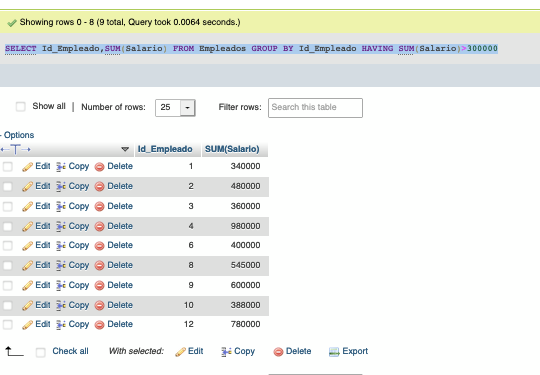
\includegraphics[width=237.25pt,height=140.24pt]{latexImage_09e5474c8b7ac09b7bc7703bae9b62bb.png}}
\put(34.3906,-525.76){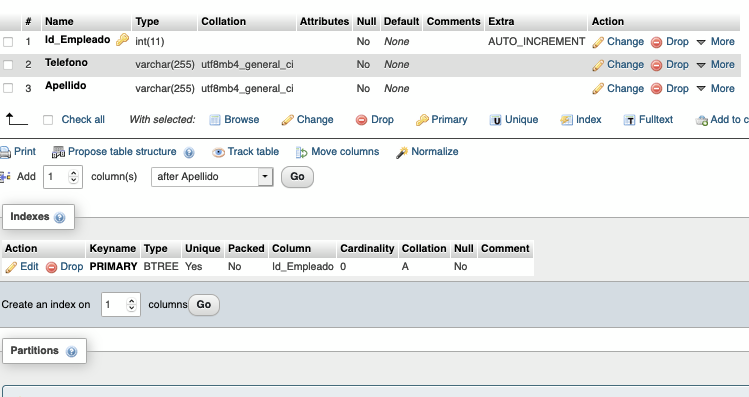
\includegraphics[width=240.745pt,height=127.6pt]{latexImage_c8abde8d9a9b3e6dd50b624087cada04.png}}
\put(37.31564,-793.9799){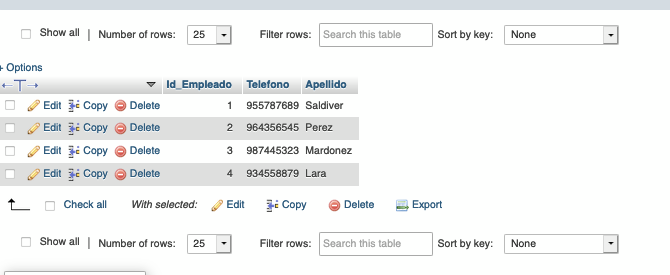
\includegraphics[width=235.4641pt,height=106.15pt]{latexImage_f43fcf35e77d94bb17669589d1e61f00.png}}
\put(295.3906,-215.3423){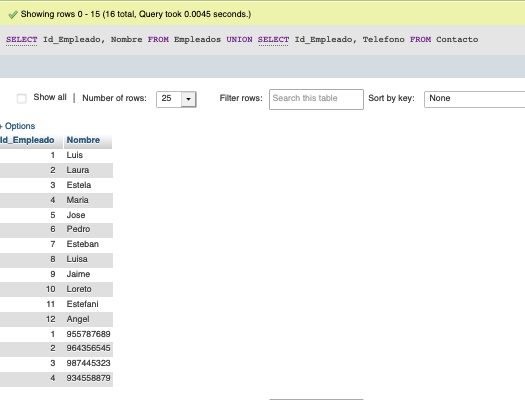
\includegraphics[width=226.3294pt,height=130.65pt]{latexImage_408ff130a82c4122fdc9c8aefbc6050c.png}}
\end{picture}
\newpage
\begin{tikzpicture}[overlay]\path(0pt,0pt);\end{tikzpicture}
\begin{picture}(-5,0)(2.5,0)
\put(33.47067,-46.70081){\fontsize{10.08}{1}\usefont{T1}{cmr}{m}{n}\selectfont\color{color_29791}Apellido like = “D\%”);  }
\put(33.47067,-58.22083){\fontsize{10.08}{1}\usefont{T1}{cmr}{m}{n}\selectfont\color{color_29791} }
\put(33.47067,-69.74084){\fontsize{10.08}{1}\usefont{T1}{cmr}{m}{n}\selectfont\color{color_29791}MySQL dispone de un optimizador de consultas y este }
\put(33.47067,-81.2608){\fontsize{10.08}{1}\usefont{T1}{cmr}{m}{n}\selectfont\color{color_29791}utiliza distribución de claves almacenadas y otros factores }
\put(33.47067,-92.78082){\fontsize{10.08}{1}\usefont{T1}{cmr}{m}{n}\selectfont\color{color_29791}para decidir el orden en que se deben unir las tablas y que }
\put(33.47067,-104.5408){\fontsize{10.08}{1}\usefont{T1}{cmr}{m}{n}\selectfont\color{color_29791}índice se debe usar para una tabla especifica.  }
\put(33.47067,-116.0608){\fontsize{10.08}{1}\usefont{T1}{cmr}{m}{n}\selectfont\color{color_29791}Las estructuras de datos almacenan información entre }
\put(33.47067,-127.5808){\fontsize{10.08}{1}\usefont{T1}{cmr}{m}{n}\selectfont\color{color_29791}objetos y relaciones entre ellas. Para ello utiliza el modelo }
\put(33.47067,-139.1008){\fontsize{10.08}{1}\usefont{T1}{cmr}{m}{n}\selectfont\color{color_29791}de entidad relación (ER). }
\put(33.47067,-150.6208){\fontsize{10.08}{1}\usefont{T1}{cmr}{m}{n}\selectfont\color{color_29791}Un modelo -ER- se construye de manera grafica mediante }
\put(33.47067,-162.1408){\fontsize{10.08}{1}\usefont{T1}{cmr}{m}{n}\selectfont\color{color_29791}símbolos como: }
\put(51.47067,-174.1408){\fontsize{10.08}{1}\usefont{T1}{cmr}{m}{n}\selectfont\color{color_29791}- Rectángulos. }
\put(51.47067,-186.1408){\fontsize{10.08}{1}\usefont{T1}{cmr}{m}{n}\selectfont\color{color_29791}- Líneas. }
\put(38.82078,-197.6608){\fontsize{10.08}{1}\usefont{T1}{cmr}{m}{n}\selectfont\color{color_29791} }
\put(33.47067,-209.4208){\fontsize{10.08}{1}\usefont{T1}{cmr}{m}{n}\selectfont\color{color_29791}Estas representan entidades en: }
\put(51.47067,-221.4208){\fontsize{10.08}{1}\usefont{T1}{cmr}{m}{n}\selectfont\color{color_29791}- Un proceso. }
\put(51.47067,-233.4208){\fontsize{10.08}{1}\usefont{T1}{cmr}{m}{n}\selectfont\color{color_29791}- Bajo características. }
\put(51.47067,-245.4208){\fontsize{10.08}{1}\usefont{T1}{cmr}{m}{n}\selectfont\color{color_29791}- Relaciones existentes. }
\put(33.47067,-256.9408){\fontsize{10.08}{1}\usefont{T1}{cmr}{m}{n}\selectfont\color{color_29791} }
\put(33.47067,-268.4608){\fontsize{10.08}{1}\usefont{T1}{cmr}{m}{n}\selectfont\color{color_29791} }
\put(33.47067,-279.9808){\fontsize{10.08}{1}\usefont{T1}{cmr}{m}{n}\selectfont\color{color_29791} }
\put(33.47067,-291.5008){\fontsize{10.08}{1}\usefont{T1}{cmr}{m}{n}\selectfont\color{color_29791}Las relaciones tienen elementos, como, objetos, atributos, }
\put(33.47067,-303.0208){\fontsize{10.08}{1}\usefont{T1}{cmr}{m}{n}\selectfont\color{color_29791}relaciones, tablas. }
\put(33.47067,-314.7808){\fontsize{10.08}{1}\usefont{T1}{cmr}{m}{n}\selectfont\color{color_29791} }
\put(33.47067,-326.3008){\fontsize{10.08}{1}\usefont{T1}{cmr}{m}{n}\selectfont\color{color_29791}Tablas: }
\put(33.47067,-337.8208){\fontsize{10.08}{1}\usefont{T1}{cmr}{m}{n}\selectfont\color{color_29791}Las tablas son estructuras donde se almacenan los datos, sin }
\put(33.47067,-349.3408){\fontsize{10.08}{1}\usefont{T1}{cmr}{m}{n}\selectfont\color{color_29791}estas, seria imposible el concepto de datos relacionales. }
\put(33.47067,-360.8608){\fontsize{10.08}{1}\usefont{T1}{cmr}{m}{n}\selectfont\color{color_29791}Para esto se deben considerar aspectos como: }
\put(51.47067,-372.8608){\fontsize{10.08}{1}\usefont{T1}{cmr}{m}{n}\selectfont\color{color_29791}- Cantidad. }
\put(51.47067,-384.8608){\fontsize{10.08}{1}\usefont{T1}{cmr}{m}{n}\selectfont\color{color_29791}- Numero de columnas. }
\put(51.47067,-396.8608){\fontsize{10.08}{1}\usefont{T1}{cmr}{m}{n}\selectfont\color{color_29791}- Tipo de dato. }
\put(38.82078,-408.3808){\fontsize{10.08}{1}\usefont{T1}{cmr}{m}{n}\selectfont\color{color_29791} }
\put(33.47067,-419.9008){\fontsize{10.08}{1}\usefont{T1}{cmr}{m}{n}\selectfont\color{color_29791}Para crear una tabla llamada Contacto\_Empleados, la que }
\put(33.47067,-431.6608){\fontsize{10.08}{1}\usefont{T1}{cmr}{m}{n}\selectfont\color{color_29791}debe contener las columnas }
\put(33.47067,-443.1808){\fontsize{10.08}{1}\usefont{T1}{cmr}{m}{n}\selectfont\color{color_29791}Identificación del empleado, número telefónico y correo }
\put(33.47067,-454.7008){\fontsize{10.08}{1}\usefont{T1}{cmr}{m}{n}\selectfont\color{color_29791}electrónico, su instrucción es la Sgte.: }
\put(33.47067,-466.2208){\fontsize{10.08}{1}\usefont{T1}{cmr}{m}{n}\selectfont\color{color_29791}CREATE TABLE IF NOT EXISTS Contacto\_Empleados }
\put(33.47067,-477.7408){\fontsize{10.08}{1}\usefont{T1}{cmr}{m}{n}\selectfont\color{color_29791}(identificación int AUTOINCREMENT }
\put(33.47067,-489.2608){\fontsize{10.08}{1}\usefont{T1}{cmr}{m}{n}\selectfont\color{color_29791}PRIMARY KEY (Id\_Empleado), Numero\_Tel varchar(50), }
\put(33.47067,-500.7808){\fontsize{10.08}{1}\usefont{T1}{cmr}{m}{n}\selectfont\color{color_29791}Email varchar(250) }
\put(33.47067,-512.3008){\fontsize{10.08}{1}\usefont{T1}{cmr}{m}{n}\selectfont\color{color_29791}); }
\put(33.47067,-523.8208){\fontsize{10.08}{1}\usefont{T1}{cmr}{m}{n}\selectfont\color{color_29791} }
\put(33.47067,-535.5808){\fontsize{10.08}{1}\usefont{T1}{cmr}{m}{n}\selectfont\color{color_29791}Creación de usuarios: }
\put(33.47067,-547.1008){\fontsize{10.08}{1}\usefont{T1}{cmr}{m}{n}\selectfont\color{color_29791}Se pueden generar usuarios de diferentes maneras, pero }
\put(33.47067,-558.6208){\fontsize{10.08}{1}\usefont{T1}{cmr}{m}{n}\selectfont\color{color_29791}requieren de un usuario Root o Superusuario bajo conexión }
\put(33.47067,-570.1408){\fontsize{10.08}{1}\usefont{T1}{cmr}{m}{n}\selectfont\color{color_29791}al servidor, y bajo la tabla de usuarios en MySQL. }
\put(33.47067,-581.6608){\fontsize{10.08}{1}\usefont{T1}{cmr}{m}{n}\selectfont\color{color_29791} }
\put(33.47067,-593.1808){\fontsize{10.08}{1}\usefont{T1}{cmr}{m}{n}\selectfont\color{color_29791}Permisología: }
\put(33.47067,-604.7008){\fontsize{10.08}{1}\usefont{T1}{cmr}{m}{n}\selectfont\color{color_29791}Al crear usuarios y asignarles permisos, se deben tomar en }
\put(33.47067,-616.2208){\fontsize{10.08}{1}\usefont{T1}{cmr}{m}{n}\selectfont\color{color_29791}cuenta que tipo de recursos requeridos tendrá. Se pueden }
\put(33.47067,-627.9808){\fontsize{10.08}{1}\usefont{T1}{cmr}{m}{n}\selectfont\color{color_29791}asignar permisos particulares a un usuario o con acceso }
\put(33.47067,-639.5009){\fontsize{10.08}{1}\usefont{T1}{cmr}{m}{n}\selectfont\color{color_29791}completo. }
\put(33.47067,-651.0208){\fontsize{10.08}{1}\usefont{T1}{cmr}{m}{n}\selectfont\color{color_29791} }
\put(33.47067,-662.5408){\fontsize{10.08}{1}\usefont{T1}{cmr}{m}{n}\selectfont\color{color_29791}Perfiles: }
\put(33.47067,-674.0608){\fontsize{10.08}{1}\usefont{T1}{cmr}{m}{n}\selectfont\color{color_29791}Estos van a repercutir al ejecutar diferentes funciones, se }
\put(33.47067,-685.5808){\fontsize{10.08}{1}\usefont{T1}{cmr}{m}{n}\selectfont\color{color_29791}deben establecer permisos adecuados para no poner en }
\put(33.47067,-697.1008){\fontsize{10.08}{1}\usefont{T1}{cmr}{m}{n}\selectfont\color{color_29791}riesgo la seguridad de los datos.  }
\put(33.47067,-708.6208){\fontsize{10.08}{1}\usefont{T1}{cmr}{m}{n}\selectfont\color{color_29791} }
\put(33.47067,-720.1408){\fontsize{10.08}{1}\usefont{T1}{cmr}{m}{n}\selectfont\color{color_29791}Mantenimiento: }
\put(33.47067,-731.9008){\fontsize{10.08}{1}\usefont{T1}{cmr}{m}{n}\selectfont\color{color_29791}MySQL cuenta con varias herramientas para mantener las }
\put(33.47067,-743.4208){\fontsize{10.08}{1}\usefont{T1}{cmr}{m}{n}\selectfont\color{color_29791}tablas, y así: }
\put(51.47067,-755.4208){\fontsize{10.08}{1}\usefont{T1}{cmr}{m}{n}\selectfont\color{color_29791}- Analizar }
\put(51.47067,-767.4208){\fontsize{10.08}{1}\usefont{T1}{cmr}{m}{n}\selectfont\color{color_29791}- Optimizar  }
\put(51.47067,-779.4208){\fontsize{10.08}{1}\usefont{T1}{cmr}{m}{n}\selectfont\color{color_29791}- Verificar }
\put(51.47067,-791.4208){\fontsize{10.08}{1}\usefont{T1}{cmr}{m}{n}\selectfont\color{color_29791}- Reparar Tablas }
\put(33.47067,-802.9408){\fontsize{10.08}{1}\usefont{T1}{cmr}{m}{n}\selectfont\color{color_29791} }
\put(33.47067,-814.4608){\fontsize{10.08}{1}\usefont{T1}{cmr}{m}{n}\selectfont\color{color_29791}Dependiendo de el numero de transacciones, sufrirán un }
\put(294.5906,-46.70081){\fontsize{10.08}{1}\usefont{T1}{cmr}{m}{n}\selectfont\color{color_29791}proceso de fragmentación y existe para ello un determinado }
\put(294.5906,-58.22083){\fontsize{10.08}{1}\usefont{T1}{cmr}{m}{n}\selectfont\color{color_29791}comando:  }
\put(294.5906,-69.74084){\fontsize{10.08}{1}\usefont{T1}{cmr}{m}{n}\selectfont\color{color_29791}OPTIMIZE nombre de la tabla; }
\put(294.5906,-81.2608){\fontsize{10.08}{1}\usefont{T1}{cmr}{m}{n}\selectfont\color{color_29791} }
\put(294.5906,-92.78082){\fontsize{10.08}{1}\usefont{T1}{cmr}{m}{n}\selectfont\color{color_29791}También el comando para verificar integridad de las tablas, }
\put(294.5906,-104.5408){\fontsize{10.08}{1}\usefont{T1}{cmr}{m}{n}\selectfont\color{color_29791}cuya sintaxis es:  }
\put(294.5906,-116.0608){\fontsize{10.08}{1}\usefont{T1}{cmr}{m}{n}\selectfont\color{color_29791}CHECK TABLE nombre de la tabla; }
\put(294.5906,-127.5808){\fontsize{10.08}{1}\usefont{T1}{cmr}{m}{n}\selectfont\color{color_29791} }
\put(294.5906,-139.1008){\fontsize{10.08}{1}\usefont{T1}{cmr}{m}{n}\selectfont\color{color_29791} }
\put(294.5906,-150.6208){\fontsize{10.08}{1}\usefont{T1}{cmr}{m}{n}\selectfont\color{color_29791} }
\put(294.5906,-162.1408){\fontsize{10.08}{1}\usefont{T1}{cmr}{m}{n}\selectfont\color{color_29791}Para crear un usuario que pueda acceder a ambas tablas, pero }
\put(294.5906,-173.6608){\fontsize{10.08}{1}\usefont{T1}{cmr}{m}{n}\selectfont\color{color_29791}únicamente para ingresar y }
\put(294.5906,-185.1808){\fontsize{10.08}{1}\usefont{T1}{cmr}{m}{n}\selectfont\color{color_29791}modificar registros, bajo un particular requerimiento, la }
\put(294.5906,-196.9408){\fontsize{10.08}{1}\usefont{T1}{cmr}{m}{n}\selectfont\color{color_29791}instrucción es la Sgte.: }
\put(294.5906,-208.4608){\fontsize{10.08}{1}\usefont{T1}{cmr}{m}{n}\selectfont\color{color_29791} }
\put(294.5906,-219.9808){\fontsize{10.08}{1}\usefont{T1}{cmr}{m}{n}\selectfont\color{color_29791}Crear usuario: }
\put(294.5906,-231.5008){\fontsize{10.08}{1}\usefont{T1}{cmr}{m}{n}\selectfont\color{color_29791}CREATE USER usuario\_supervisor INDENTIFIED BY }
\put(294.5906,-243.0208){\fontsize{10.08}{1}\usefont{T1}{cmr}{m}{n}\selectfont\color{color_29791}PASSWORD ‘fafarafa65’; }
\put(294.5906,-254.5408){\fontsize{10.08}{1}\usefont{T1}{cmr}{m}{n}\selectfont\color{color_29791} }
\put(294.5906,-266.0608){\fontsize{10.08}{1}\usefont{T1}{cmr}{m}{n}\selectfont\color{color_29791}Otorgar permisos: }
\put(294.5906,-277.5808){\fontsize{10.08}{1}\usefont{T1}{cmr}{m}{n}\selectfont\color{color_29791}GRANT INSERT, UPDATE ON Empleados, }
\put(294.5906,-289.1008){\fontsize{10.08}{1}\usefont{T1}{cmr}{m}{n}\selectfont\color{color_29791}Contacto\_Empleados TO ‘usuario\_supervisor’; }
\put(294.5906,-300.8608){\fontsize{10.08}{1}\usefont{T1}{cmr}{m}{n}\selectfont\color{color_29791} }
\put(294.5906,-312.3808){\fontsize{10.08}{1}\usefont{T1}{cmr}{m}{n}\selectfont\color{color_29791}Otras instrucciones bajo requerimientos específicos: }
\put(294.5906,-323.9008){\fontsize{10.08}{1}\usefont{T1}{cmr}{m}{n}\selectfont\color{color_29791}Crear una vista de la base de datos Empleados que contenga }
\put(294.5906,-335.4208){\fontsize{10.08}{1}\usefont{T1}{cmr}{m}{n}\selectfont\color{color_29791}el Nombre y Apellido de }
\put(294.5906,-346.9408){\fontsize{10.08}{1}\usefont{T1}{cmr}{m}{n}\selectfont\color{color_29791}todos aquellos empleados que comiencen con la letra D.: }
\put(294.5906,-358.4608){\fontsize{10.08}{1}\usefont{T1}{cmr}{m}{n}\selectfont\color{color_29791} }
\put(294.5906,-369.9808){\fontsize{10.08}{1}\usefont{T1}{cmr}{m}{n}\selectfont\color{color_29791}CREAT VIEW Temporal\_Empleados AS SELECT Nombre, }
\put(294.5906,-381.5008){\fontsize{10.08}{1}\usefont{T1}{cmr}{m}{n}\selectfont\color{color_29791}Apellido FROM }
\put(294.5906,-393.0208){\fontsize{10.08}{1}\usefont{T1}{cmr}{m}{n}\selectfont\color{color_29791}Empleados WHERE Nombre LIKE 'D\%'; }
\put(294.5906,-404.7808){\fontsize{10.08}{1}\usefont{T1}{cmr}{m}{n}\selectfont\color{color_29791} }
\put(294.5906,-416.3008){\fontsize{10.08}{1}\usefont{T1}{cmr}{m}{n}\selectfont\color{color_29791}Borrar la tabla Contacto\_Empleados: }
\put(294.5906,-427.8208){\fontsize{10.08}{1}\usefont{T1}{cmr}{m}{n}\selectfont\color{color_29791}DROP TABLE Contacto\_Empleados; }
\put(294.5906,-439.3408){\fontsize{10.08}{1}\usefont{T1}{cmr}{m}{n}\selectfont\color{color_29791} }
\put(294.5906,-450.8608){\fontsize{10.08}{1}\usefont{T1}{cmr}{m}{n}\selectfont\color{color_29791}MySQL en el tiempo, ha generado una comunidad muy }
\put(294.5906,-462.3808){\fontsize{10.08}{1}\usefont{T1}{cmr}{m}{n}\selectfont\color{color_29791}grande en Internet entre Developers, para el desarrollo de }
\put(294.5906,-473.9008){\fontsize{10.08}{1}\usefont{T1}{cmr}{m}{n}\selectfont\color{color_29791}aplicaciones con esta tecnología. }
\put(294.5906,-485.4208){\fontsize{10.08}{1}\usefont{T1}{cmr}{m}{n}\selectfont\color{color_29791} }
\put(294.5906,-497.1808){\fontsize{10.08}{1}\usefont{T1}{cmr}{m}{n}\selectfont\color{color_29791} }
\put(294.5906,-508.7008){\fontsize{10.08}{1}\usefont{T1}{cmr}{m}{n}\selectfont\color{color_29791} }
\put(294.5906,-520.2208){\fontsize{10.08}{1}\usefont{T1}{cmr}{m}{n}\selectfont\color{color_29791} }
\put(294.5906,-531.7408){\fontsize{10.08}{1}\usefont{T1}{cmr}{m}{n}\selectfont\color{color_29791} }
\put(294.5906,-543.2608){\fontsize{10.08}{1}\usefont{T1}{cmr}{m}{n}\selectfont\color{color_29791} }
\put(294.5906,-554.7808){\fontsize{10.08}{1}\usefont{T1}{cmr}{m}{n}\selectfont\color{color_29791}Al realizar gestión de seguridad del sistema mediante }
\put(294.5906,-566.3008){\fontsize{10.08}{1}\usefont{T1}{cmr}{m}{n}\selectfont\color{color_29791}MySQL, existen factores que deben ser tomados en cuenta al }
\put(294.5906,-577.8208){\fontsize{10.08}{1}\usefont{T1}{cmr}{m}{n}\selectfont\color{color_29791}momento de construir un sistema robusto en seguridad. Es }
\put(294.5906,-589.3408){\fontsize{10.08}{1}\usefont{T1}{cmr}{m}{n}\selectfont\color{color_29791}fundamental definir los permisos de usuarios, y tomar }
\put(294.5906,-601.1008){\fontsize{10.08}{1}\usefont{T1}{cmr}{m}{n}\selectfont\color{color_29791}medidas a nivel físico en servidores de datos. }
\put(294.5906,-612.6208){\fontsize{10.08}{1}\usefont{T1}{cmr}{m}{n}\selectfont\color{color_29791}Es importante mantener políticas de seguridad apropiadas, }
\put(294.5906,-624.1408){\fontsize{10.08}{1}\usefont{T1}{cmr}{m}{n}\selectfont\color{color_29791}que en si son un conjunto de normas y directrices, que }
\put(294.5906,-635.6608){\fontsize{10.08}{1}\usefont{T1}{cmr}{m}{n}\selectfont\color{color_29791}establecen como los datos pueden ser accedidos. Implica }
\put(294.5906,-647.1808){\fontsize{10.08}{1}\usefont{T1}{cmr}{m}{n}\selectfont\color{color_29791}restricciones y el tipo de operación que se pueden llegar a }
\put(294.5906,-658.7008){\fontsize{10.08}{1}\usefont{T1}{cmr}{m}{n}\selectfont\color{color_29791}ejecutar sobre las mismas. Es importante considerar: }
\put(294.5906,-670.2208){\fontsize{10.08}{1}\usefont{T1}{cmr}{m}{n}\selectfont\color{color_29791} }
\put(312.5906,-682.7008){\fontsize{10.08}{1}\usefont{T1}{cmr}{m}{n}\selectfont\color{color_29791}• Passwords o claves de acceso son el primer frente }
\put(330.5906,-694.4608){\fontsize{10.08}{1}\usefont{T1}{cmr}{m}{n}\selectfont\color{color_29791}de protección contra vulnerabilidades. Esto proceso }
\put(330.5906,-705.9808){\fontsize{10.08}{1}\usefont{T1}{cmr}{m}{n}\selectfont\color{color_29791}de creación de passwords implica: }
\put(366.5906,-717.9808){\fontsize{10.08}{1}\usefont{T1}{cmr}{m}{n}\selectfont\color{color_29791}- Longitud mínima, debe contener un }
\put(384.5906,-729.5008){\fontsize{10.08}{1}\usefont{T1}{cmr}{m}{n}\selectfont\color{color_29791}mínimo de 10 caracteres combinando }
\put(384.5906,-741.0208){\fontsize{10.08}{1}\usefont{T1}{cmr}{m}{n}\selectfont\color{color_29791}letras y números. }
\put(366.5906,-753.0208){\fontsize{10.08}{1}\usefont{T1}{cmr}{m}{n}\selectfont\color{color_29791}- Composición, como regla no debe }
\put(384.5906,-764.5408){\fontsize{10.08}{1}\usefont{T1}{cmr}{m}{n}\selectfont\color{color_29791}tener datos personales o públicos. }
\put(366.5906,-776.5408){\fontsize{10.08}{1}\usefont{T1}{cmr}{m}{n}\selectfont\color{color_29791}- Almacenamiento de passwords, }
\put(384.5906,-788.3008){\fontsize{10.08}{1}\usefont{T1}{cmr}{m}{n}\selectfont\color{color_29791}tomando en cuenta los pasos }
\put(384.5906,-799.8208){\fontsize{10.08}{1}\usefont{T1}{cmr}{m}{n}\selectfont\color{color_29791}anteriores se debe memorizar, nunca }
\put(384.5906,-811.3408){\fontsize{10.08}{1}\usefont{T1}{cmr}{m}{n}\selectfont\color{color_29791}almacenar passwords. }
\end{picture}
\newpage
\begin{tikzpicture}[overlay]\path(0pt,0pt);\end{tikzpicture}
\begin{picture}(-5,0)(2.5,0)
\put(105.4707,-47.18079){\fontsize{10.08}{1}\usefont{T1}{cmr}{m}{n}\selectfont\color{color_29791}- Control histórico, obliga a usuarios a }
\put(123.4707,-58.70081){\fontsize{10.08}{1}\usefont{T1}{cmr}{m}{n}\selectfont\color{color_29791}no repetir passwords.  }
\put(105.4707,-70.70081){\fontsize{10.08}{1}\usefont{T1}{cmr}{m}{n}\selectfont\color{color_29791}- Compartir Passwords, usuarios deben }
\put(123.4707,-82.22083){\fontsize{10.08}{1}\usefont{T1}{cmr}{m}{n}\selectfont\color{color_29791}ser instruidos para que se comprenda }
\put(123.4707,-93.74084){\fontsize{10.08}{1}\usefont{T1}{cmr}{m}{n}\selectfont\color{color_29791}la implicancia de la responsabilidad }
\put(123.4707,-105.5009){\fontsize{10.08}{1}\usefont{T1}{cmr}{m}{n}\selectfont\color{color_29791}que recae en el usuario final. }
\put(105.4707,-117.5009){\fontsize{10.08}{1}\usefont{T1}{cmr}{m}{n}\selectfont\color{color_29791}- Transferencia electrónica, los }
\put(123.4707,-129.0208){\fontsize{10.08}{1}\usefont{T1}{cmr}{m}{n}\selectfont\color{color_29791}passwords no deben ser transmitidos }
\put(123.4707,-140.5408){\fontsize{10.08}{1}\usefont{T1}{cmr}{m}{n}\selectfont\color{color_29791}bajo ninguna circunstancia bajo }
\put(123.4707,-152.0608){\fontsize{10.08}{1}\usefont{T1}{cmr}{m}{n}\selectfont\color{color_29791}internet. }
\put(33.47067,-163.5808){\fontsize{10.08}{1}\usefont{T1}{cmr}{m}{n}\selectfont\color{color_29791} }
\put(33.47067,-175.1008){\fontsize{10.08}{1}\usefont{T1}{cmr}{m}{n}\selectfont\color{color_29791}Protección contra hackers, se debe combinar con el uso de }
\put(33.47067,-186.6208){\fontsize{10.08}{1}\usefont{T1}{cmr}{m}{n}\selectfont\color{color_29791}buenas practicas de manera generalizada y se recomienda: }
\put(105.4707,-198.6208){\fontsize{10.08}{1}\usefont{T1}{cmr}{m}{n}\selectfont\color{color_29791}- Mantener BB.DD. detrás de un }
\put(123.4707,-210.1408){\fontsize{10.08}{1}\usefont{T1}{cmr}{m}{n}\selectfont\color{color_29791}Firewall en hardware y software. }
\put(105.4707,-222.3808){\fontsize{10.08}{1}\usefont{T1}{cmr}{m}{n}\selectfont\color{color_29791}- Al usar Unix, nunca trabajar bajo }
\put(123.4707,-233.9008){\fontsize{10.08}{1}\usefont{T1}{cmr}{m}{n}\selectfont\color{color_29791}usuario Root. }
\put(105.4707,-245.9008){\fontsize{10.08}{1}\usefont{T1}{cmr}{m}{n}\selectfont\color{color_29791}- Aplicar archivos de configuración }
\put(123.4707,-257.4208){\fontsize{10.08}{1}\usefont{T1}{cmr}{m}{n}\selectfont\color{color_29791}para que mysql actúe de manera }
\put(123.4707,-268.9408){\fontsize{10.08}{1}\usefont{T1}{cmr}{m}{n}\selectfont\color{color_29791}automática }
\put(105.4707,-280.9408){\fontsize{10.08}{1}\usefont{T1}{cmr}{m}{n}\selectfont\color{color_29791}- No almacenar variables en el entorno }
\put(123.4707,-292.4608){\fontsize{10.08}{1}\usefont{T1}{cmr}{m}{n}\selectfont\color{color_29791}mysql\_pwd }
\put(105.4707,-304.4608){\fontsize{10.08}{1}\usefont{T1}{cmr}{m}{n}\selectfont\color{color_29791}- Restringir acceso a tabla mysql.user }
\put(105.4707,-316.4608){\fontsize{10.08}{1}\usefont{T1}{cmr}{m}{n}\selectfont\color{color_29791}- Actualizar MySQL a su ultima }
\put(123.4707,-327.9808){\fontsize{10.08}{1}\usefont{T1}{cmr}{m}{n}\selectfont\color{color_29791}versión ya que siempre incluyen }
\put(123.4707,-339.7408){\fontsize{10.08}{1}\usefont{T1}{cmr}{m}{n}\selectfont\color{color_29791}mejoras. }
\put(33.47067,-351.2608){\fontsize{10.08}{1}\usefont{T1}{cmr}{m}{n}\selectfont\color{color_29791} }
\put(33.47067,-362.7808){\fontsize{10.08}{1}\usefont{T1}{cmr}{m}{n}\selectfont\color{color_29791}Respaldo de datos, la utilidad de copias de seguridad es }
\put(33.47067,-374.3008){\fontsize{10.08}{1}\usefont{T1}{cmr}{m}{n}\selectfont\color{color_29791}representada por su regularidad o frecuencia. MySQL tiene }
\put(33.47067,-385.8208){\fontsize{10.08}{1}\usefont{T1}{cmr}{m}{n}\selectfont\color{color_29791}herramientas como MySQL Enterprise Backup. }
\put(33.47067,-397.3408){\fontsize{10.08}{1}\usefont{T1}{cmr}{m}{n}\selectfont\color{color_29791}Hacer un respaldo completo es necesario, pero no siempre }
\put(33.47067,-408.8608){\fontsize{10.08}{1}\usefont{T1}{cmr}{m}{n}\selectfont\color{color_29791}conveniente, ya que generan grandes archivos y consumen }
\put(33.47067,-420.3808){\fontsize{10.08}{1}\usefont{T1}{cmr}{m}{n}\selectfont\color{color_29791}tiempos de procesamiento, y no son efectivos, ya que todos }
\put(33.47067,-432.1408){\fontsize{10.08}{1}\usefont{T1}{cmr}{m}{n}\selectfont\color{color_29791}los respaldos son siempre diferentes respecto a su copia }
\put(33.47067,-443.6608){\fontsize{10.08}{1}\usefont{T1}{cmr}{m}{n}\selectfont\color{color_29791}anterior. Las copias de seguridad completa e incrementable }
\put(33.47067,-455.1808){\fontsize{10.08}{1}\usefont{T1}{cmr}{m}{n}\selectfont\color{color_29791}son mas pequeñas y tardan menos tiempo. Para hacer estos }
\put(33.47067,-466.7008){\fontsize{10.08}{1}\usefont{T1}{cmr}{m}{n}\selectfont\color{color_29791}cambios incrementales en el registro binario, el servidor }
\put(33.47067,-478.2208){\fontsize{10.08}{1}\usefont{T1}{cmr}{m}{n}\selectfont\color{color_29791}debe iniciarse con la opción – - log-bin para habilitar ese }
\put(33.47067,-489.7408){\fontsize{10.08}{1}\usefont{T1}{cmr}{m}{n}\selectfont\color{color_29791}registro.  Es posible indicarle a MySQL el cierre de registro }
\put(33.47067,-501.2608){\fontsize{10.08}{1}\usefont{T1}{cmr}{m}{n}\selectfont\color{color_29791}binario actual usando la opción mysqladmin flush-logs. }
\put(33.47067,-512.7808){\fontsize{10.08}{1}\usefont{T1}{cmr}{m}{n}\selectfont\color{color_29791} }
\put(33.47067,-524.3008){\fontsize{10.08}{1}\usefont{T1}{cmr}{m}{n}\selectfont\color{color_29791}MySQL tiene un comando simple parra recuperar datos, la }
\put(33.47067,-536.0608){\fontsize{10.08}{1}\usefont{T1}{cmr}{m}{n}\selectfont\color{color_29791}sintaxis es la siguiente: }
\put(33.47067,-547.5808){\fontsize{10.08}{1}\usefont{T1}{cmr}{m}{n}\selectfont\color{color_29791}Mysqldump –u “usuario” –p “contraseña” }
\put(33.47067,-559.1008){\fontsize{10.08}{1}\usefont{T1}{cmr}{m}{n}\selectfont\color{color_29791}<nombre\_de\_la\_base\_de\_datos> < }
\put(33.47067,-570.6208){\fontsize{10.08}{1}\usefont{T1}{cmr}{m}{n}\selectfont\color{color_29791}nombre\_del\_respaldo.sql>; }
\put(33.47067,-582.1408){\fontsize{10.08}{1}\usefont{T1}{cmr}{m}{n}\selectfont\color{color_29791}Ejemplo: }
\put(33.47067,-593.6608){\fontsize{10.08}{1}\usefont{T1}{cmr}{m}{n}\selectfont\color{color_29791}mysqldumpo –u supervisor –p 1536c* finanzas }
\put(177.4707,-621.0208){\fontsize{11.04}{1}\usefont{T1}{cmr}{m}{n}\selectfont\color{color_29791} }
\end{picture}
\begin{tikzpicture}[overlay]
\path(0pt,0pt);
\filldraw[color_29791][nonzero rule]
(33.4706pt, -618.1408pt) -- (177.4706pt, -618.1408pt)
 -- (177.4706pt, -618.1408pt)
 -- (177.4706pt, -618.6208pt)
 -- (177.4706pt, -618.6208pt)
 -- (33.4706pt, -618.6208pt) -- cycle
;
\begin{scope}
\clip
(-7pt, -840pt) -- (589pt, -840pt)
 -- (589pt, -840pt)
 -- (589pt, 3pt)
 -- (589pt, 3pt)
 -- (-7pt, 3pt) -- cycle
;
\end{scope}
\end{tikzpicture}
\begin{picture}(-5,0)(2.5,0)
\put(33.4706,-629.1808){\fontsize{6.48}{1}\usefont{T1}{cmr}{m}{n}\selectfont\color{color_29791}i}
\put(35.3906,-632.7808){\fontsize{7.44}{1}\usefont{T1}{cmr}{m}{n}\selectfont\color{color_29791} IACC (2019). Síntesis de los documentos de estudio, Administración de Base }
\put(33.47067,-641.9008){\fontsize{7.44}{1}\usefont{T1}{cmr}{m}{n}\selectfont\color{color_29791}de datos. }
\put(33.4706,-647.9008){\fontsize{5.04}{1}\usefont{T1}{cmr}{m}{n}\selectfont\color{color_29791}ii}
\put(36.35056,-650.3008){\fontsize{7.44}{1}\usefont{T1}{cmr}{m}{n}\selectfont\color{color_29791} Síntesis de cierto material obtenido del sitio web https://bit.ly/3aLxDS4 }
\put(33.4706,-656.5408){\fontsize{5.04}{1}\usefont{T1}{cmr}{m}{n}\selectfont\color{color_29791}iii}
\put(37.79074,-658.9408){\fontsize{7.44}{1}\usefont{T1}{cmr}{m}{n}\selectfont\color{color_29791} Todos los derechos reservados para Felipe Alfonso González López, }
\put(33.47067,-667.5808){\fontsize{7.44}{1}\usefont{T1}{cmr}{m}{n}\selectfont\color{color_29791}Estudiante IP IACC Continuidad en Ingeniería en Informática – 2020 – 2021. }
\put(294.5906,-46.70081){\fontsize{10.08}{1}\usefont{T1}{cmr}{m}{n}\selectfont\color{color_29791}financiero.sql; }
\put(294.5906,-58.22083){\fontsize{10.08}{1}\usefont{T1}{cmr}{m}{n}\selectfont\color{color_29791} }
\put(294.5906,-69.74084){\fontsize{10.08}{1}\usefont{T1}{cmr}{m}{n}\selectfont\color{color_29791}Para la recuperación de datos es fundamental un ambiente }
\put(294.5906,-81.2608){\fontsize{10.08}{1}\usefont{T1}{cmr}{m}{n}\selectfont\color{color_29791}optimizado en la BB.DD. Esto implica maximizar la }
\put(294.5906,-92.78082){\fontsize{10.08}{1}\usefont{T1}{cmr}{m}{n}\selectfont\color{color_29791}eficiencia y velocidad. También en los métodos de acceso a }
\put(294.5906,-104.5408){\fontsize{10.08}{1}\usefont{T1}{cmr}{m}{n}\selectfont\color{color_29791}los servidores, datos y la recuperación a través de técnicas de }
\put(294.5906,-116.0608){\fontsize{10.08}{1}\usefont{T1}{cmr}{m}{n}\selectfont\color{color_29791}diseño, análisis estadístico y de monitoreo. }
\put(294.5906,-127.5808){\fontsize{10.08}{1}\usefont{T1}{cmr}{m}{n}\selectfont\color{color_29791}Para lograr la máxima optimización se deben tomar en }
\put(294.5906,-139.1008){\fontsize{10.08}{1}\usefont{T1}{cmr}{m}{n}\selectfont\color{color_29791}cuenta: }
\put(366.5906,-151.1008){\fontsize{10.08}{1}\usefont{T1}{cmr}{m}{n}\selectfont\color{color_29791}- Optimización del tamaño de los datos. }
\put(366.5906,-163.1008){\fontsize{10.08}{1}\usefont{T1}{cmr}{m}{n}\selectfont\color{color_29791}- Optimización del tipo de datos. }
\put(366.5906,-175.1008){\fontsize{10.08}{1}\usefont{T1}{cmr}{m}{n}\selectfont\color{color_29791}- Creación de índices. }
\put(294.5906,-186.6208){\fontsize{10.08}{1}\usefont{T1}{cmr}{m}{n}\selectfont\color{color_29791} }
\put(294.5906,-198.1408){\fontsize{10.08}{1}\usefont{T1}{cmr}{m}{n}\selectfont\color{color_29791}Una auditoria a las bases de datos, significa monitorear }
\put(294.5906,-209.9008){\fontsize{10.08}{1}\usefont{T1}{cmr}{m}{n}\selectfont\color{color_29791}acciones ejecutadas por los usuarios no configurados }
\put(294.5906,-221.4208){\fontsize{10.08}{1}\usefont{T1}{cmr}{m}{n}\selectfont\color{color_29791}correctamente, así se detectan errores. }
\put(294.5906,-232.9408){\fontsize{10.08}{1}\usefont{T1}{cmr}{m}{n}\selectfont\color{color_29791}Para ello es fundamental establecer los privilegios a los }
\put(294.5906,-244.4608){\fontsize{10.08}{1}\usefont{T1}{cmr}{m}{n}\selectfont\color{color_29791}usuarios. Así de tal manera, al crear privilegios a usuarios se }
\put(294.5906,-255.9808){\fontsize{10.08}{1}\usefont{T1}{cmr}{m}{n}\selectfont\color{color_29791}podrán tener en consideración que estos solo pueden ejecutar }
\put(294.5906,-267.5008){\fontsize{10.08}{1}\usefont{T1}{cmr}{m}{n}\selectfont\color{color_29791}ciertas operaciones, así se garantiza el excesivo uso de }
\put(294.5906,-279.0208){\fontsize{10.08}{1}\usefont{T1}{cmr}{m}{n}\selectfont\color{color_29791}privilegios. }
\put(294.5906,-290.5408){\fontsize{10.08}{1}\usefont{T1}{cmr}{m}{n}\selectfont\color{color_29791}Es necesario para la seguridad, el monitorear y establecer }
\put(294.5906,-302.0608){\fontsize{10.08}{1}\usefont{T1}{cmr}{m}{n}\selectfont\color{color_29791}acciones ejecutadas por los usuarios y que se puedan rastrear }
\put(294.5906,-313.8208){\fontsize{10.08}{1}\usefont{T1}{cmr}{m}{n}\selectfont\color{color_29791}el acceso a los datos y verificar acciones sospechosas. }
\put(294.5906,-325.3408){\fontsize{10.08}{1}\usefont{T1}{cmr}{m}{n}\selectfont\color{color_29791}MySQL cuenta con el comando GRANT para definir }
\put(294.5906,-336.8608){\fontsize{10.08}{1}\usefont{T1}{cmr}{m}{n}\selectfont\color{color_29791}parámetros para una optima auditoria de una BB.DD. }
\put(294.5906,-348.3808){\fontsize{10.08}{1}\usefont{T1}{cmr}{m}{n}\selectfont\color{color_29791}Parámetros como: }
\put(294.5906,-359.9008){\fontsize{10.08}{1}\usefont{T1}{cmr}{m}{n}\selectfont\color{color_29791} }
\put(366.5906,-371.9008){\fontsize{10.08}{1}\usefont{T1}{cmr}{m}{n}\selectfont\color{color_29791}- GRANT ALL PRIVILEGES ON }
\put(384.5906,-383.4208){\fontsize{10.08}{1}\usefont{T1}{cmr}{m}{n}\selectfont\color{color_29791}Empleados. *  TO Juan; (Privilegios }
\put(384.5906,-394.9408){\fontsize{10.08}{1}\usefont{T1}{cmr}{m}{n}\selectfont\color{color_29791}para tablas empleados a usuario Juan) }
\put(366.5906,-406.9408){\fontsize{10.08}{1}\usefont{T1}{cmr}{m}{n}\selectfont\color{color_29791}- Ej.2: }
\put(384.5906,-418.7008){\fontsize{10.08}{1}\usefont{T1}{cmr}{m}{n}\selectfont\color{color_29791}GRANT ALL PRIVILEGES *.* TO }
\put(384.5906,-430.2208){\fontsize{10.08}{1}\usefont{T1}{cmr}{m}{n}\selectfont\color{color_29791}Juan; (Todos los privilegios sobre }
\put(384.5906,-441.7408){\fontsize{10.08}{1}\usefont{T1}{cmr}{m}{n}\selectfont\color{color_29791}todas las bases de datos a Juan) }
\put(294.5906,-453.2608){\fontsize{10.08}{1}\usefont{T1}{cmr}{m}{n}\selectfont\color{color_29791} }
\put(294.5906,-464.7808){\fontsize{10.08}{1}\usefont{T1}{cmr}{m}{n}\selectfont\color{color_29791}La encriptación es fundamental para la auditoria de datos, }
\put(294.5906,-476.3008){\fontsize{10.08}{1}\usefont{T1}{cmr}{m}{n}\selectfont\color{color_29791}estos son datos convertidos a datos binarios, que resultan }
\put(294.5906,-487.8208){\fontsize{10.08}{1}\usefont{T1}{cmr}{m}{n}\selectfont\color{color_29791}muy difíciles de leer. }
\put(294.5906,-499.3408){\fontsize{10.08}{1}\usefont{T1}{cmr}{m}{n}\selectfont\color{color_29791}Se requieren de estas auditorías para garantizar la integridad }
\put(294.5906,-510.8608){\fontsize{10.08}{1}\usefont{T1}{cmr}{m}{n}\selectfont\color{color_29791}de los datos y afirmar que los cambios realizados son }
\put(294.5906,-522.6208){\fontsize{10.08}{1}\usefont{T1}{cmr}{m}{n}\selectfont\color{color_29791}correctos y legales. }
\put(294.5906,-534.1408){\fontsize{10.08}{1}\usefont{T1}{cmr}{m}{n}\selectfont\color{color_29791} }
\put(294.5906,-545.6608){\fontsize{10.08}{1}\usefont{T1}{cmr}{m}{n}\selectfont\color{color_29791} }
\put(294.5906,-557.1808){\fontsize{10.08}{1}\usefont{T1}{cmr}{m}{n}\selectfont\color{color_29791} }
\put(294.5906,-568.7008){\fontsize{10.08}{1}\usefont{T1}{cmr}{m}{n}\selectfont\color{color_29791} }
\put(294.5906,-594.3808){\fontsize{10.08}{1}\usefont{T1}{cmr}{m}{n}\selectfont\color{color_29791} }
\put(294.5906,-630.3808){\fontsize{7.44}{1}\usefont{T1}{cmr}{m}{n}\selectfont\color{color_29791} }
\put(294.5906,-639.0208){\fontsize{7.44}{1}\usefont{T1}{cmr}{m}{n}\selectfont\color{color_29791} }
\put(294.5906,-649.8208){\fontsize{10.08}{1}\usefont{T1}{cmr}{m}{n}\selectfont\color{color_29791} }
\end{picture}
\end{document}